% Como se incluyen figuras eps hay que compilar con: latex traballo , dvipdf traballo
%

\documentclass[12pt,twoside,a4paper]{book}
\usepackage[utf8]{inputenc}
\usepackage[spanish]{babel}
\usepackage{graphicx}
\usepackage[dvips]{epsfig}
\usepackage{amssymb}
\usepackage{eurosym}
\usepackage{float}
\usepackage{latexsym}
\usepackage{a4}
\usepackage{listings}
\usepackage{todonotes}
% \usepackage{hyperref} % menús no pdf pero non leva ben co package galician

\begin{document}
\pagestyle{empty}
\begin{center}
{\bf\large UNIVERSIDAD DE SANTIAGO DE COMPOSTELA}

\vspace{0.5cm}
{\bf\large ESCUELA TÉCNICA SUPERIOR DE INGENIERÍA}

\vspace{1.5cm}

\includegraphics[width=5cm]{figuras/logo_usc.eps}

\vspace{1.5cm}
{\bf\LARGE Inteligencia Artificial aplicada a Videojuegos Top-Down en tiempo real}

\vspace{1cm}
{\bf\normalsize TRABAJO DE FIN DE GRADO}

\end{center}

%\vspace{2cm}
%\hspace{4cm}


\vfill
\begin{flushright}

%\begin{tabular}{l}
{\it\small Autor:} \\
{\bf\small Rubén Osorio López} \\
~ \\
{\it\small Directores:} \\
{\bf\small Manuel Mucientes Molina} \\
{\bf\small Pablo Rodríguez Mier} \\
%\end{tabular}
\end{flushright}
\clearpage

\iffalse
\vspace{2cm}
\begin{center}
{\bf\Large Grado en Ingeniería Informática}

\vspace{0.5cm}
{\bf\large Junio 2017}

\vspace{0.5cm}
Trabajo de Fin de Grado presentado en la Escuela Técnica superior de Ingeniería de la Universidad de Santiago de Compostela para la obtención del Grado en Ingeniería Informática
\end{center}
\fi


\cleardoublepage

\pagestyle{plain}
\pagenumbering{roman}

\includegraphics[width=4cm]{figuras/logo_usc.eps}

\vspace{1cm}
{\bf D. Manuel Mucientes Molina}, Profesor del Departamento de Electrónica y Computación de la Universidad de Santiago de Compostela, y {\bf D. Pablo Rodríguez Mier}, Investigador Postdoctoral en el CiTIUS (Centro Singular de Investigación en Tecnologías de la Información),

\vspace{1cm}
INFORMAN:

\vspace{1cm}
Que la presente memoria, titulada {\it Inteligencia Artificial aplicada a Videojuegos Top-Down en tiempo real}, presentada por {\bf D. Rubén Osorio López} para superar los créditos correspondientes al Trabajo de Fin de Grado de la titulación de Grado en Ingeniería Informática, se ha realizado bajo nuestra tutoría en el Departamento de Electrónica y Computación de la Universidad de Santiago de Compostela.

\vspace{1cm}
Y para que así conste a los efectos oportunos, expiden el presente informe en Santiago de Compostela a 5 de julio de 2017:

\vspace{2cm}
\begin{tabular}{lll}
El tutor, & El cotutor, & El alumno, \\
~ \\
~ \\
~ \\
~ \\
~ \\
~ \\
~ \\
Manuel Mucientes Molina & Pablo Rodríguez Mier & Rubén Osorio López
\end{tabular}

 % paxina de certificación (optativa)
\cleardoublepage
\pagestyle{plain}
\chapter*{Agradecimimentos}


\begin{center}
{\em
A mi tutor Manuel y a mi cotutor Pablo por su inestimable e imprescindible ayuda durante el periodo de desarrollo de este trabajo.

\bigskip

A mis compañeros de clase que me han sabido animar cuando más lo necesitaba.

\bigskip

A mi familia por apoyarme durante todo este tiempo.

}
\end{center}


 % paxina de agradecementos (optativa) 
\cleardoublepage
\pagestyle{plain}
\chapter*{Resumen}

\todo{Completar el resumen una ver terminado el documento}

 % páxina de resumo (optativa) 

\cleardoublepage
\pagestyle{plain}
\tableofcontents
\listoffigures
\listoftables

% Agora incluimos os capítulos. Cambiamos a numeración e as cabeceiras
\cleardoublepage
\pagenumbering{arabic}
\setcounter{page}{1}
\pagestyle{headings}
\chapter{Introducción}


\cleardoublepage
\chapter{Análisis de requisitos}

Referenciando directamente al PMBOK \cite{pmbok} se define la recopilación de requisitos como:

\begin{quote}
	\textit{
	“[...]el proceso que consiste en definir y documentar las necesidades de los interesados
	a fin de cumplir con los objetivos del proyecto. El éxito del proyecto depende directamente
	del cuidado que se tenga en obtener y gestionar los requisitos del proyecto y del
	producto”
	}
\end{quote}

Como bien se indica en la cita anterior, el éxito de un proyecto está estrechamente relacionado con la calidad y precisión empleados en el proceso de recogida, análisis y gestión de los requisitos del mismo. Esto hace que imperiosa la necesidad de llevar a cabo los procesos mencionados con extrema minuciosidad y cuidado.

\bigskip

A Continuación se estudiarán las necesidades del proyecto en términos de funcionalidades y objetivos deseables para así obtener una idea sobre el alcance del mismo. Para ello se realizará la identificación y descripción de los múltiples requisitos que se deberán cumplir, separándolos según su índole y relacionándolos con los casos de uso apropiados.

\section{Identificación de los requisitos del sistema}

El primer paso a la hora de realizar correctamente el proceso de análisis de requisitos es dedicar el tiempo necesario para comprender cuales son los objetivos y alcance reales del mismo. Para ello se han llevado a cabo varias reuniones con los tutores previas a la reunión del proyecto en las que se ha discutido cual sería el producto final buscado así como los requisitos que dicho producto tendría que cumplir para estar a la altura de dicho ideal. En sucesivas reuniones iterativas con ambos tutores se ha logrado tener una idea común del alcance a cumplir mediante el refinamiento de los requisitos, buscando la mínima ambigüedad posible en su definición.

\subsection{Actores}

El primer paso que se debe afrontar dentro del proceso de análisis de requisitos es la identificación de los actores que intervendrán en la ejecución del sistema de una forma u otra. Un actor representa cualquier tipo de rol interpretado por una persona, dispositivo o sistema externo que tendrá capacidad de interactuar con nuestro producto. En este caso particular, la definición de los actores es sencilla y directa: el único rol que se debe definir es el del \textbf{usuario que interacciona con el videojuego} descrito en esta memoria. En aras de hacer una especificación formar realizaremos la descripción de los actores en la siguiente tabla:



\begin{center}
	\begin{tabular}{ | p{3cm} | p{10cm} | } 
		\hline
		\textbf{ID} & Actor-01 \\
		\hline 
		\textbf{Nombre} & Jugador \\ 
		\hline
		\textbf{Descripción} & 
		Este actor representa al usuario que interaccionará con el videojuego, realizando partidas contra otro jugador o el agente implementado así como ejecutando el proceso de simulación de partidas que el agente usará como proceso de aprendizaje.\\
		\hline 
	\end{tabular}
\end{center}

\subsection{Casos de uso}


Una vez especificados los actores que interactúan con el sistema el siguiente paso es identificar y especificar los diferentes casos de uso. Dichos casos de uso nos permitirán centrarnos luego en los requisitos del sistema partiendo de una base sólida.


\bigskip

Se definirá caso de uso como \cite{modelado_referencia} una secuencia de acciones, incluyendo variantes, que ejecuta un sistema para producir un resultado observable de valor para un actor. De esta forma se pueden utilizar los casos de uso para definir el comportamiento deseado durante la etapa de desarrollo realizando una abstracción que permitirá que los miembros involucrados en el proyecto puedan hacer referencia a ellos sin preocuparse de detalles de bajo nivel. De esta forma se facilitarán discusiones sobre el funcionamiento deseado del proyecto, incluido el análisis de requisitos.

\bigskip

De este mismo modo, lo que se hará a continuación es reconocer las diferentes acciones que pueden llevar a cabo los actores, en este caso solamente uno, sobre el sistema. Haciendo una primera aproximación a esta definición de un modo informal podemos considerar las siguientes acciones: Un usuario deberá ser capaz de seleccionar entre las diferentes acciones a realizar dentro del entorno del juego, lo que dará lugar a la ejecución de otros casos de uso diferentes (\textbf{seleccionar la opción a ejecutar dentro del videojuego}). Las diferentes opciones darán lugar a casos de uso diferentes ya que el usuario podrá competir con otro usuario con el mismo rol (\textbf{ competición de jugador humano contra jugador humano}) o competir con el agente entrenado (\textbf{ competición de jugador humano contra agente}). Finalmente se podrá hacer que el agente compita con otra versión de sí mismo (\textbf{competición de agente contra agente}). Además esta ultima acción se puede llevar a cabo sin que el actor visualice el proceso exponiendo solo los resultados con el fin de llevar a cabo el proceso de aprendizaje del agente.

\bigskip

\begin{figure}
	\centerline{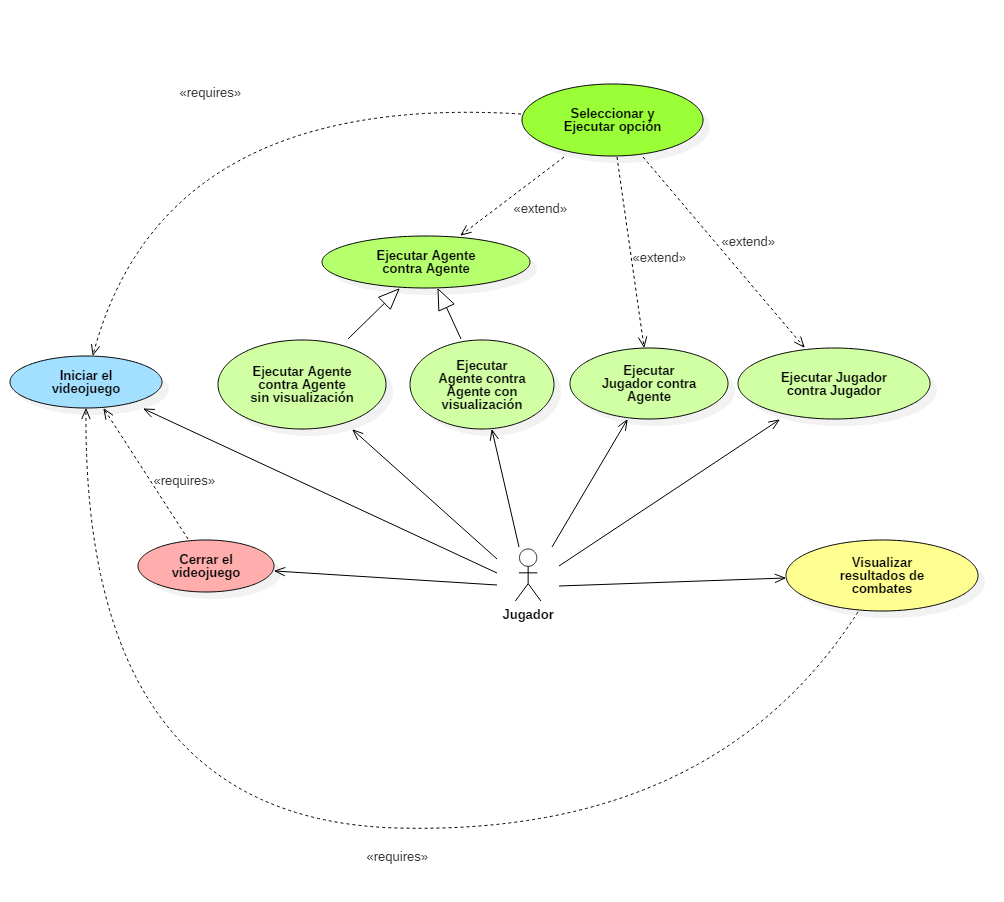
\includegraphics[width=20cm]{diagramas/casosDeUsoCropped.png}}
	\caption{Diagrama de casos de uso}
	\label{casos_de_uso}
\end{figure}

\clearpage

En la figura \ref{casos_de_uso} se muestra el diagrama de casos de uso a partir del cual podremos realizar una definición formal de los mismos. En dicha figura se han agrupado por colores los casos de uso con características similares para facilitar su comprensión y visualización. En este caso se utilizan el color azul y rojo para abrir y cerrar el programa, colores verdes para los diferentes tipos de ejecuciones posibles del combate y el amarillo para ver los resultados de los combates realizados en una ejecución.

\bigskip

A continuación se muestran los casos de uso especificados de manera formal. La notación utilizada para la identificación de los diferentes casos de uso será \textbf{CU\footnote{en referencia a Caso de Uso}-\textit{N\footnote{en referencia al Número asociado al mismo}}}. Los campos presentes en cada descripción contarán con un identificador, nombre, descripción y una prioridad. El nivel de prioridad podrá tener uno de los siguientes tres valores con su significado asociado:

\begin{itemize}
\item \textbf{Vital}: Es fundamental para completar el proyecto.
\item \textbf{Importante}: Aumenta de forma significativa la calidad y funcionamiento del proyecto pero no tiene la cualidad de indispensable.
\item \textbf{Deseable}: Extiende el proyecto pero no debería ser una prioridad.
\end{itemize}

\bigskip



\newcounter{contador_casos_de_uso}
\setcounter{contador_casos_de_uso}{1}

\begin{center}
	\begin{tabular}{ | p{3cm} | p{10cm} | } 
		\hline
		
			\textbf{ID} & CU-\arabic{contador_casos_de_uso}
			\refstepcounter{contador_casos_de_uso} \\
		
		\hline 
		
			\textbf{Nombre} &
			Iniciar el videojuego \\ 
		
		\hline
		
			\textbf{Descripción} & 
			El usuario ejecuta el programa.\\
		
		\hline 
		
			\textbf{Prioridad} &
			Vital\\ 
		
		\hline
	\end{tabular}
\end{center}

\begin{center}
	\begin{tabular}{ | p{3cm} | p{10cm} | } 
		\hline
		
		\textbf{ID} & CU-\arabic{contador_casos_de_uso}
		\refstepcounter{contador_casos_de_uso} \\
		
		\hline 
		
		\textbf{Nombre} &
		Cerrar el videojuego \\ 
		
		\hline
		
		\textbf{Descripción} & 
		El usuario cierra el programa.\\
		
		\hline 
		
		\textbf{Prioridad} &
		Vital\\ 
		
		\hline
	\end{tabular}
\end{center}

\begin{center}
	\begin{tabular}{ | p{3cm} | p{10cm} | } 
		\hline
		
		\textbf{ID} & CU-\arabic{contador_casos_de_uso}
		\refstepcounter{contador_casos_de_uso} \\
		
		\hline 
		
		\textbf{Nombre} &
		Seleccionar y Ejecutar opción \\ 
		
		\hline
		
		\textbf{Descripción} & 
		El usuario escoge una de las opciones posibles para ser ejecutada.\\
		
		\hline 
		
		\textbf{Prioridad} &
		Vital\\ 
		
		\hline
	\end{tabular}
\end{center}


\begin{center}
	\begin{tabular}{ | p{3cm} | p{10cm} | } 
		\hline
		
		\textbf{ID} & CU-\arabic{contador_casos_de_uso}
		\refstepcounter{contador_casos_de_uso} \\
		
		\hline 
		
		\textbf{Nombre} &
		Ejecutar Agente contra Agente \\ 
		
		\hline
		
		\textbf{Descripción} & 
		El usuario escoge una de las opciones en las que el agente compite contra otra versión de sí mismo.\\
		
		\hline 
		
		\textbf{Prioridad} &
		Vital\\ 
		
		\hline
	\end{tabular}
\end{center}


\begin{center}
	\begin{tabular}{ | p{3cm} | p{10cm} | } 
		\hline
		
		\textbf{ID} & CU-\arabic{contador_casos_de_uso}
		\refstepcounter{contador_casos_de_uso} \\
		
		\hline 
		
		\textbf{Nombre} &
		Ejecutar Agente contra Agente con visualización \\ 
		
		\hline
		
		\textbf{Descripción} & 
		El usuario escoge la opción de visualizar un combate entre un agente y otra versión de sí mismo.\\
		
		\hline 
		
		\textbf{Prioridad} &
		Vital\\ 
		
		\hline
	\end{tabular}
\end{center}

\begin{center}
	\begin{tabular}{ | p{3cm} | p{10cm} | } 
		\hline
		
		\textbf{ID} & CU-\arabic{contador_casos_de_uso}
		\refstepcounter{contador_casos_de_uso} \\
		
		\hline 
		
		\textbf{Nombre} &
		Ejecutar Agente contra Agente sin visualización \\ 
		
		\hline
		
		\textbf{Descripción} & 
		El usuario escoge la opción de simular un combate entre un agente y otra versión de sí mismo sin realizar una visualización del mismo.\\
		
		\hline 
		
		\textbf{Prioridad} &
		Vital\\ 
		
		\hline
	\end{tabular}
\end{center}

\begin{center}
	\begin{tabular}{ | p{3cm} | p{10cm} | } 
		\hline
		
		\textbf{ID} & CU-\arabic{contador_casos_de_uso}
		\refstepcounter{contador_casos_de_uso} \\
		
		\hline 
		
		\textbf{Nombre} &
		Ejecutar Jugador contra Agente\\ 
		
		\hline
		
		\textbf{Descripción} & 
		El usuario escoge la opción que le permite competir contra el agente.\\
		
		\hline 
		
		\textbf{Prioridad} &
		Vital\\ 
		
		\hline
	\end{tabular}
\end{center}


\begin{center}
	\begin{tabular}{ | p{3cm} | p{10cm} | } 
		\hline
		
		\textbf{ID} & CU-\arabic{contador_casos_de_uso}
		\refstepcounter{contador_casos_de_uso} \\
		
		\hline 
		
		\textbf{Nombre} &
		Ejecutar Jugador contra Jugador\\ 
		
		\hline
		
		\textbf{Descripción} & 
		El usuario escoge la opción que le permite competir contra otro usuario.\\
		
		\hline 
		
		\textbf{Prioridad} &
		Importante\\ 
		
		\hline
	\end{tabular}
\end{center}

\begin{center}
	\begin{tabular}{ | p{3cm} | p{10cm} | } 
		\hline
		
		\textbf{ID} & CU-\arabic{contador_casos_de_uso}
		\refstepcounter{contador_casos_de_uso} \\
		
		\hline 
		
		\textbf{Nombre} &
		Visualizar resultados de combates\\ 
		
		\hline
		
		\textbf{Descripción} & 
		El usuario visualiza los resultados acumulados de los combates que han ocurrido en la ejecución del programa.\\
		
		\hline 
		
		\textbf{Prioridad} &
		Deseable\\
		
		\hline
	\end{tabular}
\end{center}


\subsection{Especificación de requisitos}

Una vez definidos los casos de uso se puede proceder a realizar un análisis detenido de cada uno de ellos para así extraer los requisitos que se deben cumplir para hacer posible su ejecución. Esta sección estará dedicada a clasificar y describir con el menor grado de ambigüedad posibles cada uno de los requisitos del proyecto. Para este fin utilizaremos el estándar IEEE830 \cite{ieee}, en el que se define la diferenciación entre tres tipos de requisitos:

\begin{itemize}
\item \textbf{Requisitos de información}: Identificados con códigos de la forma RI-\textit{N}
\item \textbf{Requisitos funcionales}: Identificados con códigos de la forma RF-\textit{N}
\item \textbf{Requisitos no funcionales}: Identificados con códigos de la forma RNF-\textit{N}
\end{itemize}

Algunos de los campos que se utilizarán para describir los requisitos son comunes, tales como el identificador (ID), nombre, descripción y criticidad. En aras de mantener un buen nivel de consistencia se utilizará una escala similar a la de la importancia de los casos de uso para definir la criticidad, pudiendo tomar la misma los siguientes valores:

\begin{itemize}
	\item \textbf{Vital}: Es fundamental para completar el proyecto.
	\item \textbf{Importante}: Aumenta de forma significativa la calidad y funcionamiento del proyecto pero no tiene la cualidad de indispensable.
	\item \textbf{Deseable}: Extiende el proyecto pero no debería ser una prioridad.
\end{itemize}

\bigskip

\subsubsection{Requisitos de información}

Este subapartado contendrá los requisitos de información del proyecto. Este tipo de requisito especifica los datos que deberán ser almacenados por el sistema para permitir así el cumplimiento de otros requisitos ya sea de forma parcial o total. A continuación se muestran formalmente los requisitos de información del proyecto:

\newcounter{contador_requisitos_de_informacion}
\setcounter{contador_requisitos_de_informacion}{1}


\begin{center}
	\begin{tabular}{ | p{4.5cm} | p{10cm} | } 
		\hline
		
		\textbf{ID} & RI-\arabic{contador_requisitos_de_informacion}
		\refstepcounter{contador_requisitos_de_informacion} \\
		
		\hline 
		
		\textbf{Nombre} &
		Datos aprendidos por el agente\\ 
		
		\hline
		
		\textbf{Requisitos asociados} & 
		\begin{itemize}
			\item RF-5: Salir de la aplicación
			\item RF-7: Moverse en el área de combate
			\item RF-8: Atacar al enemigo
			\item RF-9: Defenderse del enemigo
			\item RF-13: Visualizar combate entre agentes
			\item RF-14: Simular múltiples combates
		\end{itemize}\\
		
		\hline
		
		\textbf{Descripción} & 
		El sistema deberá almacenar los datos que representan el conocimiento aprendido por el agente, sea cual sea su forma.\\
		
		\hline 
		
		\textbf{Datos específicos} &
		\begin{itemize}
			\item Estados visitados previamente por el agente
			\item Acciones tomadas por el agente en un determinado estado
			\item Resultado, positivo o negativo, de las acciones tomadas en un estado determinado.
		\end{itemize}\\
		
		\hline 
		
		\textbf{Criticidad} &
		Vital\\
		
		\hline
	\end{tabular}
\end{center}

\begin{center}
	\begin{tabular}{ | p{4.5cm} | p{10cm} | } 
		\hline
		
		\textbf{ID} & RI-\arabic{contador_requisitos_de_informacion}
		\refstepcounter{contador_requisitos_de_informacion} \\
		
		\hline 
		
		\textbf{Nombre} &
		Archivos necesarios para la ejecución del videojuego\\ 
		
		\hline
		
		\textbf{Requisitos asociados} & 
		Todos los requisitos funcionales están asociados ya que para todas las funcionalidades es necesario tener acceso a estos archivos.\\
		
		\hline
		
		\textbf{Descripción} & 
		El sistema deberá almacenar todos los archivos no relacionados con el código de la aplicación en si misma que se requieren para mostrar los contenidos de la aplicación\\
		
		\hline 
		
		\textbf{Datos específicos} &
		\begin{itemize}
			\item Imágenes que contienen las animaciones de los personajes.
			\item Archivos de audio que contienen los diferentes sonidos del videojuego.
			\item Archivos que contienen las diferentes fuentes usadas para mostrar el texto por pantalla.
			\item Archivos que contienen los "Shaders"\footnote{Programas que se ejecutan en la targeta gráfica a la hora de mostrar cada pixel en la pantalla} utilizados para los diferentes efectos dentro del videojuego.
		\end{itemize}\\
		
		\hline 
		
		\textbf{Criticidad} &
		Vital\\
		
		\hline
	\end{tabular}
\end{center}



\subsubsection{Requisitos funcionales}

Los requisitos funcionales son utilizados para definir las funciones que un sistema debe ser capaz de realizar, definiendo de esta forma el comportamiento que tendrá el software a nivel interno. La especificación de los mismos muestra como, a partir de su cumplimiento, se llevarán a la práctica los casos de uso definidos para el proyecto.


\newcounter{contador_requisitos_funcionales}
\setcounter{contador_requisitos_funcionales}{1}

\begin{center}
	\begin{tabular}{ | p{4.7cm} | p{10cm} | } 
		\hline
		
		\textbf{ID} & RF-\arabic{contador_requisitos_funcionales}
		\refstepcounter{contador_requisitos_funcionales} \\
		
		\hline 
		\textbf{Nombre}&
		Visualizar el menú\\ 
		
		\hline
		\textbf{Requisitos asociados} & 
		\begin{itemize}
			\item RF-2: Moverse en el menú
			\item RF-3: Ejecutar una opción del menú
			\item RF-12: Volver al menú
		\end{itemize}\\
		
		\hline
		\textbf{Descripción} & 
		El sistema deberá mostrar un menú con las diferentes opciones de combate que es posible ejecutar en la aplicación.\\
		
		\hline
		\textbf{Precondición} & 
		Ninguna
		\\
		
		\hline
		\textbf{Secuencia normal} &
		\begin{enumerate}
			\item El usuario ejecuta la aplicación.
			\item El usuario visualiza las opciones disponibles distinguiendo la preseleccionada por defecto.
		\end{enumerate}
		\\
		
		\hline
		\textbf{Secuencia alternativa 1} &
		\begin{enumerate}
			\item El vuelve al menú después de un combate.
			\item El usuario visualiza las opciones disponibles distinguiendo la preseleccionada por defecto.
		\end{enumerate}
		\\
		
		\hline
		\textbf{Postcondición} & 
		Se pueden ver y distinguir todas las opciones del menú y seleccionar una de ellas.
		\\
		
		\hline 
		\textbf{Criticidad} &
		Vital\\
		
		\hline 
		\textbf{Criterio de validación} & 
		Se considerará este requisito como aceptado cuando el usuario pueda visualizar correctamente el menú sea cual sea la forma en la que se llegue a él (primera ejecución o después de combate).\\
		
		\hline
	\end{tabular}
\end{center}

\begin{center}
	\begin{tabular}{ | p{4.7cm} | p{10cm} | } 
		\hline
		
		\textbf{ID} & RF-\arabic{contador_requisitos_funcionales}
		\refstepcounter{contador_requisitos_funcionales} \\
		
		\hline 
		\textbf{Nombre} &
		Moverse en el menú\\ 
		
		\hline
		\textbf{Requisitos asociados} & 
		\begin{itemize}
			\item RF-1: Visualizar el menú
			\item RF-3: Ejecutar una opción del menú
			\item RF-12: Volver al menú
		\end{itemize}\\
		
		\hline
		\textbf{Descripción} & 
		El sistema debe permitir viajar entre las diferentes opciones del menú mostrando claramente que opción es la seleccionada actualmente.\\
		
		\hline
		\textbf{Precondición} & 
		Se esta visualizando el menú de la aplicación.\\
		
		\hline
		\textbf{Secuencia normal} &
		 \begin{enumerate}
		 	\item El usuario pulsa el botón para moverse en el menú (hacia arriba o abajo).
		 \end{enumerate}
		\\
		
		\hline
		\textbf{Postcondición} & 
		Se cambia la opción seleccionada a la siguiente o anterior dependiendo del botón pulsado, abajo o arriba respectivamente.
		\\
		
		\hline 
		\textbf{Criticidad} &
		Vital\\
		
		\hline 
		\textbf{Criterio de validación} & 
		Se considerará este requisito como aceptado cuando el usuario pueda cambiar de opción en el menú utilizando los botones dedicados a ello y se visualice dicho cambio de forma inequívoca.\\
		
		\hline
	\end{tabular}
\end{center}


\begin{center}
	\begin{tabular}{ | p{4.7cm} | p{10cm} | } 
		\hline
		
		\textbf{ID} & RF-\arabic{contador_requisitos_funcionales}
		\refstepcounter{contador_requisitos_funcionales} \\
		
		\hline 
		\textbf{Nombre} &
		Ejecutar una opción del menú\\ 
		
		\hline
		\textbf{Requisitos asociados} & 
		\begin{itemize}
			\item RF-1: Visualizar el menú
			\item RF-2: Moverse en el menú
			\item RF-12: Volver al menú
		\end{itemize}\\
		
		\hline
		\textbf{Descripción} & 
		El sistema deberá permitir la ejecución de la opción actualmente seleccionada en el menú de la aplicación.\\
		
		\hline
		\textbf{Precondición} & 
		Se está visualizando el menú de la aplicación y hay una opción seleccionada.\\
		
		\hline
		\textbf{Secuencia normal} &
		\begin{enumerate}
			\item El usuario pulsa el botón de ejecutar la opción seleccionada del menú.
		\end{enumerate}
		\\
		
		\hline
		\textbf{Postcondición} & 
		Se ejecuta la acción seleccionada y se pasa a la escena asociada a dicha acción.\\
		
		\hline 
		\textbf{Criticidad} &
		Vital\\
		
		\hline 
		\textbf{Criterio de validación} & 
		Se considerará este requisito como aceptado cuando el usuario pueda ejecutar todas las opciones del menú y se pase a la escena que se ha asociado con cada una de ellas.\\
		
		\hline
	\end{tabular}
\end{center}

\begin{center}
	\begin{tabular}{ | p{4.7cm} | p{10cm} | } 
		\hline
		
		\textbf{ID} & RF-\arabic{contador_requisitos_funcionales}
		\refstepcounter{contador_requisitos_funcionales} \\
		
		\hline 
		\textbf{Nombre} &
		Alternar apertura de la consola con resultados\\ 
		
		\hline
		\textbf{Requisitos asociados} & 
		\begin{itemize}
			\item RF-4: Alternar apertura de la consola con resultados
		\end{itemize}\\
		
		\hline
		\textbf{Descripción} & 
		El sistema deberá permitir alternar entre la apertura y cierre de una consola donde se muestren los resultados de los combates previos realizados en esa ejecución del programa.\\
		
		\hline
		\textbf{Precondición} & 
		Se han ejecutado combates en la presente ejecución del programa.\\
		
		\hline
		\textbf{Secuencia normal} &
		\begin{enumerate}
			\item El usuario pulsa el botón de abrir/cerrar la consola.
		\end{enumerate}
		\\
		
		\hline
		\textbf{Postcondición} & 
		La consola cambia al estado de visualización distinto al que estaba, se cierra si estaba abierta y se abre si estaba cerrada.\\
		
		\hline 
		\textbf{Criticidad} &
		Importante\\
		
		\hline 
		\textbf{Criterio de validación} & 
		Se considerará este requisito como aceptado si la apertura y cierre de la consola de resultados es funcional en cualquier estado posible en el que el usuario pueda visualizar la aplicación.\\
		
		\hline
	\end{tabular}
\end{center}

\begin{center}
	\begin{tabular}{ | p{4.7cm} | p{10cm} | } 
		\hline
		
		\textbf{ID} & RF-\arabic{contador_requisitos_funcionales}
		\refstepcounter{contador_requisitos_funcionales} \\
		
		\hline 
		\textbf{Nombre} &
		Salir de la aplicación\\ 
		
		\hline
		\textbf{Descripción} & 
		El sistema deberá permitir salir de la aplicación sea cual sea el estado en el que se encuentre y sin producir errores ni en la presente ni en futuras ejecuciones.\\
		
		\hline
		\textbf{Precondición} & 
		La aplicación está en ejecución en cualquier estado.\\
		
		\hline
		\textbf{Secuencia normal} &
		\begin{enumerate}
			\item El usuario ejecuta la opción del menú dedicada a cerrar la aplicación.
		\end{enumerate}
		\\
		
		\hline
		\textbf{Secuencia alternativa 1} &
		\begin{enumerate}
			\item El usuario cierra la ventana de la aplicación haciendo uso de las funcionalidades del sistema de ventanas.
		\end{enumerate}
		\\
		
		\hline
		\textbf{Postcondición} & 
		Se ha terminado la ejecución de la aplicación.\\
		
		\hline 
		\textbf{Criticidad} &
		Vital\\
		
		\hline 
		\textbf{Criterio de validación} & 
		Se considerará este requisito como aceptado si el cierre de la aplicación no produce errores sea cual sea el estado actual del programa y usando una de las dos secuencias explicadas.\\
		
		\hline
	\end{tabular}
\end{center}

\begin{center}
	\begin{tabular}{ | p{4.7cm} | p{10cm} | } 
		\hline
		
		\textbf{ID} & RF-\arabic{contador_requisitos_funcionales}
		\refstepcounter{contador_requisitos_funcionales} \\
		
		\hline 
		\textbf{Nombre} &
		Entrar en la escena del combate\\ 
		
		\hline
		\textbf{Requisitos asociados} & 
		\begin{itemize}
			\item RF-3: Ejecutar una opción del menú
		\end{itemize}\\
		
		\hline
		\textbf{Descripción} & 
		El sistema deberá permitir cambiar a una escena de combate si así lo requiere la ejecución de una de las opciones del menú. Al realizar esta acción se visualizará el combate y se podrá interactuar con el enemigo.\\
		
		\hline
		\textbf{Precondición} & 
		Se ha seleccionado una de las opciones del menú que requiere pasar a la escena del combate.\\
		
		\hline
		\textbf{Secuencia normal} &
		\begin{enumerate}
			\item El usuario pulsa el botón de entrar en la escena del combate. 
		\end{enumerate}
		\\
		
		\hline
		\textbf{Postcondición} & 
		La aplicación se encuentra ahora en una escena de combate.\\
		
		\hline 
		\textbf{Criticidad} &
		Vital\\
		
		\hline 
		\textbf{Criterio de validación} & 
		Se considerará este requisito como aceptado si se entra en una escena de combate al pulsar una opción del menú que lo requiera.\\
		
		\hline
	\end{tabular}
\end{center}

\begin{center}
	\begin{tabular}{ | p{4.7cm} | p{10cm} | } 
		\hline
		
		\textbf{ID} & RF-\arabic{contador_requisitos_funcionales}
		\refstepcounter{contador_requisitos_funcionales} \\
		
		\hline 
		\textbf{Nombre} &
		Moverse en el área de combate.\\ 
		
		\hline
		\textbf{Requisitos asociados} & 
		\begin{itemize}
			\item RF-8: Atacar al enemigo
			\item RF-9: Defenderse del enemigo
		\end{itemize}\\
		
		\hline
		\textbf{Descripción} & 
		El sistema deberá permitir que el usuario mueva a su personaje en el contexto del combate.\\
		
		\hline
		\textbf{Precondición} & 
		La aplicación se encuentra en una escena de combate.\\
		
		\hline
		\textbf{Secuencia normal} &
		\begin{enumerate}
			\item El usuario mueve la palanca o \textit{"joystick"} en la dirección que quiere mover su personaje.
		\end{enumerate}
		\\
		
		\hline
		\textbf{Postcondición} & 
		El personaje se mueve en la dirección indicada por el usuario.\\
		
		\hline 
		\textbf{Criticidad} &
		Vital\\
		
		\hline 
		\textbf{Criterio de validación} & 
		Se considerará este requisito como aceptado si el personaje se mueve hacia la dirección indicada por el usuario.\\
		
		\hline
	\end{tabular}
\end{center}

\begin{center}
	\begin{tabular}{ | p{4.7cm} | p{10cm} | } 
		\hline
		
		\textbf{ID} & RF-\arabic{contador_requisitos_funcionales}
		\refstepcounter{contador_requisitos_funcionales} \\
		
		\hline 
		\textbf{Nombre} &
		Atacar al enemigo\\ 
		
		\hline
		\textbf{Requisitos asociados} & 
		\begin{itemize}
			\item RF-7: Moverse en el área de combate
			\item RF-9: Defenderse del enemigo
		\end{itemize}\\
		
		\hline
		\textbf{Descripción} & 
		El sistema deberá permitir que un personaje dañe a otro mediante la utilización de un ataque.\\
		
		\hline
		\textbf{Precondición} & 
		La aplicación se encuentra en una escena de combate.\\
		
		\hline
		\textbf{Secuencia normal} &
		\begin{enumerate}
			\item El usuario pulsa el botón de atacar.
		\end{enumerate}
		\\
		
		\hline
		\textbf{Secuencia alternativa 1} &
		\begin{enumerate}
			\item El agente decide realizar la acción de atacar.
		\end{enumerate}
		\\
		
		\hline
		\textbf{Postcondición} & 
		El personaje que debe realizar la acción de atacar comienza la ejecución del ataque.\\
		
		\hline 
		\textbf{Criticidad} &
		Vital\\
		
		\hline 
		\textbf{Criterio de validación} & 
		Se considerará este requisito como aceptado si tanto el usuario como el agente son capaces de atacar cuando deciden realizar esa acción dentro de la escena de combate.\\
		
		\hline
	\end{tabular}
\end{center}

\begin{center}
	\begin{tabular}{ | p{4.7cm} | p{10cm} | } 
		\hline
		
		\textbf{ID} & RF-\arabic{contador_requisitos_funcionales}
		\refstepcounter{contador_requisitos_funcionales} \\
		
		\hline 
		\textbf{Nombre} &
		Defenderse del enemigo\\ 
		
		\hline
		\textbf{Requisitos asociados} & 
		\begin{itemize}
			\item RF-7: Moverse en el área de combate
			\item RF-8: Atacar al enemigo
		\end{itemize}\\
		
		\hline
		\textbf{Descripción} & 
		El sistema deberá permitir que un usuario realice una acción defensiva contra su contrincante de forma que no pueda recibir daño.\\
		
		\hline
		\textbf{Precondición} & 
		La aplicación se encuentra en una escena de combate.\\
		
		\hline
		\textbf{Secuencia normal} &
		\begin{enumerate}
			\item El usuario pulsa el botón de defenderse.
		\end{enumerate}
		\\
		
		\hline
		\textbf{Secuencia alternativa 1} &
		\begin{enumerate}
			\item El agente decide realizar la acción de defenderse.
		\end{enumerate}
		\\
		
		\hline
		\textbf{Postcondición} & 
		El personaje que debe realizar la acción de defenderse se encuentra en un estado en el que no puede recibir daño.\\
		
		\hline 
		\textbf{Criticidad} &
		Vital\\
		
		\hline 
		\textbf{Criterio de validación} & 
		Se considerará este requisito como aceptado si el personaje se encuentra en un estado de defensa cuando deciden realizar esta acción dentro de la escena de combate.\\
		
		\hline
	\end{tabular}
\end{center}

\begin{center}
	\begin{tabular}{ | p{4.7cm} | p{10cm} | } 
		\hline
		
		\textbf{ID} & RF-\arabic{contador_requisitos_funcionales}
		\refstepcounter{contador_requisitos_funcionales} \\
		
		\hline 
		\textbf{Nombre} &
		Ganar/Perder partida\\ 
		
		\hline
		\textbf{Requisitos asociados} & 
		\begin{itemize}
			\item RF-11: Agotar el tiempo de combate
		\end{itemize}\\
		
		\hline
		\textbf{Descripción} & 
		El sistema deberá permitir que uno de los personajes gane la partida si la vida de su contrincante llega a cero. Haciendo de forma efectiva que uno de los personajes pierda y otro gane.\\
		
		\hline
		\textbf{Precondición} & 
		La aplicación se encuentra una escena de combate.\\
		
		\hline
		\textbf{Secuencia normal} &
		\begin{enumerate}
			\item Uno de los personajes lleva a cabo una acción que desemboca en que la vida de uno de ellos llegue a cero.
		\end{enumerate}
		\\
		
		\hline
		\textbf{Postcondición} & 
		Se muestra por pantalla claramente cual de los personajes ha ganado y se detiene el combate.\\
		
		\hline 
		\textbf{Criticidad} &
		Vital\\
		
		\hline 
		\textbf{Criterio de validación} & 
		Se considerará este requisito como aceptado si siempre que la vida de uno de los personajes llegue a cero se detiene la pelea y se nombre ganador de la misma al personaje superviviente.\\
		
		\hline
	\end{tabular}
\end{center}

\begin{center}
	\begin{tabular}{ | p{4.7cm} | p{10cm} | } 
		\hline
		
		\textbf{ID} & RF-\arabic{contador_requisitos_funcionales}
		\refstepcounter{contador_requisitos_funcionales} \\
		
		\hline 
		\textbf{Nombre} &
		Agotar el tiempo de combate\\ 
		
		\hline
		\textbf{Requisitos asociados} & 
		\begin{itemize}
			\item RF-10: Ganar/Perder partida
		\end{itemize}\\
		
		\hline
		\textbf{Descripción} & 
		La aplicación deberá permitir que un combate termine sin que la vida de uno de los personajes llegue a cero si se termina el tiempo máximo establecido.\\
		
		\hline
		\textbf{Precondición} & 
		La aplicación se encuentra en una escena de combate.\\
		
		\hline
		\textbf{Secuencia normal} &
		\begin{enumerate}
			\item El usuario espera a que el tiempo de combate llegue a cero.
		\end{enumerate}
		\\
		
		\hline
		\textbf{Postcondición} & 
		Se detiene el combate.\\
		
		\hline 
		\textbf{Criticidad} &
		Importante\\
		
		\hline 
		\textbf{Criterio de validación} & 
		Se considerará este requisito como aceptado si sea cual sea el estado de un combate este se detiene al llegar el tiempo disponible para el mismo a cero.\\
		
		\hline
	\end{tabular}
\end{center}

\begin{center}
	\begin{tabular}{ | p{4.7cm} | p{10cm} | } 
		\hline
		
		\textbf{ID} & RF-\arabic{contador_requisitos_funcionales}
		\refstepcounter{contador_requisitos_funcionales} \\
		
		\hline 
		\textbf{Nombre} &
		Volver al menú\\ 
		
		\hline
		\textbf{Requisitos asociados} & 
		\begin{itemize}
			\item RF-1: Visualizar el menú
		\end{itemize}\\
		
		\hline
		\textbf{Descripción} & 
		El sistema deberá permitir volver al menú principal desde la escena de combate.\\
		
		\hline
		\textbf{Precondición} & 
		La aplicación se encuentra en una escena de combate.\\
		
		\hline
		\textbf{Secuencia normal} &
		\begin{enumerate}
			\item El usuario pulsa el botón de volver al menú.
		\end{enumerate}
		\\
		
		\hline
		\textbf{Postcondición} & 
		Se detiene la pelea y se vuelve al menú de la aplicación.\\
		
		\hline 
		\textbf{Criticidad} &
		Importante\\
		
		\hline 
		\textbf{Criterio de validación} & 
		Se considerará este requisito como aceptado si siempre que la aplicación se encuentre mostrando una escena de combate es posible volver al menú principal utilizando el botón dedicado para ello.\\
		
		\hline
	\end{tabular}
\end{center}

\begin{center}
	\begin{tabular}{ | p{4.7cm} | p{10cm} | } 
		\hline
		
		\textbf{ID} & RF-\arabic{contador_requisitos_funcionales}
		\refstepcounter{contador_requisitos_funcionales} \\
		
		\hline 
		\textbf{Nombre} &
		Visualizar combate entre agentes\\ 
		
		\hline
		\textbf{Requisitos asociados} & 
		\begin{itemize}
			\item RF-6: Entrar en la escena de combate
			\item RF-10: Ganar/Perder partida
			\item RF-11: Agotar el tiempo de combate
		\end{itemize}\\
		
		\hline
		\textbf{Descripción} & 
		El sistema deberá permitir visualizar la totalidad de un combate entre el agente y otra versión de si mismo sin que el usuario tenga que controlar a ningún personaje dentro de la escena de combate.\\
		
		\hline
		\textbf{Precondición} & 
		Se ejecuta la opción del menú dedicada a visualizar el combate entre dos agentes.\\
		
		\hline
		\textbf{Secuencia normal} &
		\begin{enumerate}
			\item El usuario pulsa el botón dedicado a comenzar la pelea entre dos agentes.
		\end{enumerate}
		\\
		
		\hline
		\textbf{Postcondición} & 
		Se entra en la escena de combate con los dos personajes siendo controlados por un agente.\\
		
		\hline 
		\textbf{Criticidad} &
		Vital\\
		
		\hline 
		\textbf{Criterio de validación} & 
		Se considerará este requisito como aceptado si se puede visualizar un combate completo entre un agente y otra versión de si mismo de la misma forma que se visualizaría un combate entre regular entre el usuario y un agente o entre dos usuarios.\\
		
		\hline
	\end{tabular}
\end{center}

\begin{center}
	\begin{tabular}{ | p{4.7cm} | p{10cm} | } 
		\hline
		
		\textbf{ID} & RF-\arabic{contador_requisitos_funcionales}
		\refstepcounter{contador_requisitos_funcionales} \\
		
		\hline 
		\textbf{Nombre} &
		Simular múltiples combates\\ 
		
		\hline
		\textbf{Requisitos asociados} & 
		\begin{itemize}
			\item RF-6: Entrar en la escena de combate
		\end{itemize}\\
		
		\hline
		\textbf{Descripción} & 
		El sistema deberá permitir que se realicen varios combates entre dos versiones del agente de forma acelerada para permitir que el mismo complete el proceso de aprendizaje en un tiempo razonable.\\
		
		\hline
		\textbf{Precondición} & 
		Se ejecuta la opción del menú dedicada a simular varios combates entre dos agentes.\\
		
		\hline
		\textbf{Secuencia normal} &
		\begin{enumerate}
			\item El usuario pulsa el botón dedicado a simular varios combates entre agentes.
		\end{enumerate}
		\\
		
		\hline
		\textbf{Postcondición} & 
		Se comienza la simulación de los combates.\\
		
		\hline 
		\textbf{Criticidad} &
		Vital\\
		
		\hline 
		\textbf{Criterio de validación} & 
		Se considerará este requisito como aceptado si se pueden realizar varias simulaciones de forma iterativa en las que el agente visite los diferentes estados.\\
		
		\hline
	\end{tabular}
\end{center}

\begin{center}
	\begin{tabular}{ | p{4.7cm} | p{10cm} | } 
		\hline
		
		\textbf{ID} & RF-\arabic{contador_requisitos_funcionales}
		\refstepcounter{contador_requisitos_funcionales} \\
		
		\hline 
		\textbf{Nombre} &
		Comandos en la consola\\ 
		
		\hline
		\textbf{Requisitos asociados} & 
		\begin{itemize}
			\item RF-4: Alternar apertura de la consola con resultados
		\end{itemize}\\
		
		\hline
		\textbf{Descripción} & 
		El sistema deberá permitir ejecutar comandos utilizando la consola para realizar acciones específicas dentro de la aplicación de forma aislada.\\
		
		\hline
		\textbf{Precondición} & 
		La consola de la aplicación está siendo visualizada.\\
		
		\hline
		\textbf{Secuencia normal} &
		\begin{enumerate}
			\item El usuario introduce un comando en formato de texto en la consola.
			\item El usuario pulsa el botón de ejecutar el comando.
			\item El usuario visualiza el resultado.
		\end{enumerate}
		\\
		
		\hline
		\textbf{Excepciones secuencia normal} &
		\begin{enumerate}
			\setcounter{enumi}{3}
			\item El usuario no percibe ningún resultado porque el comando no existe.
		\end{enumerate}
		\\
		
		\hline
		\textbf{Postcondición} & 
		El comando ha sido procesado y ejecutado.\\
		
		\hline 
		\textbf{Criticidad} &
		Deseable\\
		
		\hline 
		\textbf{Criterio de validación} & 
		Se considerará este requisito como aceptado si se puede ejecutar un comando en la consola de la aplicación de forma que si el mismo es correcto se ejecute y si no lo es no ocurra nada.\\
		
		\hline
	\end{tabular}
\end{center}

\clearpage

\subsubsection{Requisitos no funcionales}

\newcounter{contador_requisitos_no_funcionales}
\setcounter{contador_requisitos_no_funcionales}{1}

Los requisitos no funcionales especifican necesidades del sistema referentes a su operación, esto puede referirse a rendimiento, tiempos de respuesta, capacidad, etc. Al contrario que los requisitos funcionales, los requisitos no funcionales se centran en las características de funcionamiento de esas funcionalidades y no en las funcionalidades en si mismas.

\bigskip 

En este apartado se definirán los requisitos no funcionales de este proyecto formalmente:

\begin{center}
	\begin{tabular}{ | p{4.7cm} | p{10cm} | } 
		\hline
		
		\textbf{ID} & RNF-\arabic{contador_requisitos_no_funcionales}
		\refstepcounter{contador_requisitos_no_funcionales} \\
		
		\hline 
		\textbf{Nombre} &
		Rendimiento de la aplicación\\ 
		
		\hline
		\textbf{Descripción} & 
		La aplicación, especialmente en las escenas de combate, deberá visualizarse a 60 fotogramas por segundo para garantizar la fluidez de cara al usuario.\\
		
		\hline 
		\textbf{Criticidad} &
		Importante\\
		
		\hline 
		\textbf{Criterio de validación} & 
		Se considerará este requisito como cumplido si durante un número suficiente de combates consecutivos, los fotogramas por segundo medios de la aplicación no caen por debajo de 60.\\
		
		\hline
	\end{tabular}
\end{center}


\begin{center}
	\begin{tabular}{ | p{4.7cm} | p{10cm} | } 
		\hline
		
		\textbf{ID} & RNF-\arabic{contador_requisitos_no_funcionales}
		\refstepcounter{contador_requisitos_no_funcionales} \\
		
		\hline 
		\textbf{Nombre} &
		Velocidad de las simulaciones\\ 
		
		\hline
		\textbf{Descripción} & 
		En aras de permitir la realización del proceso de aprendizaje del agente en un tiempo razonable se deberá permitir la simulación de combates con el tiempo interno del juego sustancialmente acelerado.\\
		
		\hline 
		\textbf{Criticidad} &
		Vital\\
		
		\hline 
		\textbf{Criterio de validación} & 
		Se considerará este requisito como cumplido si el agente es capaz de competir con una de las implementaciones basadas en reglas y ganar más de un 50\% de las veces después de menos de 15 minutos de entrenamiento.\\
		
		\hline
	\end{tabular}
\end{center}

\begin{center}
	\begin{tabular}{ | p{4.7cm} | p{10cm} | } 
		\hline
		
		\textbf{ID} & RNF-\arabic{contador_requisitos_no_funcionales}
		\refstepcounter{contador_requisitos_no_funcionales} \\
		
		\hline 
		\textbf{Nombre} &
		Extensibilidad del motor\\ 
		
		\hline
		\textbf{Descripción} & 
		La aplicación deberá de estar correctamente separada en subsistemas independientes conectados mediante un bus de mensajes que permita agregar nuevos subsistemas sin afectar a los existentes.\\
		
		\hline 
		\textbf{Criticidad} &
		Importante\\
		
		\hline 
		\textbf{Criterio de validación} & 
		Se considerará este requisito como cumplido si se sigue el patrón de arquitectura de bus de mensajes y se puede agregar un nuevo subsistema sin hacer ninguna modificación a los existentes.\\
		
		\hline
	\end{tabular}
\end{center}

\begin{center}
	\begin{tabular}{ | p{4.7cm} | p{10cm} | } 
		\hline
		
		\textbf{ID} & RNF-\arabic{contador_requisitos_no_funcionales}
		\refstepcounter{contador_requisitos_no_funcionales} \\
		
		\hline 
		\textbf{Nombre} &
		Facilidad para depurar\\ 
		
		\hline
		\textbf{Descripción} & 
		Se debe permitir ejecutar la ejecución de comandos en tiempo de ejecución para facilitar la depuración de subsistemas concretos.\\
		
		\hline 
		\textbf{Criticidad} &
		Deseable\\
		
		\hline 
		\textbf{Criterio de validación} & 
		Se considerará este requisito como cumplido si se pueden insertar mensajes en el bus de mensajes que conecta los subsistemas que componen el programa desde la consola de la aplicación.\\
		
		\hline
	\end{tabular}
\end{center}

\begin{center}
	\begin{tabular}{ | p{4.7cm} | p{10cm} | } 
		\hline
		
		\textbf{ID} & RNF-\arabic{contador_requisitos_no_funcionales}
		\refstepcounter{contador_requisitos_no_funcionales} \\
		
		\hline 
		\textbf{Nombre} &
		Aplicación autocontenida\\ 
		
		\hline
		\textbf{Descripción} & 
		La aplicación deberá de poder ser distribuida de forma que no se requiera la instalación de frameworks, librerías externas u otro archivos para su ejecución.\\
		
		\hline 
		\textbf{Criticidad} &
		Importante\\
		
		\hline 
		\textbf{Criterio de validación} & 
		Se considerará este requisito como cumplido si se puede ejecutar la aplicación sin realizar ningún cambio sobre una instalación limpia de los sistemas operativos para los que se ha construido. Además todos los archivos que requiera la aplicación deberán estar dentro del ejecutable, siendo su existencia transparente al usuario.\\
		
		\hline
	\end{tabular}
\end{center}


\begin{center}
	\begin{tabular}{ | p{4.7cm} | p{10cm} | } 
		\hline
		
		\textbf{ID} & RNF-\arabic{contador_requisitos_no_funcionales}
		\refstepcounter{contador_requisitos_no_funcionales} \\
		
		\hline 
		\textbf{Nombre} &
		Extensibilidad en términos de escenas\\ 
		
		\hline
		\textbf{Descripción} & 
		La aplicación se deberá de componer por escenas de forma que siempre haya solamente una escena activa, pudiendo cambiar entre diferentes escenas con facilidad y agregar nuevas escenas si es necesario.\\
		
		\hline 
		\textbf{Criticidad} &
		Importante\\
		
		\hline 
		\textbf{Criterio de validación} & 
		Se considerará este requisito como cumplido si se pueden agregar escenas a la aplicación y cambiar entre ellas sin hacer ninguna modificación sobre el código que existía previamente tanto en términos de escenas como del propio motor.\\
		
		\hline
	\end{tabular}
\end{center}

\begin{center}
	\begin{tabular}{ | p{4.7cm} | p{10cm} | } 
		\hline
		
		\textbf{ID} & RNF-\arabic{contador_requisitos_no_funcionales}
		\refstepcounter{contador_requisitos_no_funcionales} \\
		
		\hline 
		\textbf{Nombre} &
		Documentación\\ 
		
		\hline
		\textbf{Descripción} & 
		La documentación generada para el proyecto debe priorizar la claridad y simplicidad cuando sea posible. Teniendo en cuenta los conocimientos de los lectores para los que está orientada.\\
		
		\hline 
		\textbf{Criticidad} &
		Importante\\
		
		\hline 
		\textbf{Criterio de validación} & 
		Se considerará este requisito como cumplido si la documentación carece de apartados o secciones que no aportan contenido relevante o son redundantes. Además, un lector externo tiene que ser capaz de comprender los conceptos empleados sin necesidad de una amplia experiencia previa en la materia.\\
		
		\hline
	\end{tabular}
\end{center}

\begin{center}
	\begin{tabular}{ | p{4.7cm} | p{10cm} | } 
		\hline
		
		\textbf{ID} & RNF-\arabic{contador_requisitos_no_funcionales}
		\refstepcounter{contador_requisitos_no_funcionales} \\
		
		\hline 
		\textbf{Nombre} &
		Usabilidad de la interfaz\\ 
		
		\hline
		\textbf{Descripción} & 
		La interfaz gráfica de la aplicación deberá estar diseñada para que sea fácilmente usable por cualquier tipo de usuario con cierto conocimiento de videojuegos de un estilo similar.Siguiendo las heurísticas definidas por Nielsen \cite{nielsen} siempre que sea posible.\\
		
		\hline 
		\textbf{Criticidad} &
		Importante\\
		
		\hline 
		\textbf{Criterio de validación} & 
		Se considerará este requisito como cumplido si al menos 3 de 5 usuarios sin experiencia lo evalúan como usable al terminar pruebas supervisadas de la aplicación.\\
		
		\hline
	\end{tabular}
\end{center}


\subsubsection{Matriz de trazabilidad}

Como parte final de análisis de requisitos se muestra una matriz de trazabilidad en la Tabla \ref{tab:matriz_de_trazabilidad} que hará corresponder a los requisitos funcionales definidos anteriormente con los casos de uso a los que están asociados


\renewcommand*\theadfont{\bfseries}
\settowidth\rotheadsize{\theadfont Infrastructure}
\renewcommand\theadgape{}
\renewcommand\theadalign{lc}
\renewcommand\rotheadgape{}
\begin{table}
	\centering
	\caption{Matriz de trazabilidad de requisitos contra casos de uso}
	\label{tab:matriz_de_trazabilidad}
	\begin{tabular}{lccccccccc}
		\toprule
		 & \rothead{CU-1} & \rothead{CU-2} & \rothead{CU-3} & \rothead{CU-4} & \rothead{CU-5} & \rothead{CU-6} & \rothead{CU-7} & \rothead{CU-8} & \rothead{CU-9}  \\
		\midrule
		
		
		RF-1 & $\checkmark$ &  & $\checkmark$ &  &  &  &  &  &  \\
		RF-2 &  &  & $\checkmark$ &  &  &  &  &  &  \\
		RF-3 &  &  & $\checkmark$ & $\checkmark$ &  &  &  &  &  \\
		RF-4 &  &  & $\checkmark$ &  &  &  &  &  & $\checkmark$ \\
		RF-5 &  & $\checkmark$ &  &  &  &  &  &  &  \\
		RF-6 &  &  & $\checkmark$ & $\checkmark$ &  &  & $\checkmark$ & $\checkmark$ &  \\
		RF-7 &  &  &  &  &  &  & $\checkmark$ & $\checkmark$ &  \\
		RF-8 &  &  &  &  &  &  & $\checkmark$ & $\checkmark$ &  \\
		RF-9 &  &  &  &  &  &  & $\checkmark$ & $\checkmark$ &  \\
		RF-10 &  &  & $\checkmark$ &  &  &  & $\checkmark$ & $\checkmark$ & $\checkmark$ \\
		RF-11 &  &  & $\checkmark$ &  &  &  & $\checkmark$ & $\checkmark$ &  \\
		RF-12 &  &  & $\checkmark$ & $\checkmark$ &  &  &  &  &  \\
		RF-13 &  &  &  & $\checkmark$ & $\checkmark$ &  &  &  &  \\
		RF-14 &  &  &  & $\checkmark$ &  & $\checkmark$ &  &  &  \\
		RF-15 &  &  & $\checkmark$ &  &  &  &  &  &  \\
	
		
		
		\bottomrule
	\end{tabular}
\end{table}










\cleardoublepage
\chapter{Gestión del proyecto}

Dentro de la ingeniería de software, una de las partes esenciales para la realización de proyectos considerados exitosos es la gestión de proyectos. La realización de una buena gestión no se puede considerar, ni mucho menos, una garantía de que el proyecto a gestionar vaya a resultar un éxito. Sin embargo, si elegimos ignorar o realizar una mala gestión de nuestro proyecto sí podremos considerar que nos encontraremos en una situación proclive para un proyecto fallido. Durante toda la extensión del ciclo de vida de nuestro proyecto se utilizará la gestión de proyectos como un método que nos ayudará a lograr la obtención de un producto final ajustado a todas las necesidades y restricciones presentes, sea cual sea la índole de las mismas (tiempo, costes, requisitos, etc.).

\bigskip

Dedicaremos este capítulo a definir y explicar la gestión de nuestro proyecto en todas sus partes. Se determinará y explicará el análisis de riesgos, la metodología de desarrollo empleada, la gestión de configuración, la planificación temporal y la estimación de costes.

\section{Análisis de riesgos}

\todo{Completar los riesgos necesarios}

\section{Metodología de desarrollo}

\todo{Completar la metodología}

\section{Gestión de la configuración}

\todo{Completar la gestión de la configuración}

\section{Planificación temporal}

\todo{Completar la planificación temporal}

\section{Estimación de costes}

\todo{Completar la estimación de costes}
\cleardoublepage
\chapter{Arquitectura y herramientas}

El IEEE define arquitectura como los conceptos fundamentales o propiedades de un sistema en su entorno que se encarnan en sus elementos, relaciones y los principios de su diseño y evolución \cite{definiendo_arquitectura}.
Como referencia el propio IEEE, es el estándar ISO 12207 el que identifica un diseño arquitectónico y un diseño detallado y desgranado en lo que a un sistema se refiere. A partir de esto se obtiene que el diseño de la arquitectura de un sistema describe la estructura y la organización del mismo, es decir, se centra en los subsistemas o componentes que forman el sistema completo y las relaciones entre los mismos desde un punto de vista de alto nivel.

\bigskip

Contando ahora con una idea definida de cuales son los objetivos y requisitos de nuestro proyecto, nos centraremos en este capítulo en el diseño a alto nivel y en la arquitectura a la cual nos referimos en el párrafo anterior. Para ello utilizaremos representaciones gráficas a alto nivel del sistema y detallaremos los elementos arquitectónicos del producto y que tecnologías han sido usadas en los mismos así como las herramientas de las que hemos hecho uso para llevar a cabo el proyecto en su totalidad.

\section{Arquitectura del sistema}

La arquitectura del sistema completo estará estrechamente relacionada con el plan de contingencia realizado para el riesgo RSK-9 (AC-1). Dicho plan ha implicado crear una arquitectura dedicada a acoger el motor del videojuego ya que es necesario poder controlar todo el código de la aplicación.

\bigskip

Haciendo uso de conocimientos previos de alguno de los recursos citados en la bibliografía como el conocido \textit{Game Engine Arquitecture}\cite{game_engine} se ha definido una estructura basada en subsistemas unidos mediante un bus de mensajes. Esta elección surge a raíz de la necesidad de separar claramente las implementaciones de todos los subsistemas y a la vez permitir que todos puedan comunicarse entre ellos. En aplicaciones de esta índole es muy común que todos los subsistemas tengan que poder referenciar a los otros. Se pueden dar multitud de situaciones en las que esto se requiera, un ejemplo podría ser que el subsistema de físicas detecte una colisión y se requiera reproducir un sonido cuando esto ocurra y mostrar una animación. Otros ejemplos podrían implicar al subsistema de inputs del jugador comunicándose con la lógica del juego, que a su vez actualizará lo que se ve por pantalla hablando con el subsistema de rendering y hará reproducir un sonido para indicar que la acción se ha realizado.

\bigskip

Es muy peligroso intentar mantener referencias a todos los otros subsistemas en cada uno de ellos ya que acabaríamos con una arquitectura en la que todo depende de todo y modificar una parte implica tener que lidiar con el código de prácticamente toda la aplicación. Los problemas de una arquitectura así quedan evidentes en la figura \ref{dia:arquitectura_mala}

\bigskip

\begin{figure}
	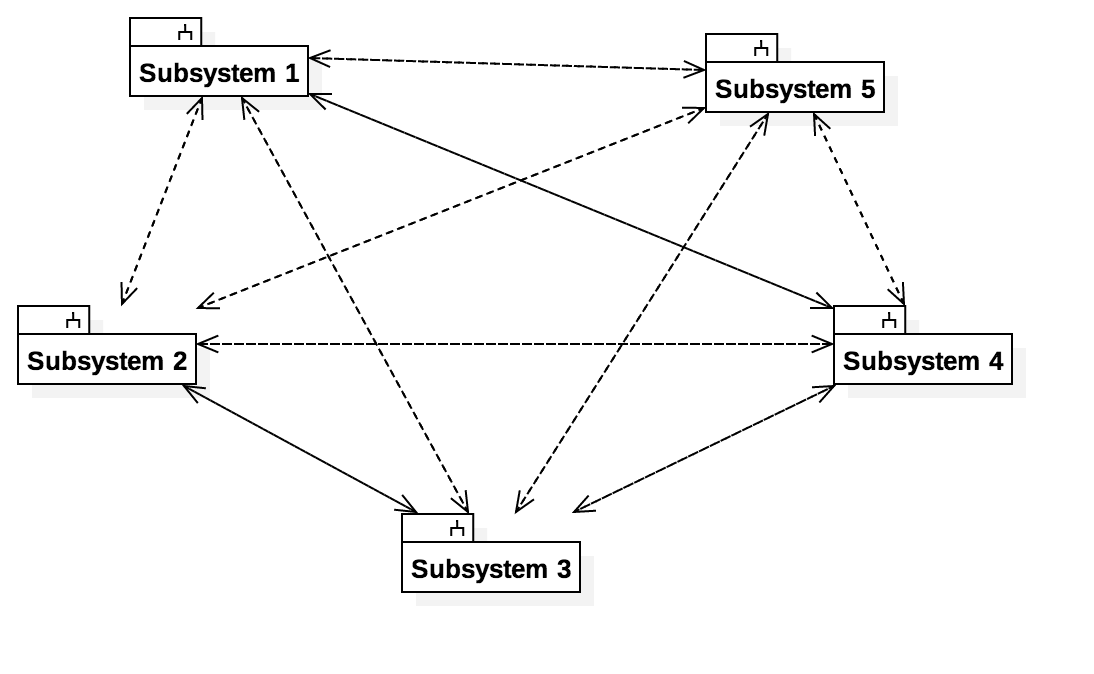
\includegraphics[width=15cm]{otros/UML/png/arquitectura_mala.png}
	\caption{Arquitectura con subsistemas interconectados directamente}
	\label{dia:arquitectura_mala}
\end{figure}

\bigskip

Aquí es donde entra la arquitectura basada en subsistemas conectados por el bus de mensajes que permite evitar las múltiples referencias y controlar con mucha más facilidad las comunicaciones dentro de la aplicación. En la figura \ref{dia:arquitectura_general} se observa la diferencia en términos de simplicidad y orden.

\bigskip

\begin{figure}
	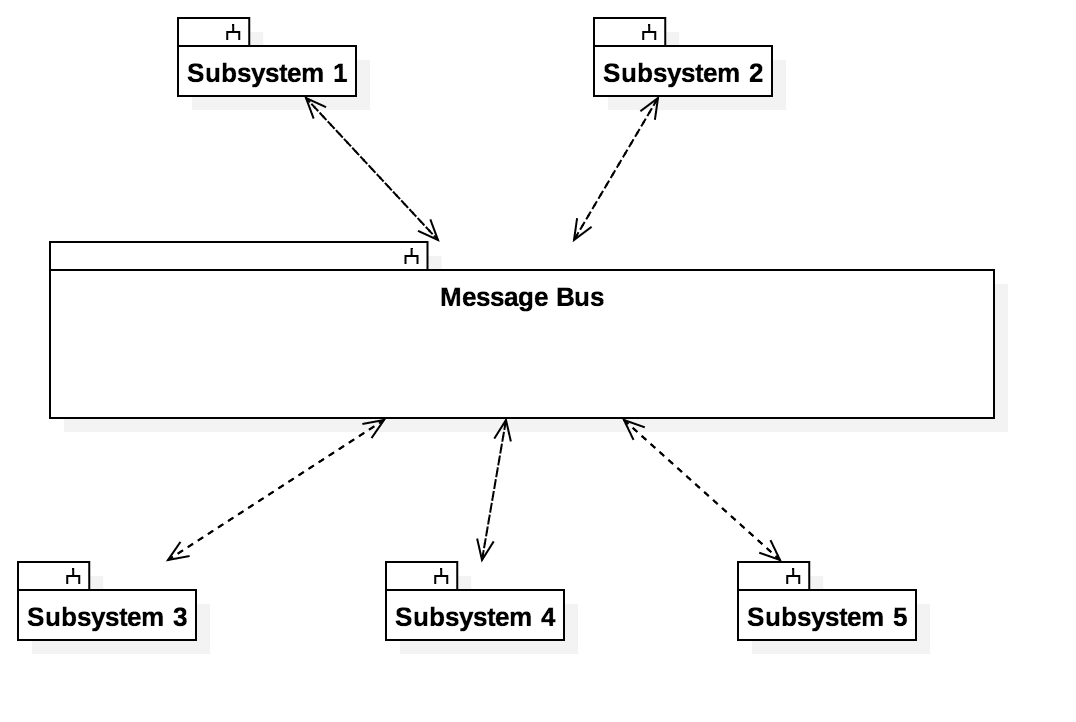
\includegraphics[width=15cm]{otros/UML/png/arquitectura_general.png}
	\caption{Arquitectura con subsistemas interconectados mediante bus de mensajes}
	\label{dia:arquitectura_general}
\end{figure}

\bigskip

De hecho, sobre la arquitectura general mostrada en la figura \ref{dia:arquitectura_general} se harán una serie de modificaciones de forma que todos los subsistemas sean totalmente transparentes a ojos del bus de mensajes. Para ello se hará que los mismos hereden de lo que llamaremos un \textit{Bus Node} o nodo del bus. La forma que tendría esta arquitectura de forma genérica es la mostrara en la figura \ref{dia:actual_arquitecture}

\bigskip

\begin{figure}
	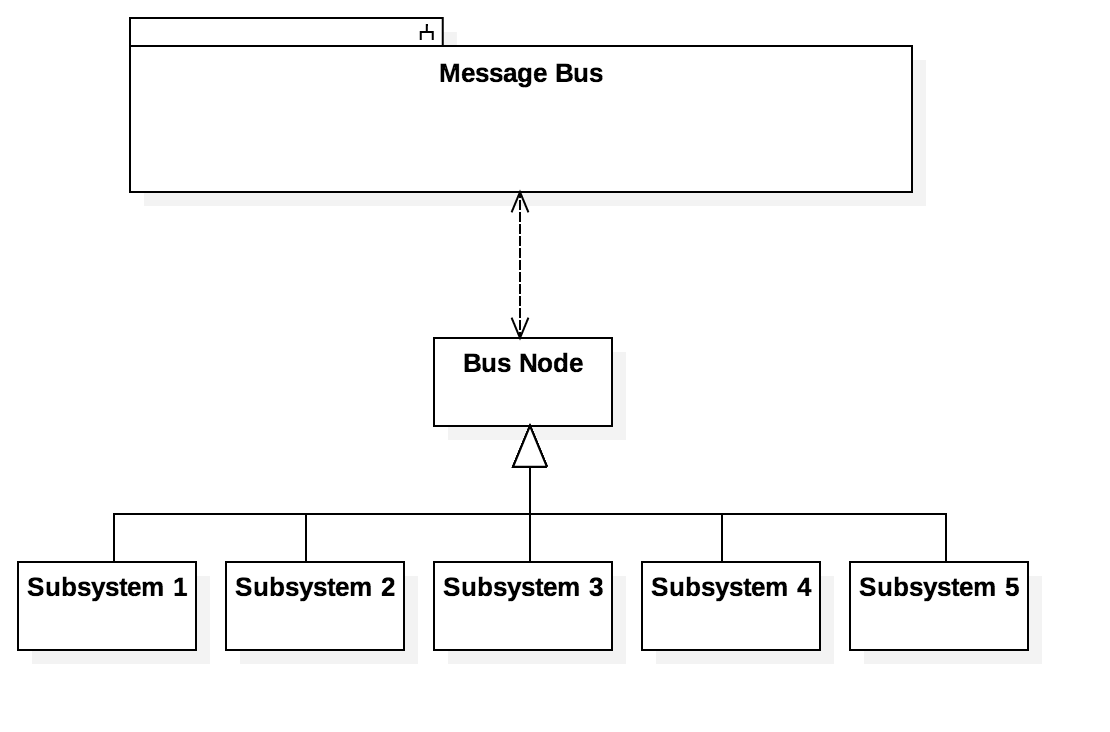
\includegraphics[width=15cm]{otros/UML/png/actual_arquitecture.png}
	\caption{Arquitectura con Bus Node}
	\label{dia:actual_arquitecture}
\end{figure}

\bigskip

Sobre esta arquitectura general se realizará una modificación relacionada con el requisito no funcional RNF-4 para facilitar los procesos de depuración de errores. Dado que todos los mensajes pasarán por el bus de mensajes se podrá hacer que los mismos sean mostrados en la consola interna de la aplicación o incluso introducir mensajes en forma de comandos en dicha consola. Para hacer esto posible se necesitará tratar de modo especial la consola como subsistema de forma que la arquitectura final será la que se puede ver en la figura \ref{dia:arquitectura_final}.

\bigskip

\begin{figure}
	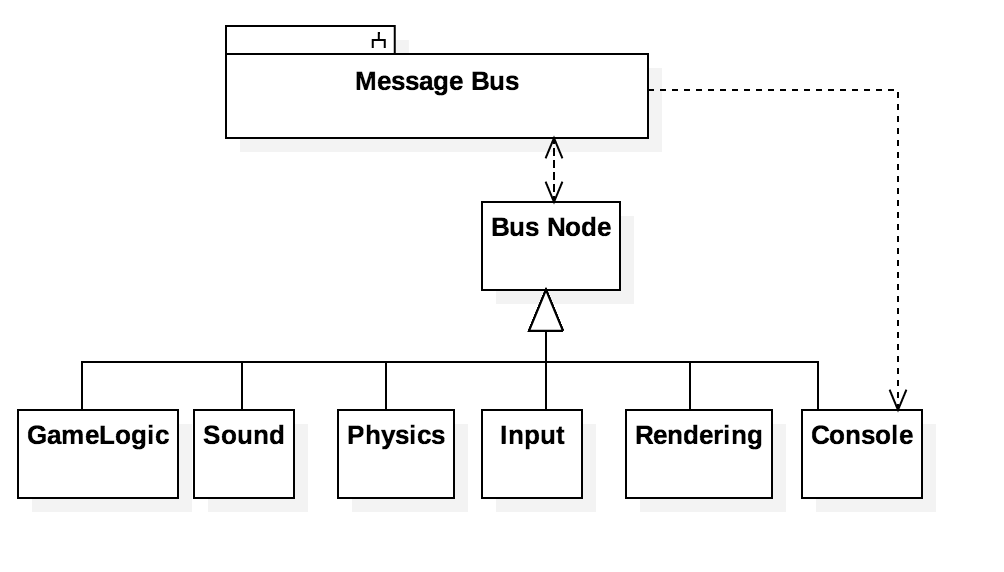
\includegraphics[width=15cm]{otros/UML/png/final_arq.png}
	\caption{Arquitectura final}
	\label{dia:arquitectura_final}
\end{figure}

\bigskip

También podemos observar en la figura \ref{dia:arquitectura_final} el componente que representa la lógica del juego es la que ocasionará que se ejecuten las diferentes funcionalidades de una forma u otra. Como \textit{GameLogic} se entiende a todas las clases dedicadas a definir los datos y comportamiento del videojuego en un determinado estado, por ejemplo, la lógica de un menú contendrá las opciones disponibles con la acción que corresponde a cada una de ellas, además tendrá la funcionalidad de cambiar entre las mismas y seleccionar la que se desee.

\bigskip

\subsection{Subsistemas propios del motor}

En relación a la figura \ref{dia:arquitectura_final} se dedicará este apartado a explicar la función general de cada uno de los subsistemas que no componen la lógica de la aplicación o \textit{GameLogic}.

\begin{itemize}
	\item \textbf{\textit{Sound} o Sonido}: Será el subsistema encargado de reproducir cualquier tipo de sonido que necesite la aplicación, desde pequeñas indicaciones que confirman que se ha cambiado de opción en el menú hasta el sonido de realizar un ataque, incluyendo música si se fuera a añadir.
	\item \textbf{\textit{Physics} o Físicas }: Será el subsistema encargado de lidiar con todas las funcionalidades relacionadas con la simulación de físicas en la aplicación. Esto puede incluir detectar colisiones contra muros y evitar que se puedan atravesar o detectar cuando un ataque realizado por un personaje ha alcanzado al otro o no.
	\item \textbf{\textit{Input} o Entrada}: Será el subsistema que recibirá todas las entradas realizadas por el usuario, desde teclas pulsadas hasta movimientos de un joystick, para luego enviárselas a los otros subsistemas para que gestionen si deben ejecutar algún proceso.
	\item \textbf{\textit{Rendering} o Renderizado}: Será el subsistema encargado de mostrar cualquier tipo de gráficos por pantalla. Necesitará gestionar la ventana y todas sus acciones (cambiar el tamaño, cerrarla, etc.) Además contendrá la funcionalidad de mostrar las animaciones realizadas, texto, efectos, etc.
	\item \textbf{\textit{Console} o Consola}: Será el subsistema utilizado para ver los mensajes importantes de la aplicación así como enviar mensajes en forma de comandos introducidos en tiempo de ejecución. Será la interfaz que el usuario tendrá para introducir mensajes directamente en el bus de mensajes.
\end{itemize}
  

\section{Herramientas de diseño}

Los modelos formales mostrados en esta memoria utilizan UML o \textit{Unified Modeling Language}. En términos de lenguajes de modelado para software este es sin duda el estándar más expandido, soportado además por el OMG\footnote{\textit{Object Management Group}: Consorcio dedicado a establecer y gestionar estándares relacionados con el paradigma de la orientación a objetos}/

\bigskip

Pese a que el lenguaje completo en su versión 2.5 ofrezca 14 tipos de diagramas específicos, en esta memoria se han utilizado solamente 4, siendo los mismos:

\begin{itemize}
	\item \textbf{Diagrama de casos de uso}: Dedicado a modelar el comportamiento del sistema ante los actores que interactúan con él.
	\item \textbf{Diagrama de paquetes}: Utilizado para mostrar los subsistemas y componentes genéricos de la aplicación.
	\item \textbf{Diagrama de clases}: Usados para definir y especificar las diferentes clases de cada subsistema y las relaciones entre las mismas.
	\item \textbf{Diagrama de secuencia}: Que modelan los casos de uso definidos en términos de la interacción entre objetos de la aplicación.
\end{itemize}

\subsection{Herramientas software}

Relacionado con el diseño solo se ha utilizado una aplicación concreta siendo la misma el \textit{StarUML 2.8}\footnote{http://staruml.io/}. La elección surgió a raíz de históricamente que ha sido la seleccionada para modelar durante la carrera y no se han experimentado deficiencias en términos de funcionalidades que implicaran tener que buscar un sustituto.

\subsection{Patrones de diseño}

Al trabajar con el paradigma de orientación a objetos es muy común que, si se diseña o programa sin prestar atención a las necesidades de la aplicación y sin considerar lecciones aprendidas anteriormente, se llegue a una situación en la cual se ha desarrollado una solución extremadamente compleja para un problema relativamente simple. A muy alto nivel, las lecciones aprendidas por parte de toda la comunidad de programadores y diseñadores se representan en forma de \textbf{patrones de diseño}.

\bigskip

Un patrón de diseño representa una solución a un problema común y genérico que ha sido generada y probada a partir de su uso continuado por parte de la comunidad. Lo que aporta esto es la flexibilidad de aplicar soluciones con la seguridad de estar utilizando modelos simples y potentes que no generarán errores en el diseño si se usan correctamente. Además, su implementación se hace significativamente más sencilla ya que la documentación y recursos disponibles para aprender a codificarlos está muy extendida.

\bigskip

En las siguientes secciones de este apartado se muestran los patrones utilizados de forma consciente en la aplicación ya que es relativamente común que debido a la práctica se lleguen a diseños que contienen patrones sin haberse propuesto implementarlos.

\bigskip

\subsubsection{Patrón \textit{Strategy}}

Para la implementación de comportamientos diferentes del enemigo nos será de mucha utilidad el patrón \textit{Strategy}  ya que el mismo está enfocado a cambiar los algoritmos que definen el comportamiento de un objeto de forma dinámica. De esta forma se puede cambiar fácilmente entre el enemigo controlado por el agente o el controlado por reglas siendo esto transparente al personaje que está siendo controlado.

\bigskip

Este patrón aporta una serie de ventajas relevantes para nuestro caso que son las siguientes:

\begin{itemize}
	\item No se tiene que agregar el código de los algoritmos al cliente (personaje) ya que el mismo puede ser muy complejo.
	\item El cliente no necesita todos los algoritmos en todas las situaciones por lo que evitamos que sea él el que los almacene.
	\item Si existen varios clientes que utilicen los mismos algoritmos se evita duplicar el código.
\end{itemize}

\bigskip

En la figura \ref{pat:strategy} se observa una definición genérica del patrón donde las diferentes partes son:

\begin{itemize}
	\item \textbf{\textit{Context}}: La clase que contendrá a la estrategia sea cual sea la misma. Esto puede ser el propio cliente o puede estar contenida en él.
	\item \textbf{\textit{Strategy}}: Clase abstracta que representa a una estrategia genérica, por si misma no contiene comportamiento alguno.
	\item \textbf{\textit{ConcreteStrategy}}: Clase que implementa cada uno de los diferentes comportamientos entre los que se puede cambiar.
\end{itemize}

\bigskip

\begin{figure}
	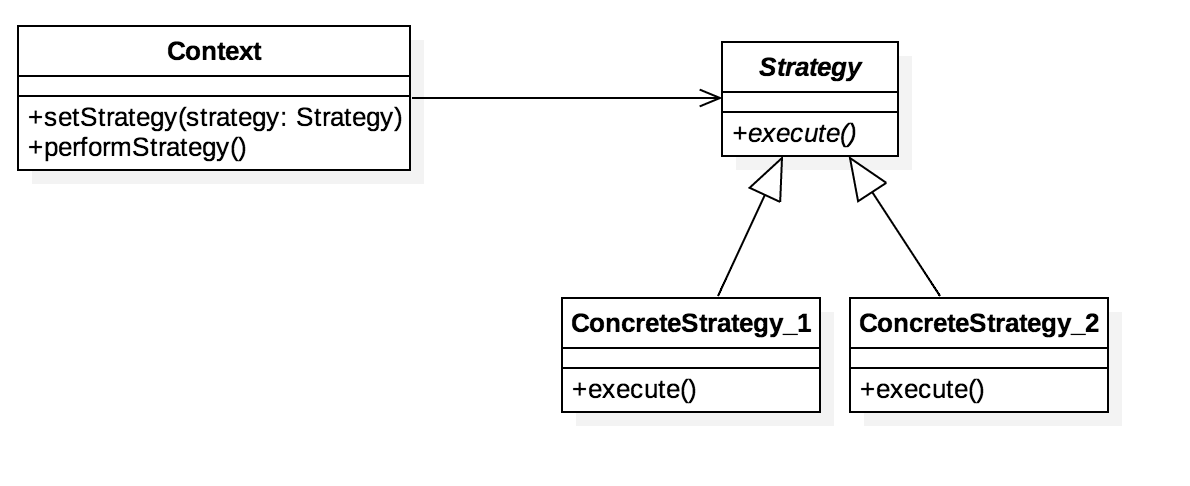
\includegraphics[width=15cm]{otros/UML/png/strategy.png}
	\caption{Patrón \textit{Strategy}}
	\label{pat:strategy}
\end{figure}


\subsubsection{Patrón \textit{Singleton}}

A la hora de requerir que solo exista una instancia de un componente concreto en una ejecución del programa el patrón a utilizar es el conocido como \textit{Singleton}. Este patrón permite además hacer que ese componente sea accesible por cualquier otro con facilidad, algo comúnmente necesario en videojuegos ya que hay entidades como gestores de recursos, relojes o sistemas de colisiones que deben ser comunes y únicos.

\bigskip

Estas dos ventajas comentadas son las que han decantado la balanza a favor de su elección. Sin embargo se debe tener mucho cuidado con el uso de este patrón ya que puede suponer una refactorización de código muy importante si luego se decide que el objeto no debe de tener acceso global o que se necesitan varias instancias del mismo.

\bigskip

\begin{figure}
	\centerline{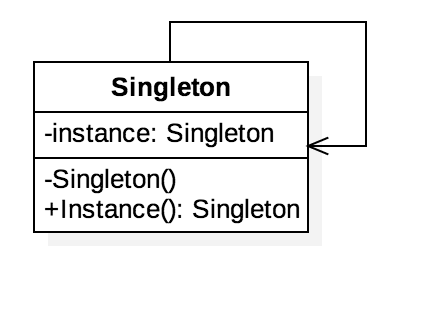
\includegraphics[width=5cm]{otros/UML/png/singleton.png}}
	\caption{Patrón \textit{Singleton}}
	\label{pat:singleton}
\end{figure}

\bigskip

En la figura \ref{pat:singleton} podemos ver el único componente que conforma el patrón. Esta clase tiene un método \textit{Instance()} que permite acceder a la única instancia que existe. Dicha instancia o \textit{instance} es privada, de la misma que el constructor \textit{Singleton()} para evitar así que se creen nuevos objetos desde fuera.


\subsubsection{Patrón \textit{Decorator}}

Cuando se necesita extender la funcionalidad de un objeto de forma dinámica el patrón más comúnmente usado es el conocido como \textit{Decorator}. El mismo permite agregar componentes a un objeto de forma que los mismos puedan contener operaciones o estado adicionales. En el contexto de un videojuego suele ser necesario que la escena en la que se trabaje y los objetos que están en ella se puedan gestionar de forma dinámica. Se explicará más en detalle en el apartado de diseño e implementación.

\bigskip

\begin{figure}
	\centerline{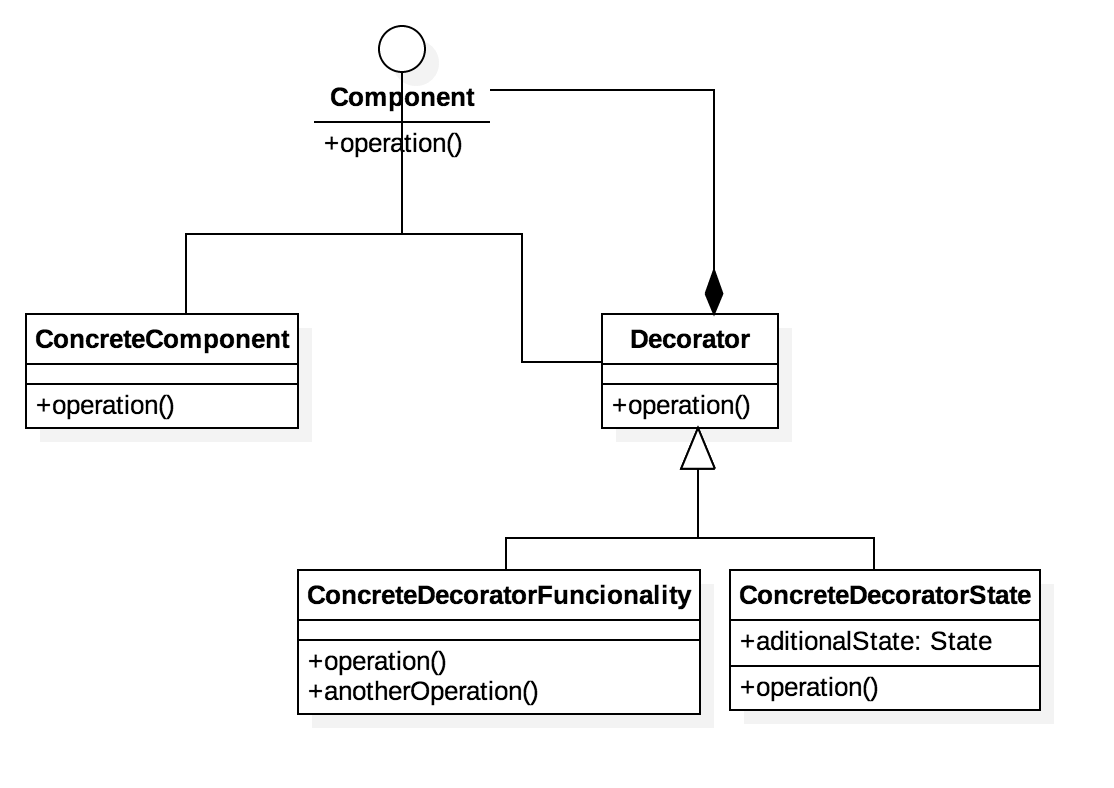
\includegraphics[width=12cm]{otros/UML/png/decorator.png}}
	\caption{Patrón \textit{Decorator}}
	\label{pat:decorator}
\end{figure}

\bigskip

En la figura \ref{pat:decorator} se ven los diferentes componentes que cuentan con las siguientes responsabilidades:

\begin{itemize}
	\item \textbf{\textit{Component}}: Interfaz para los objetos que pueden recibir nuevas responsabilidades dinámicamente.
	\item \textbf{\textit{ConcreteComponent}}: Objeto que puede recibir responsabilidades adicionales de forma dinámica.
	\item \textbf{\textit{Decorator}}: Referencia al objeto componente definiendo la interfaz que se ajusta a la interfaz del componente.
	\item \textbf{\textit{ConcreteDecorator}}: Extienden el componente añadiendo funcionalidad y/o estado.
\end{itemize}

\subsubsection{Patrón Publica-Subscribe o \textit{PubSub}}

El patrón Publica-Subscribe se utiliza cuando es necesario que diversos objetos reciban ciertos mensajes en los que pueden estar interesados mientras otros son los encargados de generar dichos mensajes. Esto se dá en el caso del  bus de mensajes ya que los diferentes subsistemas están interesados en recibir los mensajes relevantes para ellos.

\bigskip

\begin{figure}
	\centerline{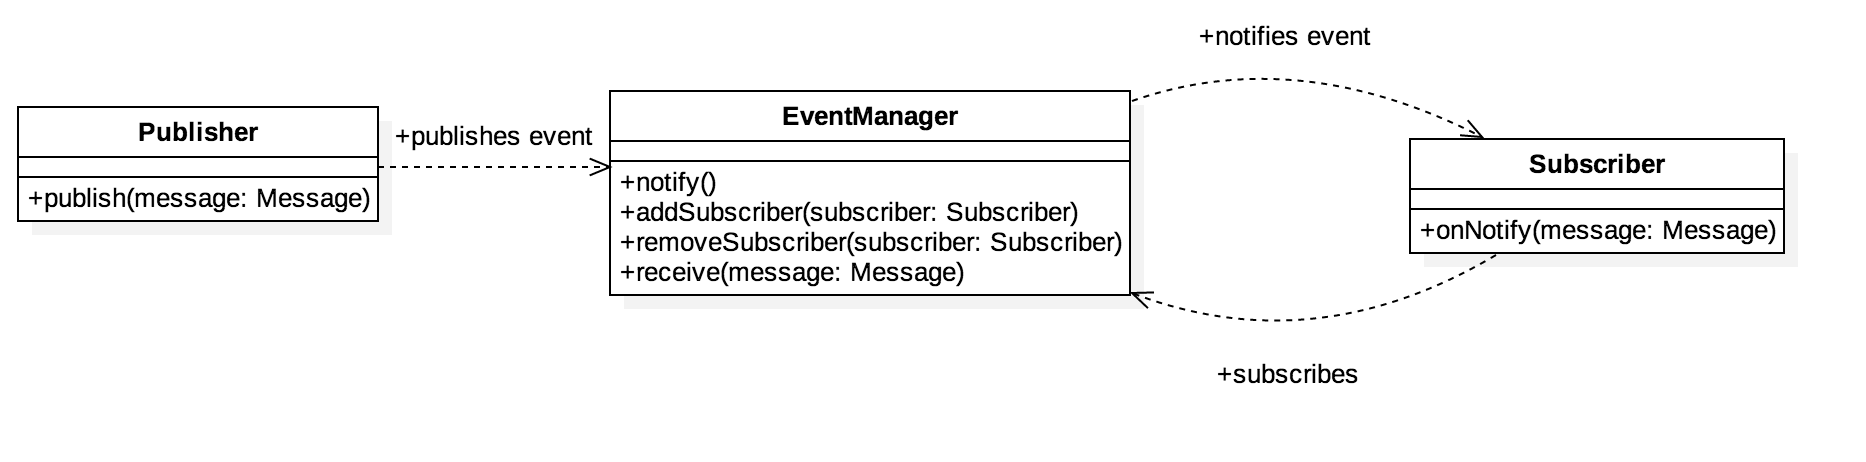
\includegraphics[width=18cm]{otros/UML/png/pubsub.png}}
	\caption{Patrón Publica-Subscribe o \textit{PubSub}}
		\label{pat:pubsub}
\end{figure}

\bigskip
 
En la figura \ref{pat:pubsub} se pueden observar los componentes del patrón que realizan las siguientes funciones:

\begin{itemize}
	\item \textbf{\textit{Publisher}}: Objeto que genera los mensajes y los envía al \textit{EventManager}.
	\item \textbf{\textit{EventManager}}: Objeto que recibe los mensajes y los distribuye a los subscriptores, además permite agregar o quitar subscriptores de forma dinámica.
	\item \textbf{\textit{Subscriber}}: Objeto encargado de subscribirse que luego recibirá los mensajes por parte del \textit{EventManager}.
\end{itemize}

\bigskip

Tenemos que comentar que en la aplicación, como se ve en el apartado de diseño, se realizará una aproximación ligeramente diferente en la cual todos los subsistemas publican y reciben mensajes. Estas dos responsabilidades estarán asociadas al \textit{BusNode} que es el que se conectará con el bus de mensajes que representa al \textit{EventManager}.


\section{Herramientas de desarrollo}

La elección de las herramientas de desarrollo utilizadas en este proyecto ha estado significativamente influenciada por el conocimiento previo que se tenía de las mismas. Esta práctica es habitual en todos los proyectos pero se vuelve más necesaria aún cuando el tiempo disponible para realizar el proyecto está limitado.

\bigskip

En este sentido, prácticamente siempre que se pudo elegir una herramienta conocida para realizar alguna tarea se ha escogido. Dicho esto, el entorno de desarrollo a rasgos muy generales que se ha utilizado está compuesto por las siguientes herramientas:

\bigskip

\begin{itemize}
	\item \textbf{Sistema operativo}: macOS Sierra 10.12.5
	\item \textbf{Compilador}: clang 802.0.42 (basado en Apple LLVM 8.1.0)
\end{itemize}

\bigskip

El entorno es relativamente  corto y fácil de describir dada la ausencia de bases de datos o frameworks que corran por encima del lenguaje utilizado. Pese a que en la lista anterior solo se mencionen el sistema y compilador utilizados, se entrará en detalle sobre las herramientas específicas dedicadas a la elaboración de la documentación, el desarrollo del código, las tecnologías elegidas y las librerías utilizadas.

\subsection{Realización de la documentación}

Para generar la documentación del proyecto y, por lo tanto, esta misma memoria se han utilizado las siguientes herramientas:

\begin{itemize}
	\item \textbf{TeXstudio\footnote{http://www.texstudio.org/}}: La elección de este editor para archivos .tex se ha escogido dado su amplio uso en la comunidad, la cantidad y calidad de la documentación del mismo y el hecho de que es soportado en todos los sistemas operativos importantes, lo que reduce el riesgo de tener que utilizar otra herramienta si ocurren problemas con el equipo de desarrollo.
	\item \textbf{Microsoft Project 2013}: Gracias a las versiones de prueba que ofrece Microsoft para este software se ha podido utilizar esta herramienta. Teniendo la opción de elegir entre las diferentes opciones orientadas a la gestión de proyectos la mejor sin duda es Project. Aporta muchas más facilidades y posibilidades que los competidores y es el estándar de facto. Además, si las versiones de prueba dejan de estar disponibles, muchas de las otras herramientas soportan la importación de proyectos de Microsoft Project, posibilitando así continuar con el proyecto.
	\item \textbf{StarUML 2.8}: Usado tanto para elaborar los diagramas como para exportarlos a imágenes integrables en la documentación. Como 
\end{itemize}


\subsection{Desarrollo}

Las herramientas que han sido necesarian para llevar a cabo la implementación de la aplicación han sido las siguientes:

\begin{itemize}
	\item Motor \textbf{Unity 5}: Se escogió como herramienta principal para desarrollar la aplicación hasta que se descubrieron las limitaciones mencionadas en la acción correctiva AC-1. La elección inicial estaba fundamentada en las facilidades que otorga para implementar aplicaciones de este tipo y la consecuente velocidad a la hora de obtener versiones funcionales rápidamente.
	\item IDE \textbf{MonoDevelop}: Necesario para trabajar con el código en C\# que utiliza Unity en macOS. Pese a que sea un IDE simplemente se utilizaba para la edición de código dadas las facilidades a la hora de detectar errores en el mismo.
	\item IDE \textbf{Xcode 8.3.3}: Al estar estrechamente integrado con el sistema de Apple nos permite realizar todo el desarrollo en un mismo entorno. Automáticamente busca y utiliza las herramientas por defecto a la hora de detectar errores en el código, compilar, depurar y empaquetar la aplicación. Además integra un potente \textit{profiler} que ayuda a detectar los cuellos de botella de la aplicación, algo muy importante en situaciones como esta en la que el rendimiento es importante.
	\item Compilador \textbf{clang-802.0.42 basado en Apple LLVM 8.1.0}: La elección de este compilador era clara, además de soportar las especificaciones de C++ necesarias (completamente hasta C++14) también puede compilar código escrito en Objective C, ya que se ha requerido para una pequeña parte relacionada con el empaquetado de la aplicación. Este compilador es automáticamente utilizado por Xcode por lo que a ojos del usuario es completamente transparente.
\end{itemize}

\subsection{Tecnologías}

Las tecnologías que se incluyen en este apartado están compuestas por los diferentes lenguajes de programación escogidos para cada una de las partes, así como de cualquier otro tipo de lenguaje que se haya tenido que utilizar.

\begin{itemize}
	\item \textbf{C\#}: Elegido porque es el lenguaje que utiliza Unity para correr los diferentes archivos o \textit{scripts} que definen el comportamiento de los objetos del juego.
	\item \textbf{C++}: Dada la relativa experiencia que el desarrollador tenía en este lenguaje se consideró el mismo una buena opción para el proyecto. Más incluso cuando se consideró que el rendimiento era importante dado que la ausencia de un \textit{runtime} encargado de correr nuestro código, realizar recolección de basuras, etc podía ser catastrófico a la hora de conseguir la velocidad de simulación deseada. Además, en términos de lenguajes compilados a bajo nivel C++ es el que más se ajustaba al paradigma orientado a objetos.
	\item \textbf{Objective-C}: Extensión de C orientada a objetos similar a C++ pero utilizado principalmente en sistemas Apple. Nos ha permitido encapsular todos los archivos y recursos de la aplicación en un mismo ejecutable, haciendo el producto final extremadamente portable en todos los sistemas macOS. 
	\item \textbf{JSON}: Formato de texto orientado a la transmisión y representación de datos de forma ligera. Se ha utilizado para escribir los datos referentes a las animaciones para así saber que imagen se debe mostrar, en que orden y durante cuanto tiempo. 
\end{itemize}

\subsection{Librerías}

Finalmente, las librerías utilizadas simplemente se referirán a las que son llamadas desde el código C++ pues los otros lenguajes no requerían extensión alguna para realizar las funcionalidades que se implementaron con ellos.

\begin{itemize}
	\item \textbf{Biblioteca estándar de C++}: Básica a la hora de trabajar con C++ ya que soporta los contenedores genéricos y funcionalidades asociadas más utilizados en el lenguaje a la vez que completa las características del mismo al soportar funcionalidades en entrada y salida a archivos o salida estándar. 
	\item \textbf{SFML}: Librería a bajo nivel que sirve como interfaz sobre OpenGL. Gestiona la creación de ventanas en el sistema operativo que se requiera y ofrece funcionalidades útiles a la hora de mostrar por pantalla, reproducir sonidos, etc.
	\item \textbf{json.h}: Librería en formato de cabecera única que sirve para facilitar la lectura y escritura de archivos json. Disponible en GitHub\footnote{https://github.com/sheredom/json.h} en la cuenta de su creador, \textit{sheredom}, el cual la proporciona sin requerir ningún tipo de licencia.
	\item \textbf{Boost}: Conjunto de bibliotecas de software libre enfocadas a extender al lenguaje C++ con funcionalidades comúnmente necesitadas como realización de operaciones algebraicas complejas, procesamiento de imágenes, expresiones regulares o nuevos tipos de datos.
\end{itemize}


\cleardoublepage
\chapter{Diseño e implementación}
\label{cap:diseno}
En este capítulo se documenta el diseño e implementación que se ha realizado para dar lugar a la aplicación final. Como bien se explica en el capítulo dedicado a la arquitectura, se ha seguido una división por subsistemas por lo que la mejor aproximación para separar ahora los múltiples diagramas de clases es hacerlo por paquetes, asociados cada uno de ellos a un subsistema. Además se generarán una serie de paquetes que contienen una serie de funcionalidades adicionales utilizadas por los otros.

\bigskip

Se empezará por la documentación asociada a los paquetes relacionados con el motor del videojuego en sí mismo para luego seguir con el subsistema de la lógica de la aplicación que contendrá la implementación del agente. Luego se muestran los diagramas de interacción que relacionan las clases antes definidas con los casos de uso en los que participan. Finalmente se mostrará como se llegó al diseño de la interfaz gráfica de la aplicación. Además, se ha hecho uso de un \textbf{código de colores} que permite una comprensión más rápida de cada uno de los diagramas:

\begin{itemize}
	\item \textbf{Verde}: Identifica las clases protagonistas o principales de cada diagrama.
	\item \textbf{Morado}: Identifica las clases que ayudan a las principales a realizar la función que se les requiere, estas clases \textbf{pertenecen} al paquete/diagrama que se está mostrando.
	\item \textbf{Amarillo}: Identifica las clases que son necesarias para llevar a cabo las funcionalidades del paquete/subsistema pero que \textbf{no pertenecen} al mismo.
	\item \textbf{Azul}: Identifica las clases, estructuras o enumeraciones que representan contenedores de datos sin funcionalidades complejas.
\end{itemize}

\section{Diagramas de clases}

Para facilitar la comprensión de la estructura de esta sección la misma está ordenada de la siguiente forma:

\begin{enumerate}
	\item Primero se explicará la estructura asociada al bus de mensajes.
	\item Luego se mostrará la estructura genérica de la aplicación con todos los subsistemas.
	\item Se explicarán los subsistemas individualmente.
	\item Brevemente, se mencionarán algunas clases adicionales.
	\item Finalmente se mostrarán los diagramas de cada una de las escenas.
\end{enumerate}

En los apartados que siguen se añadirá una breve explicación asociada a cada diagrama para favorecer su comprensión.  Además, en aras de mantener la simplicidad de los diagramas, se han omitido los constructores que no aportan información sobre la clase, es decir, si una clase no requiere argumentos o requiere los mismos que una superclase no se mostrará su constructor. En situaciones donde sea relevante como que requiera argumentos inesperados o el constructor sea privado se especificará como tal.

\subsection{Bus de mensajes}

\begin{figure}
	\centerline{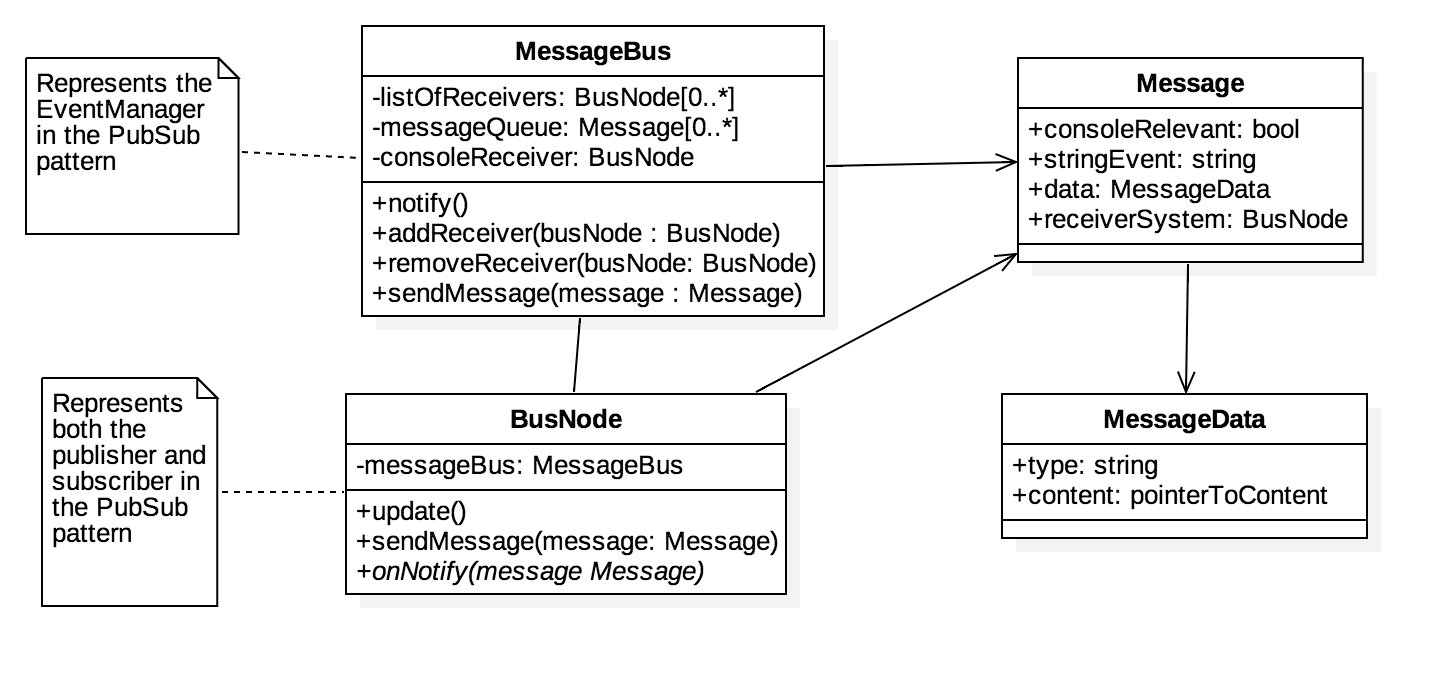
\includegraphics[width=15cm]{otros/UML/png/alld/png/messaging__diagramaDeClases_messaging_11.png}}
	\caption{Diagrama de clases del bus de mensajes}
	\label{class:messageBus}
\end{figure}

En la figura \ref{class:messageBus} se encuentra el diagrama de clases del bus de mensajes, en el mismo se vé implementada una modificación del patrón \textit{PubSub} (mostrado en la figura \ref{pat:pubsub}) en la cual la clase \textbf{\textit{BusNode}} representa tanto a los publicadores como a los subscriptores. Dicha clase es la encargada de encapsular las funcionalidades asociadas a enviar y recibir mensajes por parte de cada subsistema.

\bigskip

Por otra parte, la clase \textbf{\textit{MessageBus}} es la que representa el \textit{EventManager} del patrón \textit{PubSub}. La misma es la encargada de almacenar los mensajes y enviarlos a todas las instancias de \textit{BusNode} que lo requieran.

\bigskip

Finalmente, se ven las clases \textbf{\textit{Message}} y \textbf{\textit{MessageData}} que representan los mensajes que se envía y su contenido.

\subsection{Aplicación general}

\begin{figure}
	\centerline{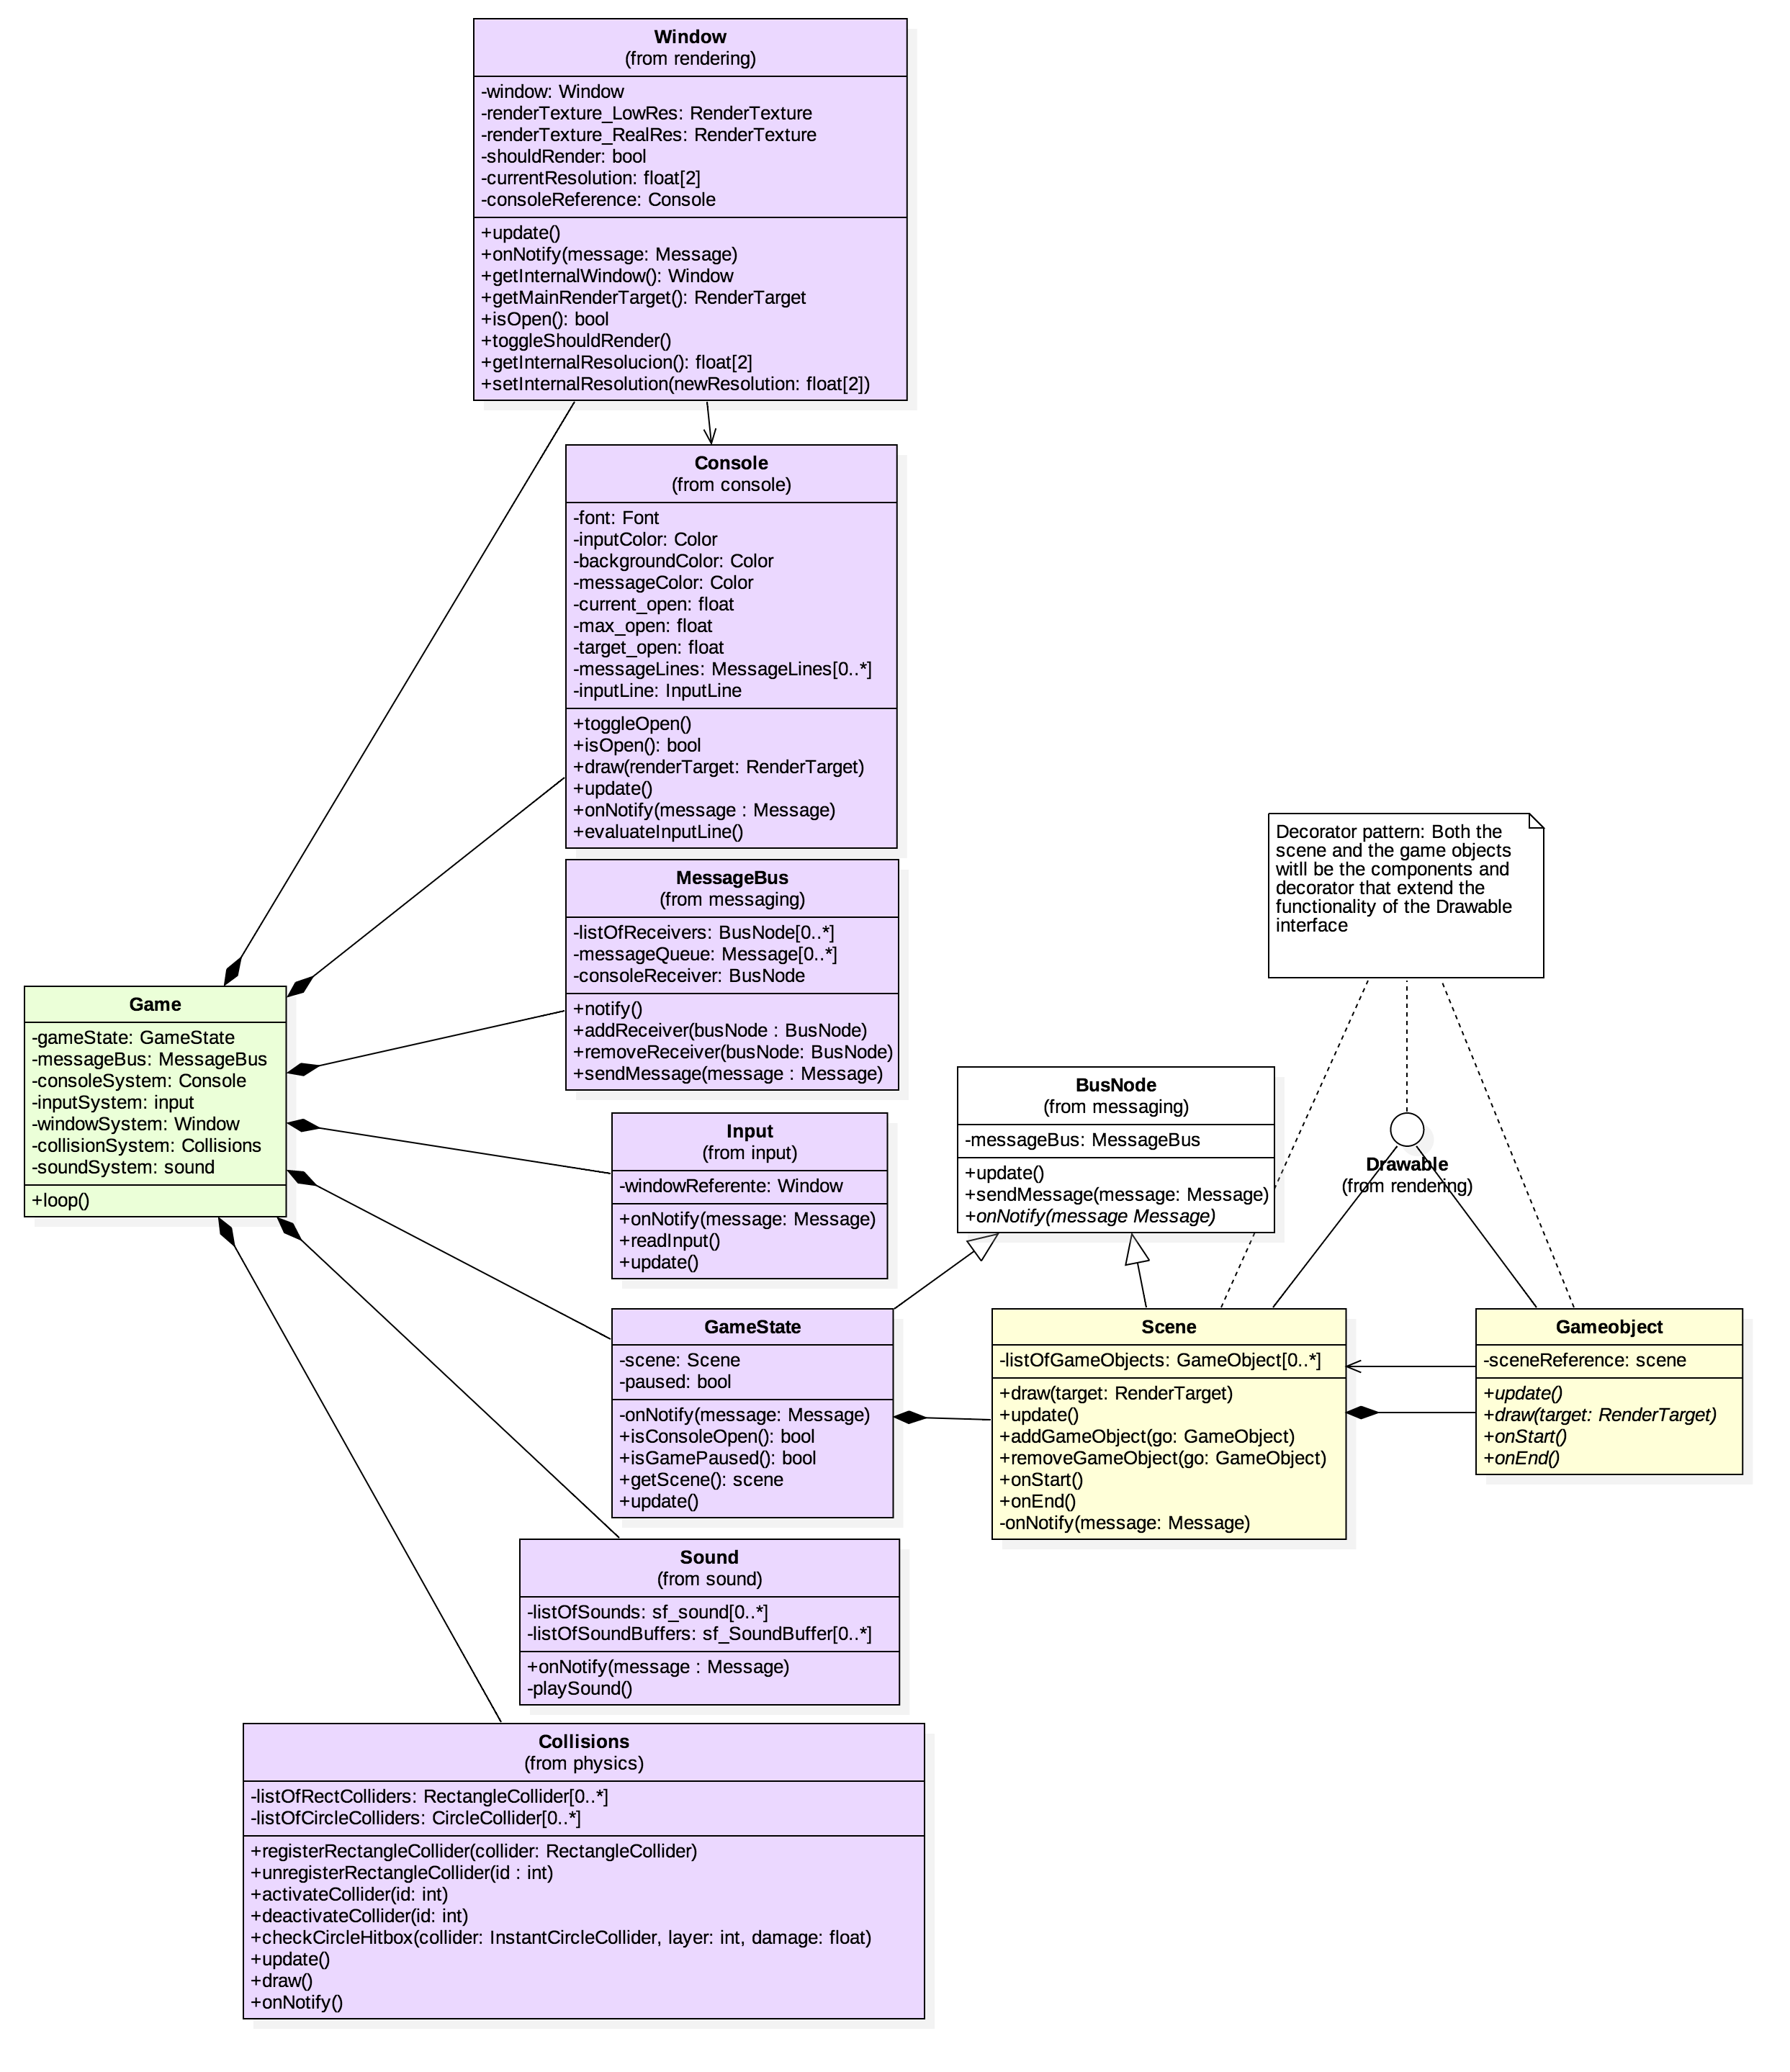
\includegraphics[width=18cm]{otros/UML/png/alld/png/gamelogic__diagramaDeClases_gamelogic_7.png}}
	\caption{Diagrama de clases de la lógica del juego}
	\label{class:gamelogic}
\end{figure}

La figura \ref{class:gamelogic} contiene la lógica del juego mostrada a muy alto nivel. La clase principal es \textbf{\textit{Game}} que es instanciada en el \textit{main} de la aplicación. La misma contiene la función \textit{loop} que simplemente itera por todos los subsistemas, actualizándolos, como se ve en el diagrama de secuencia \ref{sec:general}. 

\bigskip

También se observan las clases asociadas a cada uno de los subsistemas, muy importante es la clase \textbf{\textit{GameState}} que contiene a la escena de la aplicación representada por la clase \textbf{\textit{Scene}}. Aquí podemos ver el patrón \textit{Decorator} (Figura \ref{pat:decorator}) en el cual la escena y los \textit{gameobjects} (representados en la clase \textbf{\textit{GameObject}}) agregan estado y funcionalidad. Cada \textit{gameobject} representa uno de los objetos pertenecientes a la escena desde el punto de vista del juego a alto nivel, esto puede ser un personaje, texto, una barra de vida, un contador de tiempo, etc.


\subsection{Subsistemas}

\subsubsection*{Subsistema de consola}

\begin{figure}
	\centerline{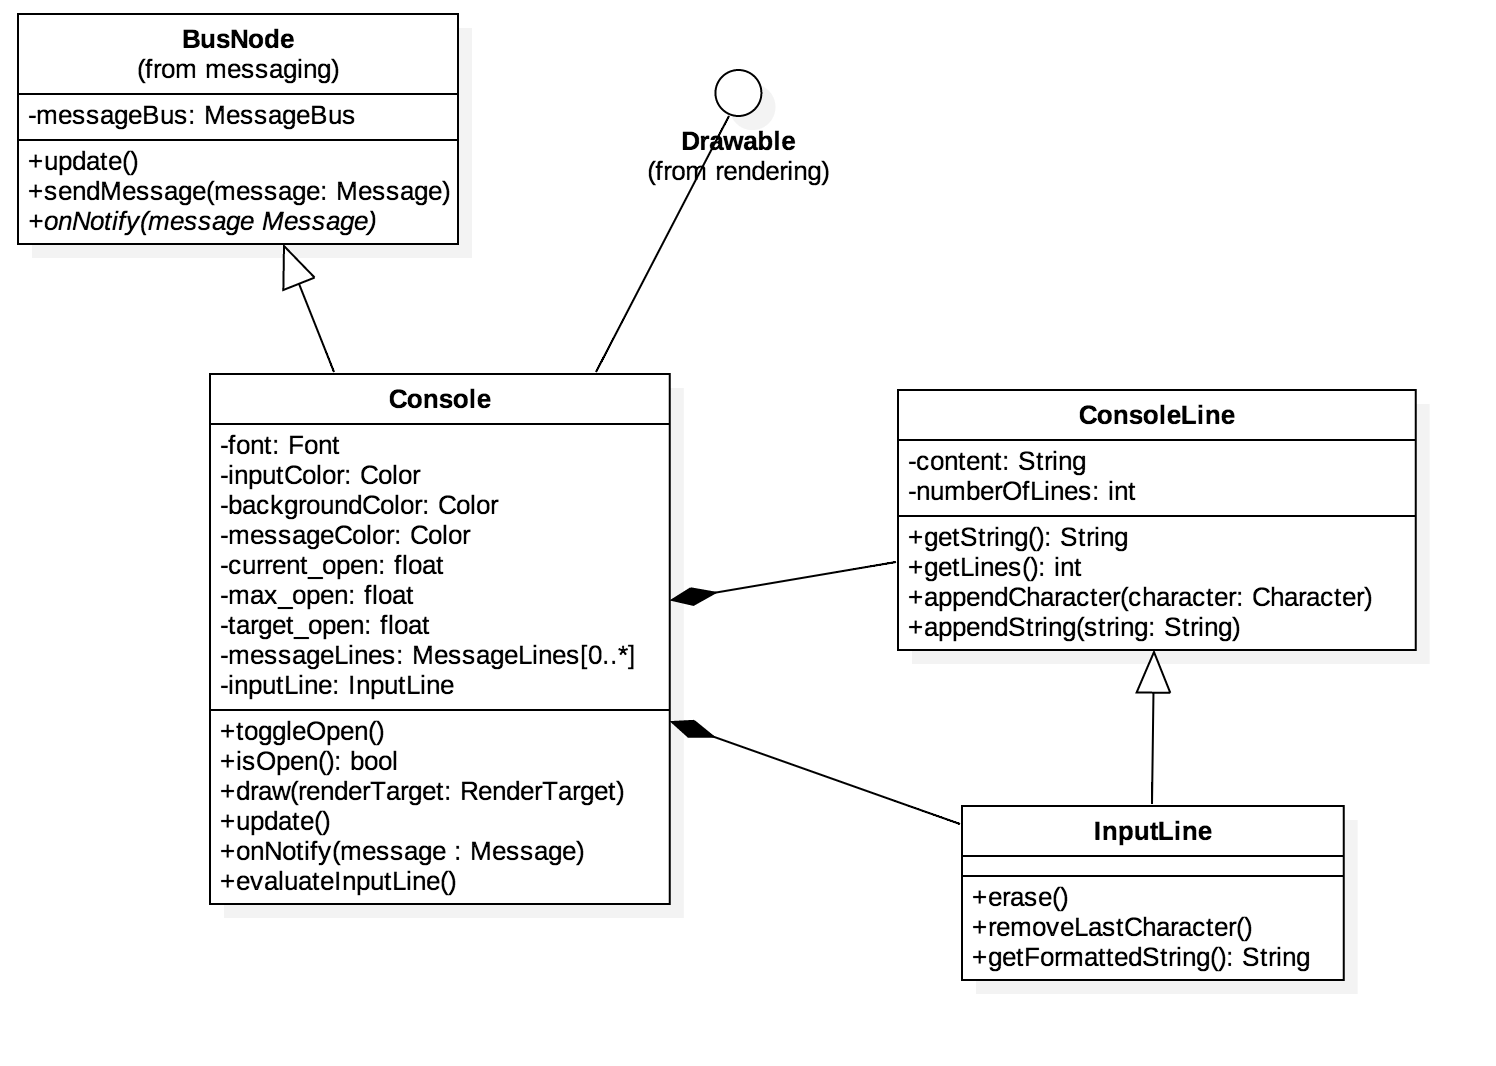
\includegraphics[width=15cm]{otros/UML/png/alld/png/console__diagramaDeClases_console_3.png}}
	\caption{Diagrama de clases del subsistema de consola}
	\label{class:console}
\end{figure}

En la figura \ref{class:console} se ven las clases que componen el subsistema de la consola. En el mismo, la clase \textbf{\textit{Consola}} es la que contiene todas las funcionalidades necesarias, como abrirse y cerrarse con el método \textit{toggleOpen}, ser dibujada con el método \textit{draw} o evaluar la cadena de texto introducida con \textit{evaluateInputLine}.

\bigskip

Vemos además la jerarquía de \textit{ConsoleLine} e \textit{InputLine}. Se encargan respectivamente de contener todas las lineas de texto a mostrar en la consola y de contener el texto introducido por el usuario. \textit{InputLine} extiende a \textit{ConsoleLine} en el sentido de que agrega las funcionalidades necesarias para agregar texto, eliminarlo y ser mostrara con un formato diferente.

\subsubsection*{Subsistema de entrada}

\begin{figure}
	\centerline{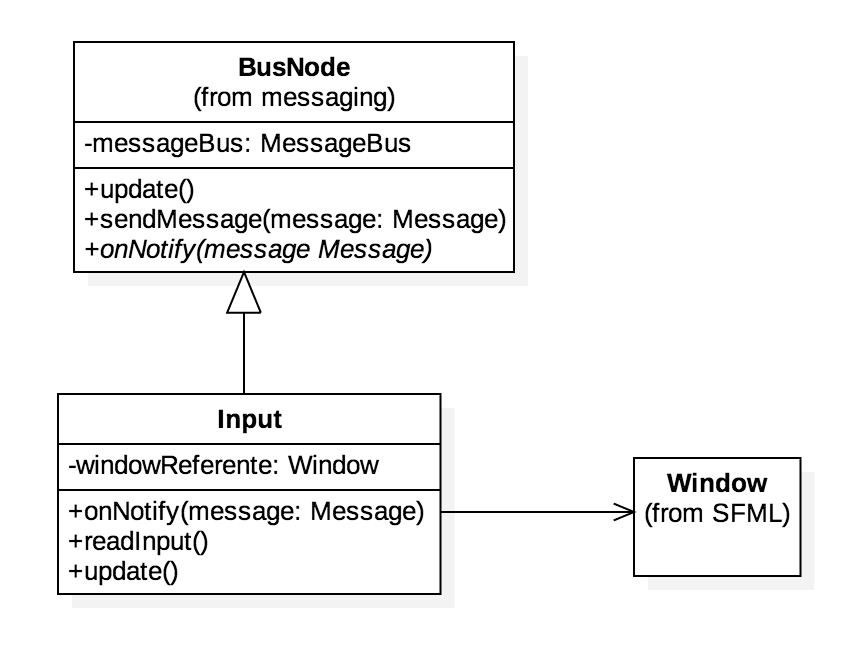
\includegraphics[width=12cm]{otros/UML/png/alld/png/input__diagramaDeClases_input_8.png}}
	\caption{Diagrama de clases del subsistema de entrada}
	\label{class:input}
\end{figure}

La figura \ref{class:input} muestra las clases referentes al subsistema de entrada. En dicho diagrama se puede observar como su definición es muy sencilla ya que solamente tendrá que iterar sobre todos los eventos de entrada que ocurren y enviarlos al bus de mensajes.

\bigskip

La clase principal \textit{Input} tendrá una asociación con la clase \textit{Window} de \textit{SFML} ya que es dicha clase la que genera todos los eventos. Internamente, dentro de la función \textit{update}, se irán recogiendo los eventos y enviándolos al bus de mensajes con el mensaje adecuado.


\subsubsection*{Subsistema de físicas}

\begin{figure}
	\centerline{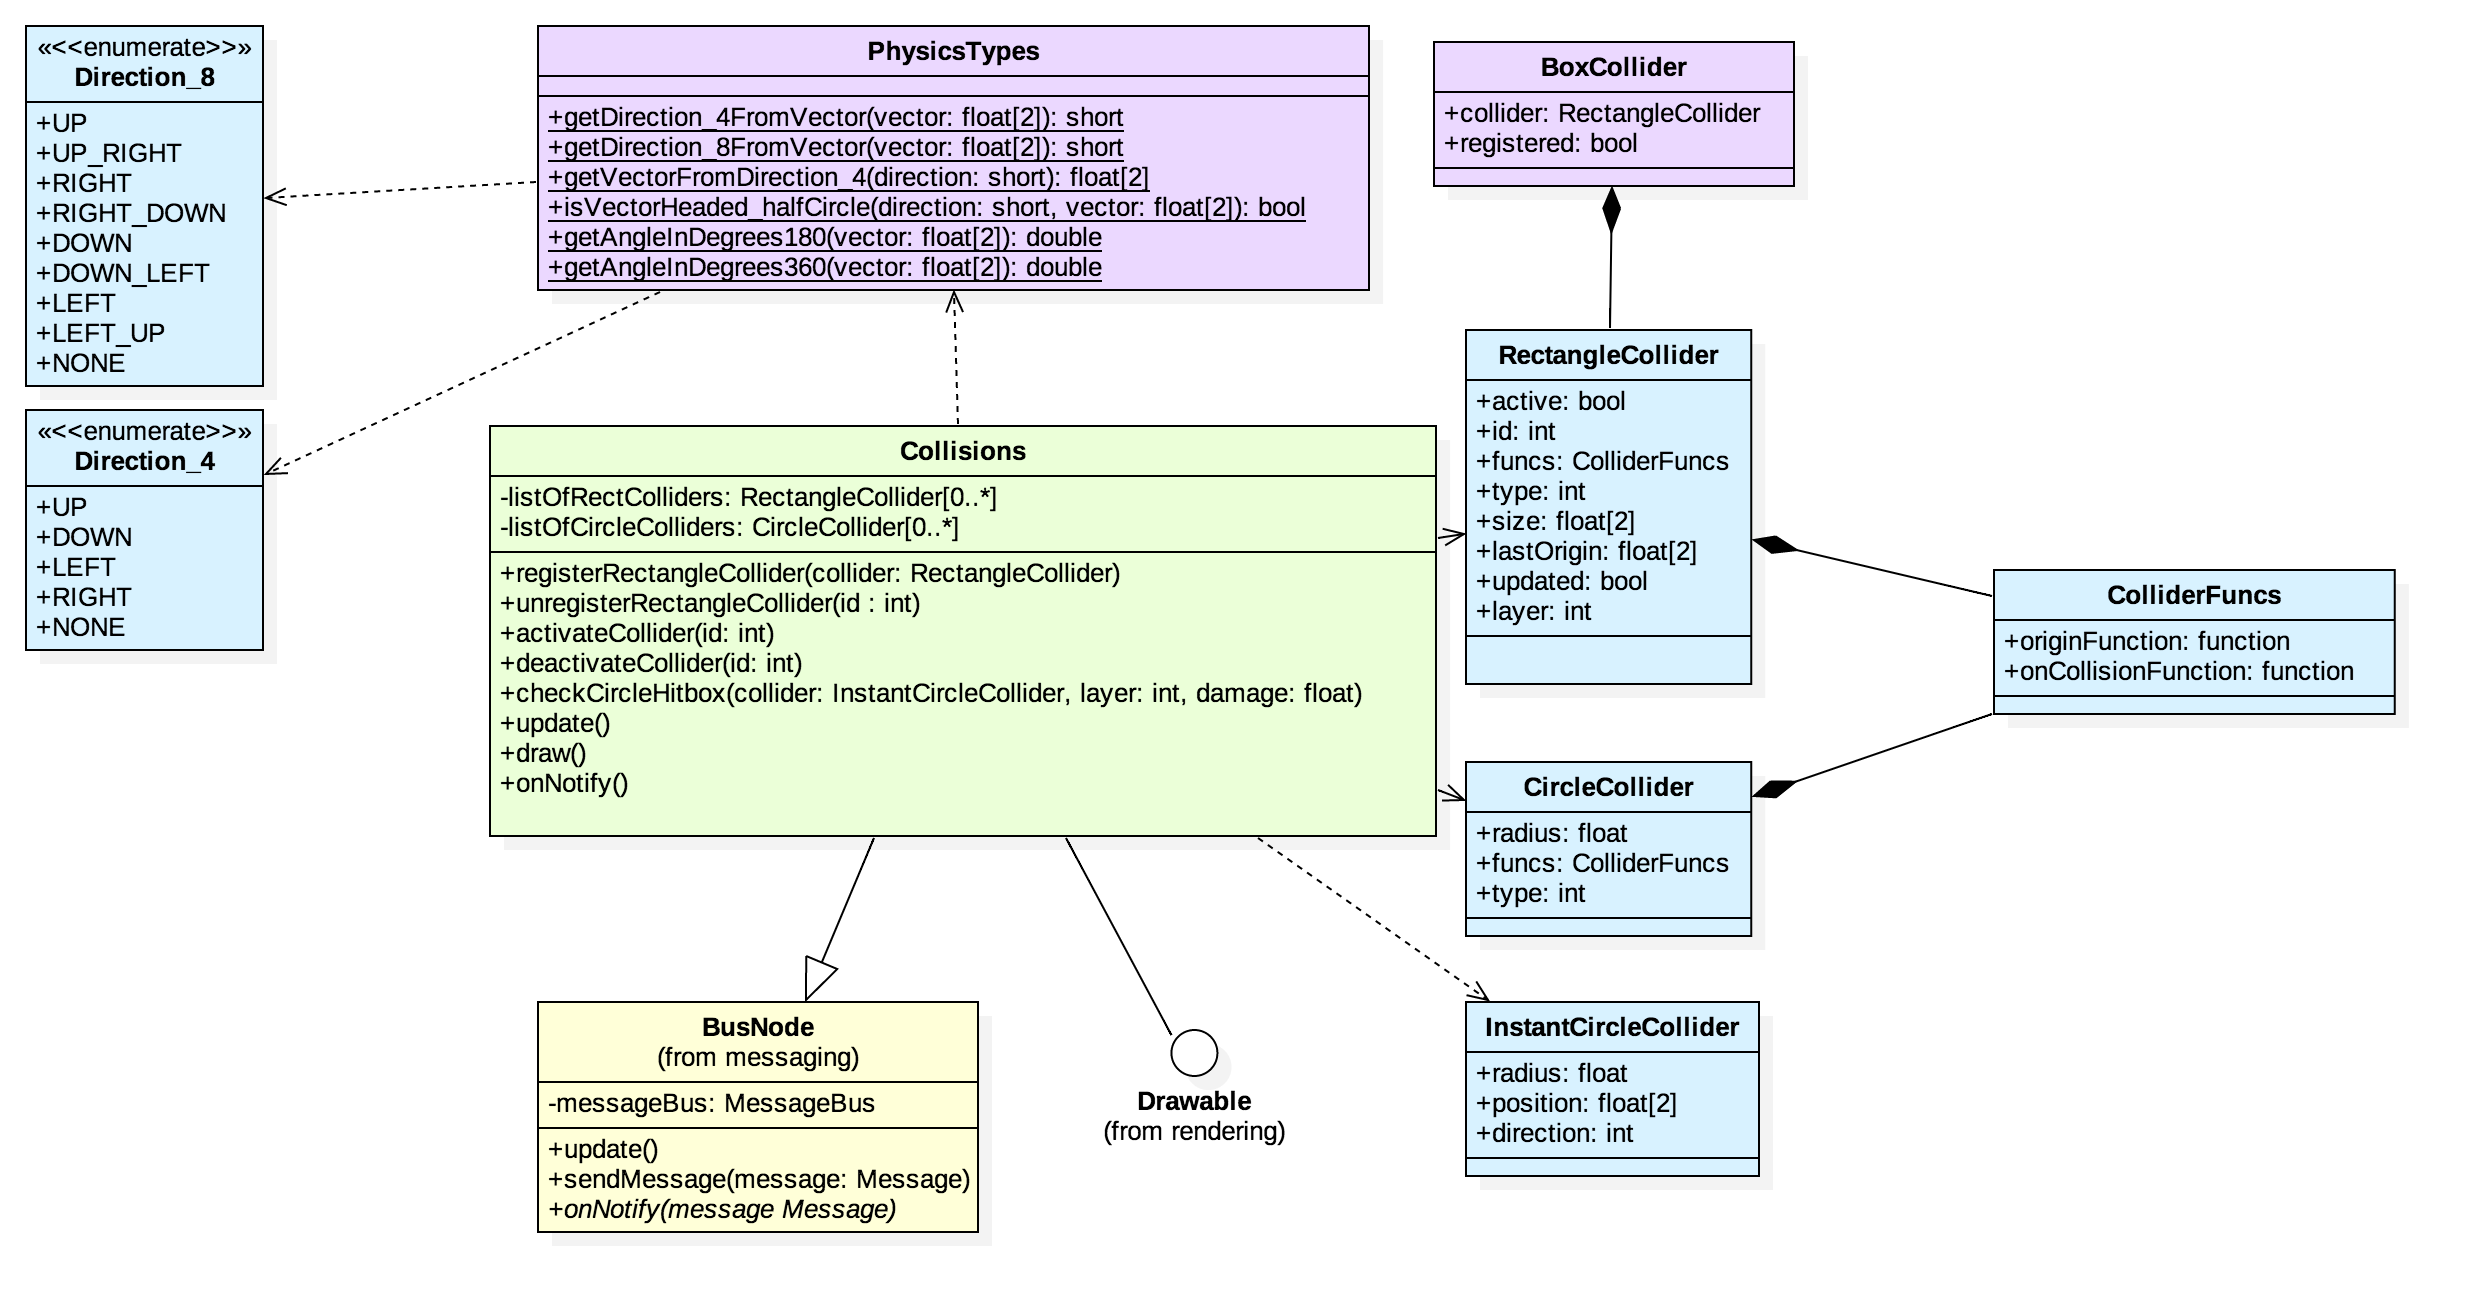
\includegraphics[width=18cm]{otros/UML/png/alld/png/physics__diagramaDeClases_physics_2.png}}
	\caption{Diagrama de clases del subsistema de físicas}
	\label{class:collisions}
\end{figure}

El subsistema de físicas está representado en el diagrama de clases de la figura \ref{class:collisions}. En el mismo destaca la clase \textit{\textbf{Collisions}} que se encarga de guardar los \textit{\textbf{RectangleColliders}} y \textbf{\textit{CircleColliders}} de la aplicación. Estos \textit{colliders} representan las diferentes figuras que pueden sufrir colisiones dentro de una escena y pueden tener forma de rectángulo o círculo. Ambos \textit{colliders} también contienen referencias a funciones capaces de proveer la posición actual del collider y que contienen la función a ejecutar si ocurre una colisión. Dichas funciones las contiene la estructura \textbf{\textit{ColliderFuncs}}.

\bigskip
\textbf{\textit{InstantCircleCollider}} es una estructura que permite comprobar instantáneamente si un circulo arbitrario colisiona con algún otro \textit{collider}. La inmediatez que esto permite es especialmente importante para comprobar si un ataque de un personaje ha acertado o no. Por otra parte, \textbf{\textit{BoxCollider}} es una clase que encapsula un \textit{RectangleCollider} para hacer transparente su creación y registro a otras clases de la aplicación.

\bigskip
Finalmente, \textbf{\textit{PhysicsTypes}} contendrá estructuras que representan direcciones en 4 u 8 sentidos (\textbf{\textit{Direction\_4}} y \textbf{\textit{Direction\_8}} respectivamente) y apostará funciones útiles para trabajar con ellos.


\subsubsection*{Subsistema de renderizado}

\begin{figure}
	\centerline{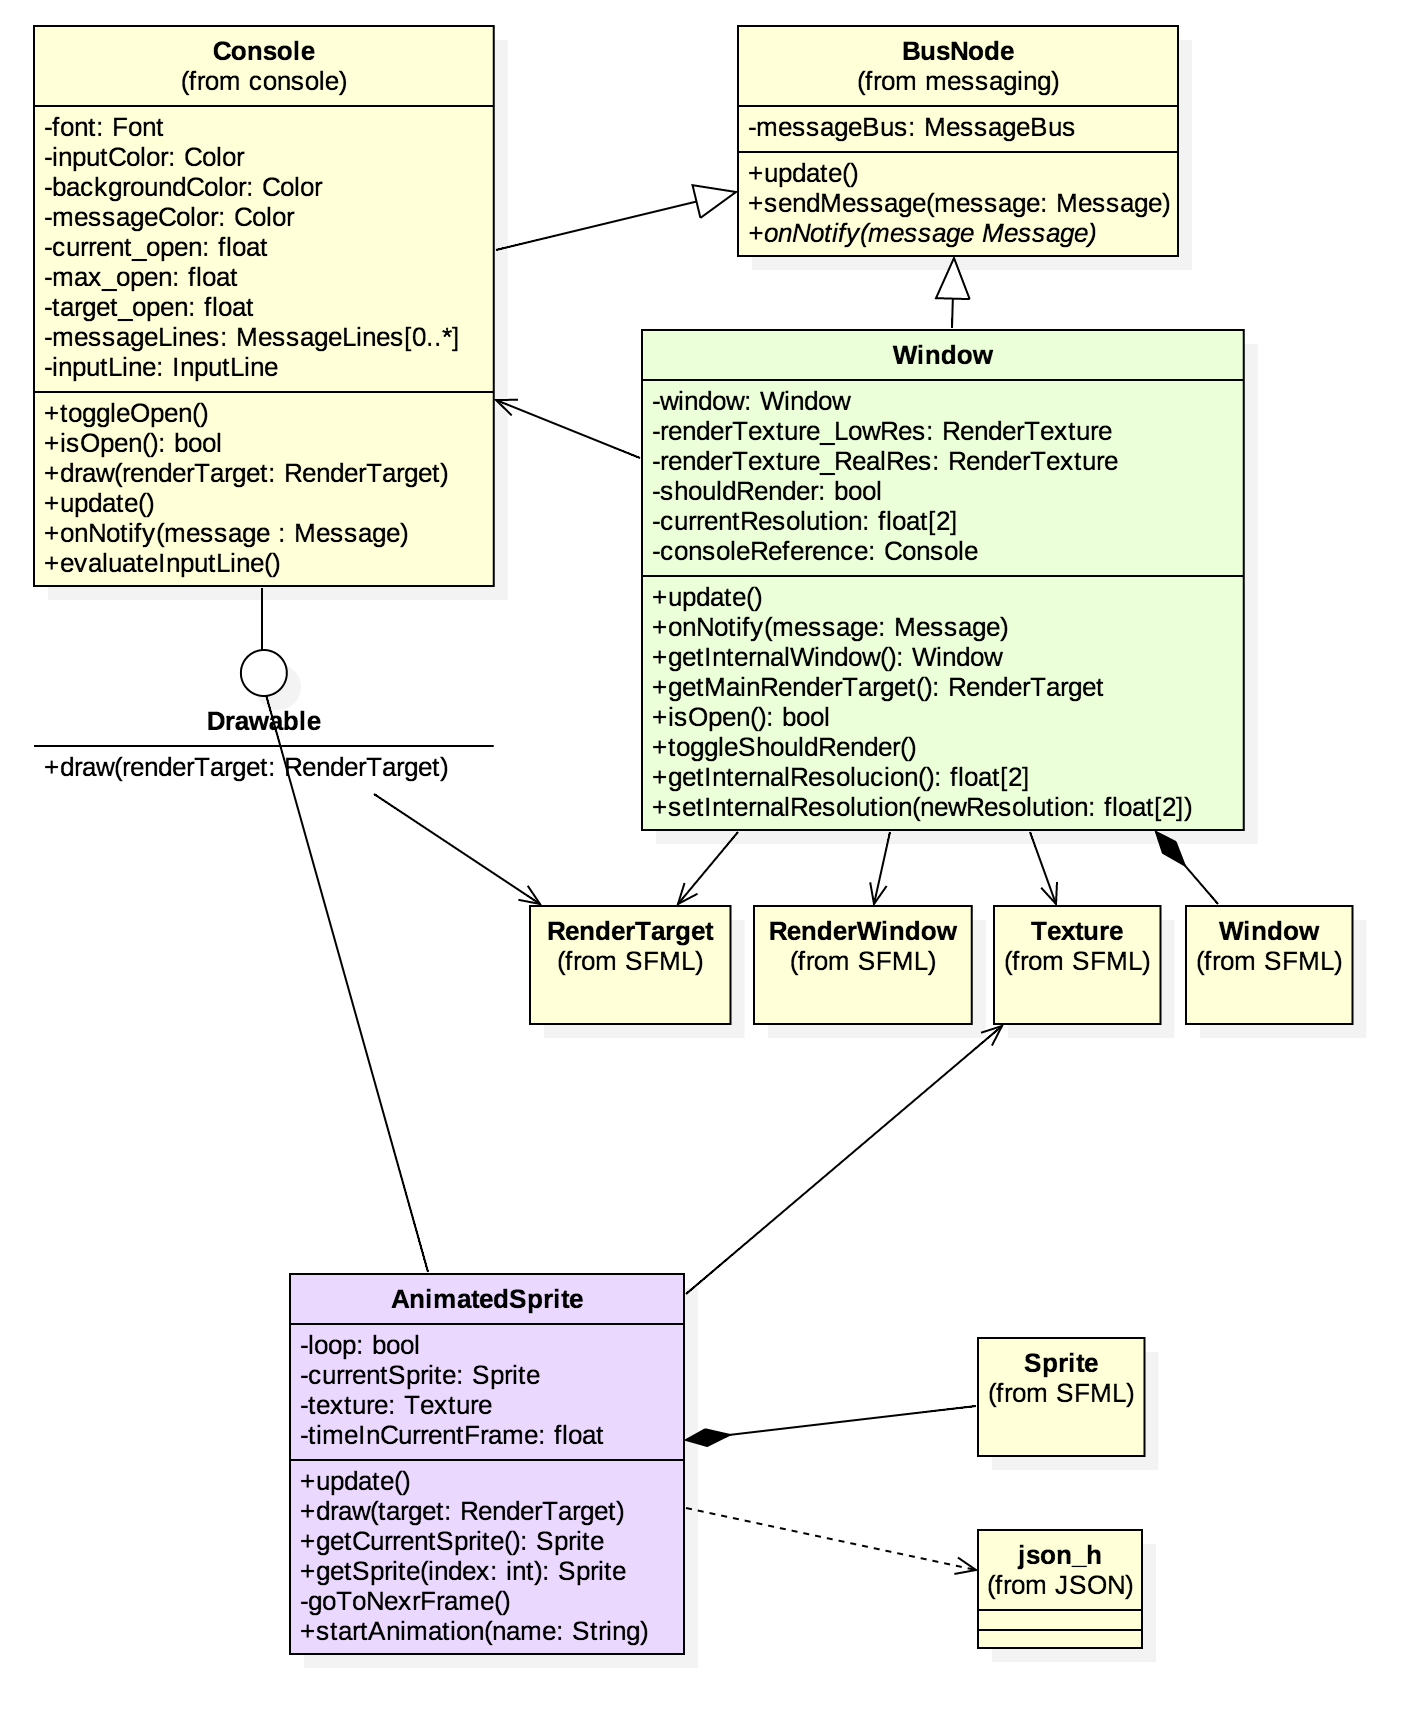
\includegraphics[width=15cm]{otros/UML/png/alld/png/rendering__diagramaDeClases_rendering_9.png}}
	\caption{Diagrama de clases del subsistema de renderizado}
	\label{class:rendering}
\end{figure}

El subsistema de renderizado, mostrado en la figura \ref{class:rendering}, contiene la clase principal \textbf{\textit{Window}} encargada de mostrar por pantalla la aplicación. Para ello aporta funcionalidades como:

\begin{itemize}
	\item Parar de mostrar o volver a mostrar la aplicación con \textit{toggleShouldRender}.
	\item Cambiar la resolución interna de la aplicación independientemente de la externa con \textit{setInternalResolution}.
	\item Comprobar si la ventana sigue abierta para terminar la aplicación.
\end{itemize}

Para dibujar por pantalla hará uso de una serie de atributos, muchos de ellos aportados por la librería \textit{SFML}:

\begin{itemize}
	\item \textbf{\textit{window}}: Objeto de la clase \textit{Window} de \textit{SFML} que representa la funcionalidad más básica de una ventana en el sistema operativo en el que se está ejecutando.
	\item \textbf{\textit{renderTextures}}: Dos objetos de la clase \textit{RenderTexture} de \textit{SFML} que representan texturas sobre las que se dibuja, una de ellas estará a baja resolución y se pintará el juego sobre ella para ahorrar recursos. Luego se escalará esa misma textura y se pintará por encima de la de alta resolución que es la que finalmente se muestra por pantalla.
	\item \textbf{\textit{shouldRender}}: Booleano que define si se muestra o no algo por pantalla.
	\item \textbf{\textit{currentResolution}}: Que guarda la resolución real de la ventana.
	\item \textbf{\textit{consoleReferente}}: Referencia a la consola que permite pintarla siempre que sea necesario, independientemente de que exista una escena o de que el juego se encuentre detenido.
\end{itemize}

\bigskip

Además, la clase \textbf{\textit{AnimatedSprite}} guarda una textura en formato png que contiene todos los dibujos de un personaje en las diferentes posturas que forma una animación, lo que se conoce como \textit{spritesheet}. Para mostrar el dibujo correcto se lee previamente un archivo en formato JSON con ayuda de \textbf{\textit{json.h}} que contiene las animaciones y donde están localizadas cada imagen individual dentro de la textura general.

\bigskip

Esta clase ofrece una forma general de guardar y mostrar movimiento de cara a \textit{gameobjects} con animaciones.

\subsubsection*{Subsistema de renderizado}

\begin{figure}
	\centerline{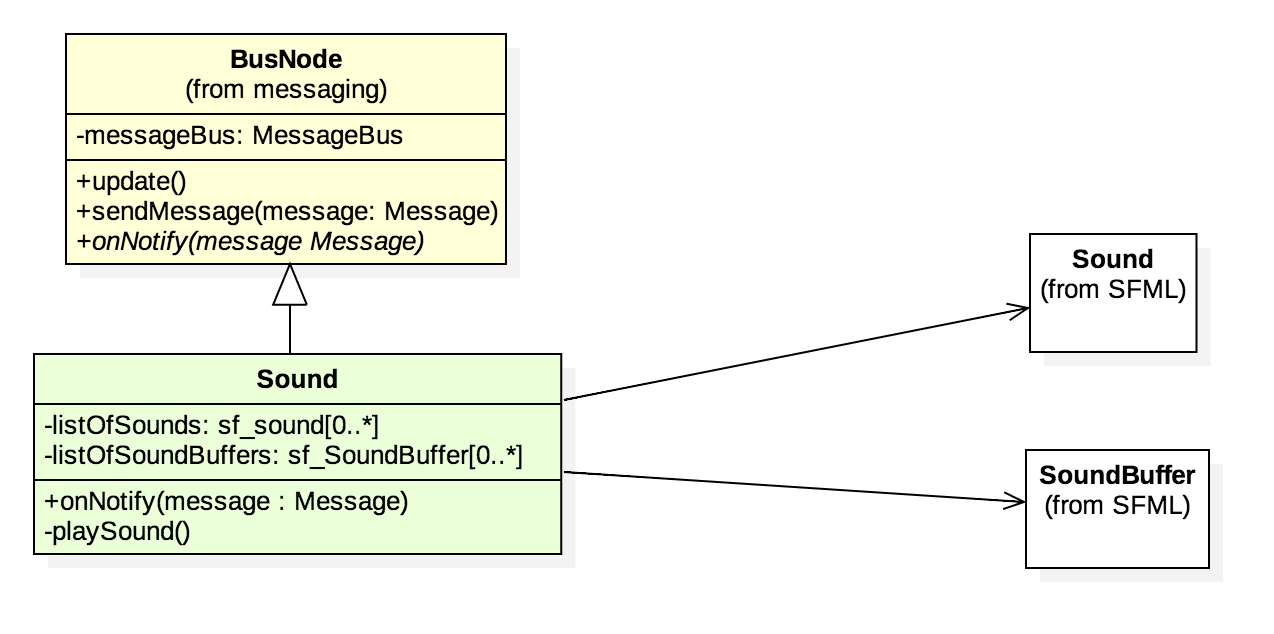
\includegraphics[width=15cm]{otros/UML/png/alld/png/sound__diagramaDeClases_sound_1.png}}
	\caption{Diagrama de clases del subsistema de sonido}
	\label{class:sound}
\end{figure}

Finalmente, se puede observar el diagrama del subsistema de sonido en la figura \ref{class:sound}. El mismo es muy sencillo, ya que los sonidos (representados por la clase \textbf{\textit{Sound}}) unicamente son cargados al inicializar el subsistema, junto con los \textit{buffers} (representados por la clase \textbf{\textit{SoundBuffer}}) necesarios para su reproducción que guardan datos referentes a cada \textit{tick} dentro del archivo de sonido.

\bigskip

Internamente, se utilizarán dos listas con dichos sonidos y \textit{buffers} que serán accedidos cuando se utilice la función \textbf{\textit{playSound}} para comenzar la reproducción de un sonido. La única forma de que se ejecute \textit{playSound} es que llegue un mensaje concreto para cada sonido desde el bus de mensajes.

\subsection{Otros útiles}

\subsubsection*{Paquete de recursos}

\begin{figure}
	\centerline{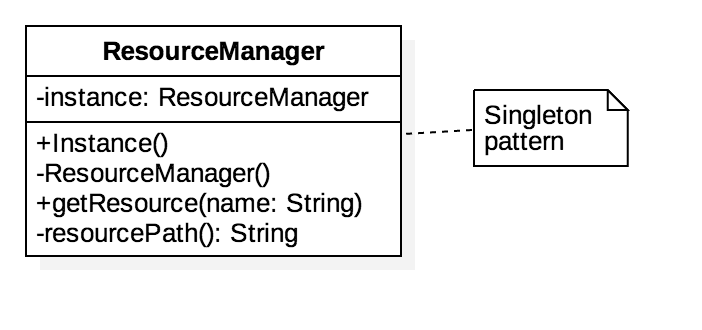
\includegraphics[width=8cm]{otros/UML/png/alld/png/resources__diagramaDeClases_resources_0.png}}
	\caption{Diagrama de clases del paquete de recursos}
	\label{class:resources}
\end{figure}

La clase \textbf{\textit{ResourceManager}} mostrada en la figura \ref{class:resources} es la encargada de hacer que todos los recursos que necesita el juego estén disponibles en tiempo de ejecución. Para lograr esto se ha implementado un \textit{Singleton} que contiene partes en el lenguaje \textit{Objective-C}. Esto permite trabajar directamente con el sistema operativo de Apple y acceder a recursos embebidos dentro del ejecutable \textit{.app} de la aplicación.

\bigskip

La funcionalidad básica de \textbf{\textit{getResource}} buscará y devolverá un recurso determinado con el nombre dado. Además, la función de \textbf{\textit{resourcePath()}} devolverá siempre una ruta válida hasta los recursos de la aplicación (fuentes, sonidos, imágenes, etc.).

\subsubsection*{Paquete de útiles}

\begin{figure}
	\centerline{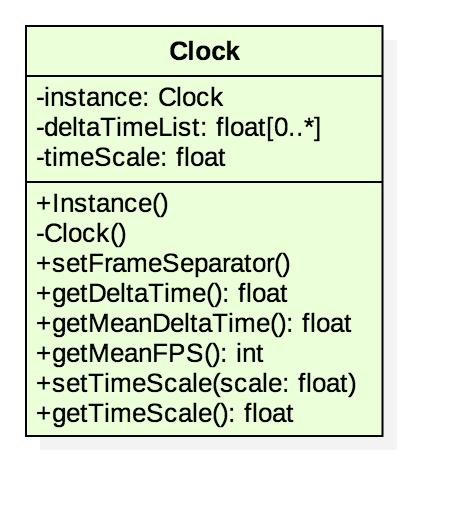
\includegraphics[width=5cm]{otros/UML/png/alld/png/utils__diagramaDeClases_utils_10.png}}
	\caption{Diagrama de clases del paquete de útiles}
	\label{class:utils}
\end{figure}

Por último se muestra el paquete de utilidades comunes en la figura \ref{class:utils}. El mismo solo contiene la clase \textbf{\textit{Clock}}, un \textit{Singleton} que representa el reloj interno de la aplicación. El mismo es capaz de determinar el tiempo que ha transcurrido entre fotogramas para calcular de forma precisa el movimiento y físicas del videojuego.

\bigskip

Además proporciona la posibilidad de escalar su velocidad mediante \textbf{\textit{setTimeScale}} permitiendo así las simulaciones aceleradas referenciadas en el RNF-2.

\bigskip

Este paquete podría contener cualquier funcionalidad común y útil para varios subsistemas pero ya que las mismas están convenientemente encapsuladas en dicho subsistemas no ha sido necesario agrupar muchas funcionalidades en el presente paquete.

\subsection{Escenas}

\subsubsection*{Escena del menú}

\begin{figure}
	\centerline{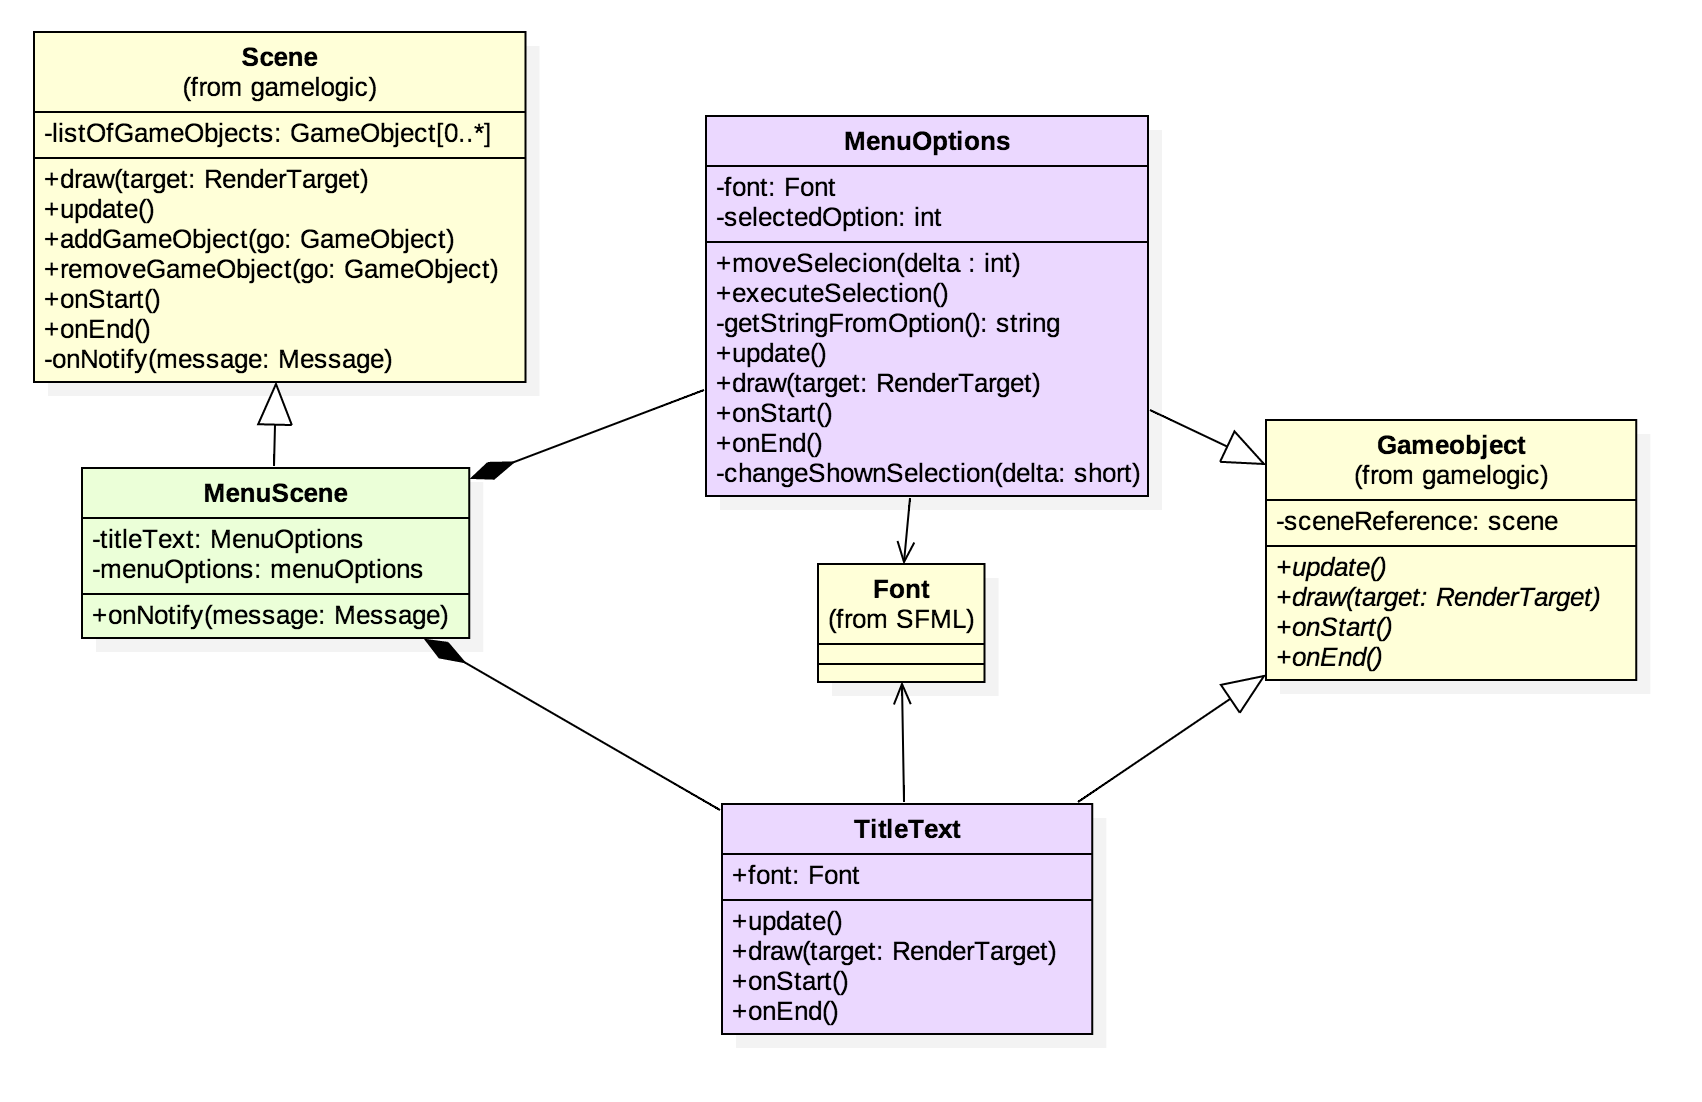
\includegraphics[width=15cm]{otros/UML/png/alld/png/gamelogic__menu__diagramaDeClases_scene_menu_6.png}}
	\caption{Diagrama de clases de la escena del menú}
	\label{class:menu}
\end{figure}

La escena del menú, mostrada en la figura \ref{class:menu}, es la escena más sencilla de la aplicación. Contiene los siguientes \textit{gameobjects}:

\begin{itemize}
	\item \textbf{\textit{TitleText}}: Simplemente usado para mostrar el título del juego.
	\item \textbf{\textit{MenuOptions}}: Contiene las diferentes opciones del menú, se encarga de guardar la que está seleccionada, cambiar esta selección y ejecutar la seleccionada cuando se requiere.
\end{itemize}

\subsubsection*{Escena de juego}

\begin{figure}
	\caption{Diagrama de clases de la escena de juego}
	\hspace*{-0.1cm}  
	\centerline{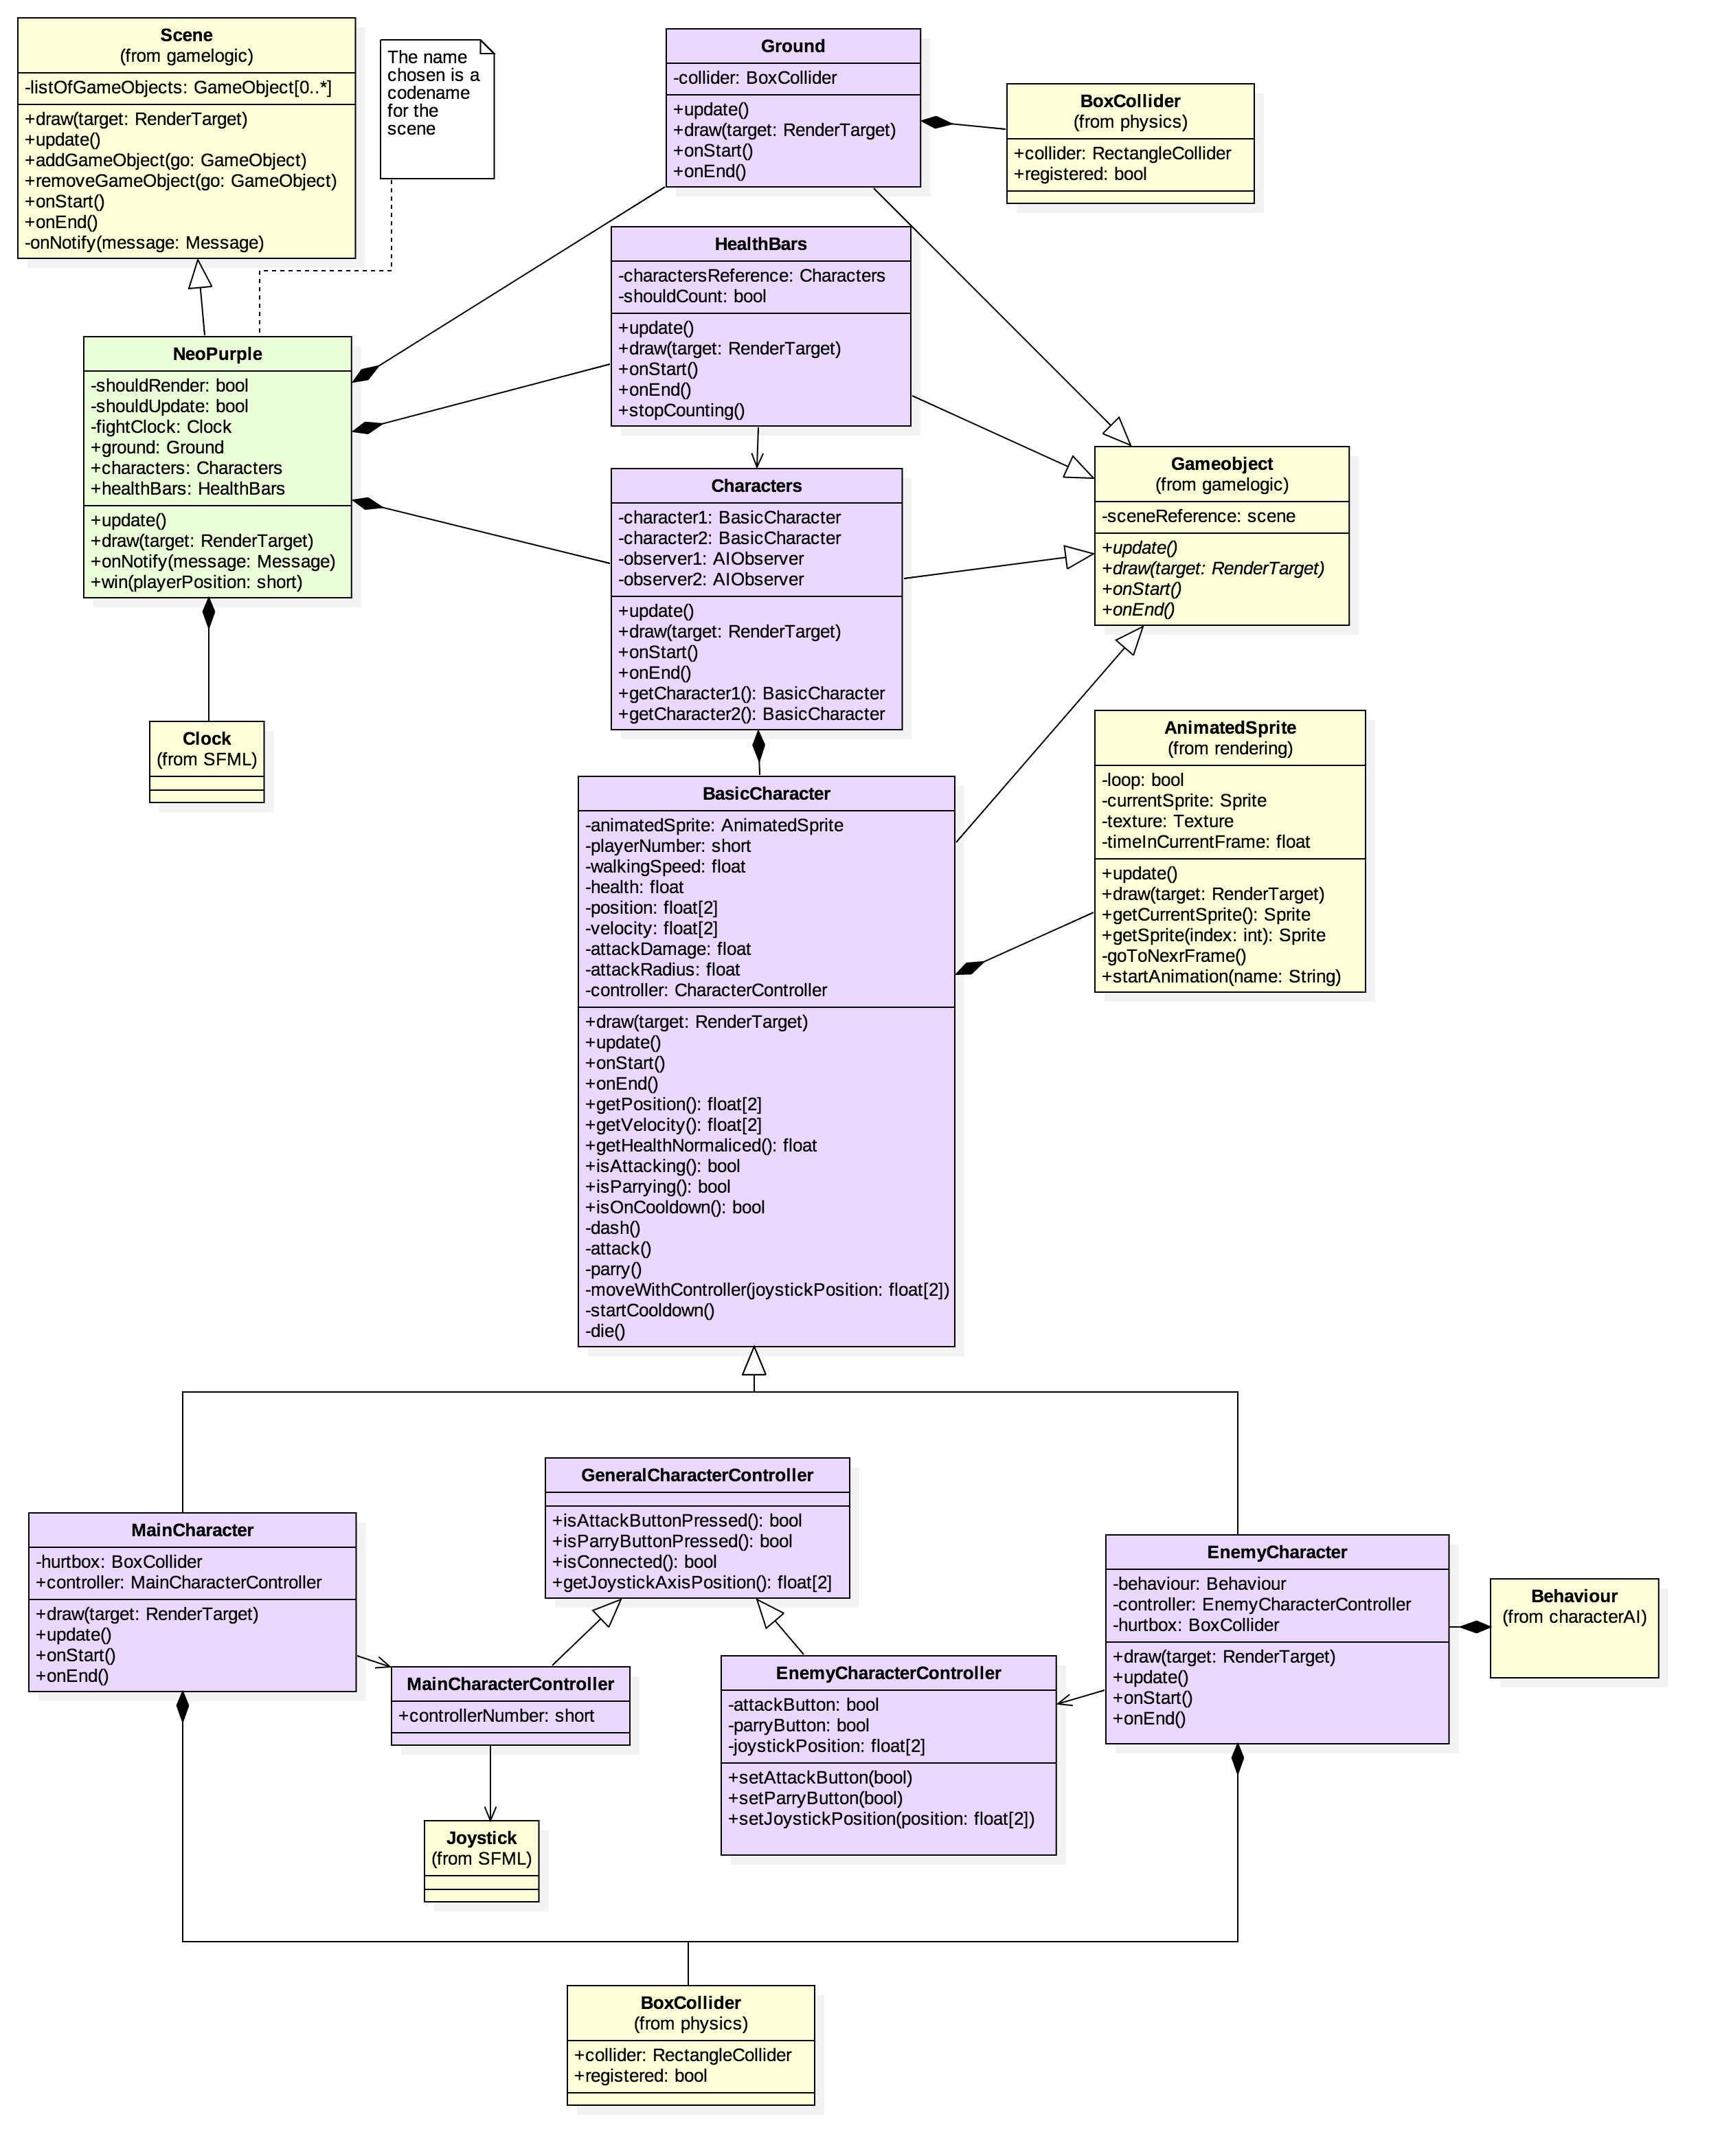
\includegraphics[width=20cm]{otros/UML/png/alld/png/gamelogic__gameplay__diagramaDeClases_scene_gameplay_4.png}}
	\label{class:gameplay}
\end{figure}

Esta escena (figura \ref{class:gameplay}) es la dedicada a jugar realmente al videojuego, la misma contiene el combate entre los dos personajes. La clase dedicada a la escena es \textbf{\textit{NeoPurple}}\footnote{nombre en clave escogido por la apariencia del suelo de la escena para identificarla fácilmente en caso de que se requirieran más escenas con \textit{gameplay}} y se encarga de contener a todos los \textit{gameobjects} necesarios y a gestionar la victoria de uno de los personajes con la función \textbf{\textit{win}}. Los \textit{gameobjects} contenidos en la escena son:

\begin{itemize}
	\item \textbf{\textit{Ground}}: Encargado de representar el suelo de la escena, es el encargado tanto de pintar el suelo como de proporcionar al sistema de colisiones un \textit{collider} que impida que los personajes se salgan de la escena mediante el uso de ese \textit{BoxCollider}.
	\item \textbf{\textit{HealthBars}}: Muestra la vida de los dos personajes y el tiempo de pelea restante, tiene una referencia a \textit{Characters} para obtener información sobre la vida de ambos.
	\item \textbf{\textit{Characters}}: Contiene e identifica a los dos personajes en la escena, no solo facilita acceder a ellos por parte de las clases que lo requieran sino que ayuda a reconocer cual es el personaje 1 y 2 y saber por que están siendo controlados (jugador, agente, sistema de reglas, etc).
	\item \textbf{\textit{BasicCharacter}}: Clase genérica que representa un personaje, contiene todas las funciones de movimiento y acciones que el mismo puede realizar (\textit{attack}, \textit{parry} y \textit{moveWithController}). Además contiene todos los atributos que definen sus características como la vida (\textit{health}), rango (\textit{attackRadius}), velocidad (\textit{velocity}), posición (\textit{position}), daño (\textit{attackDamage}), etc. 
	\item \textbf{\textit{MainCharacter}}: Clase que representa a un personaje controlado por el jugador, hace uso de la clase \textbf{\textit{MainController}} que representa un mando real conectado el equipo.
	\item \textbf{\textit{EnemyCharacter}}: Clase que representa a un personaje controlado por la aplicación, contiene un mando virtual representado por \textbf{\textit{EnemyController}} que será modificado por el comportamiento o \textbf{\textit{Behaviour}} del que se habla en el siguiente apartado.
\end{itemize}

\bigskip

Ambos personajes cuentan con una instancia de \textit{BoxCollider} que representa el \textit{collider} usado para recibir daño.

\subsubsection*{Comportamiento del agente}

El diagrama contenido en la figura \ref{class:agent} es uno de los más complejos de la aplicación. De hecho, debería de estar en la figura \ref{class:gameplay} ya que forma parte del \textit{gameplay} pero dada su importancia y complejidad se ha decidido dedicar esta sección al mismo en aras de evitar diagramas enormes imposibles de ver en un documento de este formato y de entender a primera vista. Para explicar sus partes se dedicará una parte deparada a cada uno de los conjuntos de componentes.

\bigskip

Comenzando por la parte izquierda se ven las clases que representan el estado de la pelea a ojos del agente. La versión continua del estado está contenida en \textbf{\textit{FightState}} que contendrá el estado de ambos personajes representado por la clase \textbf{\textit{CharacterState}}.

\bigskip
La clase \textbf{\textit{Observer}} es el componente encargado de representar los \textit{ojos} del agente en el sentido de ver la situación de los personajes y representarla de un modo adecuado. Por lo tanto, será este el encargado de discretizar el estado continuo para obtener un objeto de la clase \textbf{\textit{FightState\_Discrete}}. Esta clase contiene el estado propio del personaje y del enemigo en \textbf{\textit{MyCharacterState\_Discrete}} y \textbf{\textit{OtherCharacterState\_Discrete}} respectivamente. Es importante mencionar que solo el estado propio contiene datos de posición ya que la misma se define de forma relativa al enemigo en la clase \textbf{\textit{Position\_Discrete}} de forma que se evita duplicar información.

\bigskip

Pasando ahora a la jerarquía de clases de \textbf{\textit{Behaviour}} se ve como la clase principal es la encargada de representar la estrategia genérica del patrón \textit{Strategy}\ref{pat:strategy} ya que el enemigo siempre tendrá una pero podrá cambiar entre ellas en diferentes ejecuciones. Esta clase \textit{Behaviour} tiene acceso a la clase \textbf{\textit{Actions}} que encapsula las acciones posibles a realizar y las ejecuta con \textbf{\textit{execute}} sobre la referencia al \textit{controller} que contiene. Algo importante es el hecho de que \textit{Behaviour} contiene un \textit{thread} independiente que correrá todos los cálculos referentes a la inteligencia artificial del juego, separando de forma efectiva la complejidad del juego con la del agente y favoreciendo el rendimiento.

\bigskip

\textbf{\textit{RuleBasedBehaviour}} es la implementación base sobre la que probar al agente. La misma especifica las acciones que llevará a cabo el enemigo en cada situación y se ha realizado gracias al \textbf{conocimiento experto} del desarrollador pues el mismo tiene experiencia jugando al juego. Solo necesita acceso al estado actual de la pelea (\textbf{\textit{currentState}}) para elegir la acción programada.

\bigskip

\textbf{\textit{ReinforcementBehaviour}} es la clase que contiene el comportamiento que el agente ha aprendido. El mismo se ha generado a partir de la exploración de estados posibles y de la mejora en la función de \textit{fitness} que ha supuesto cada acción. Para calcular este \textit{fitness} se hace uso de la función \textbf{\textit{calculateFitness}} en \textit{Observer}.

\bigskip

Para representar la información referente a los estados visitados se guarda el estado actual (\textbf{\textit{currentState}}) y el último (\textbf{\textit{lastState}}), además de la ultima acción escogida (\textbf{\textit{lastAction}}). Con estos datos, al principio de cada iteración del \textbf{\textit{update}}, se guardará en el \textit{StateActionContainer} la mejora en el \textit{fitness} asociada a una acción para un determinado estado. Luego se obtendrá el estado actual y si este no ha sido visitado se escogerá una acción aleatoria, si por el contrario este ha sido visitado, se escogerá entre las posibles acciones teniendo en cuenta el \textit{fitness} esperado para cada una, habiendo una posibilidad de que aleatoriamente se escoja una acción con poco \textit{fitness} para solucionar el conocido problema de exploración contra explotación\footnote{problema común en entornos de inteligencia artificial en el cual un agente debe balancear escoger siempre la opción que parece la mejor en este momento con explorar las otras posibles opciones en busca de otra que pueda ser superior.} en inteligencia artificial.

\bigskip

Por último, \textbf{\textit{StateActionContainer}} será un \textit{Singleton} encargado de representar el conocimiento sobre los estados. Las estructuras que representan este conocimiento son \textbf{\textit{StateActionSituation}} y \textbf{\textit{ActionSituation}} que contienen la información para un estado y para cada acción dentro del estado respectivamente. Además, \textit{StateActionContainer} es capaz de leer y guardar este conocimiento desde un archivo dentro del ejecutable para mantenerlo entre diferentes ejecuciones. Se podría usar la opción de \textbf{\textit{resetKnowledge}} si se quisiera que el agente olvidara todo lo aprendido hasta el momento.


\clearpage
\begin{landscape}
\begin{figure}
	\begin{adjustwidth}{-3cm}{}
		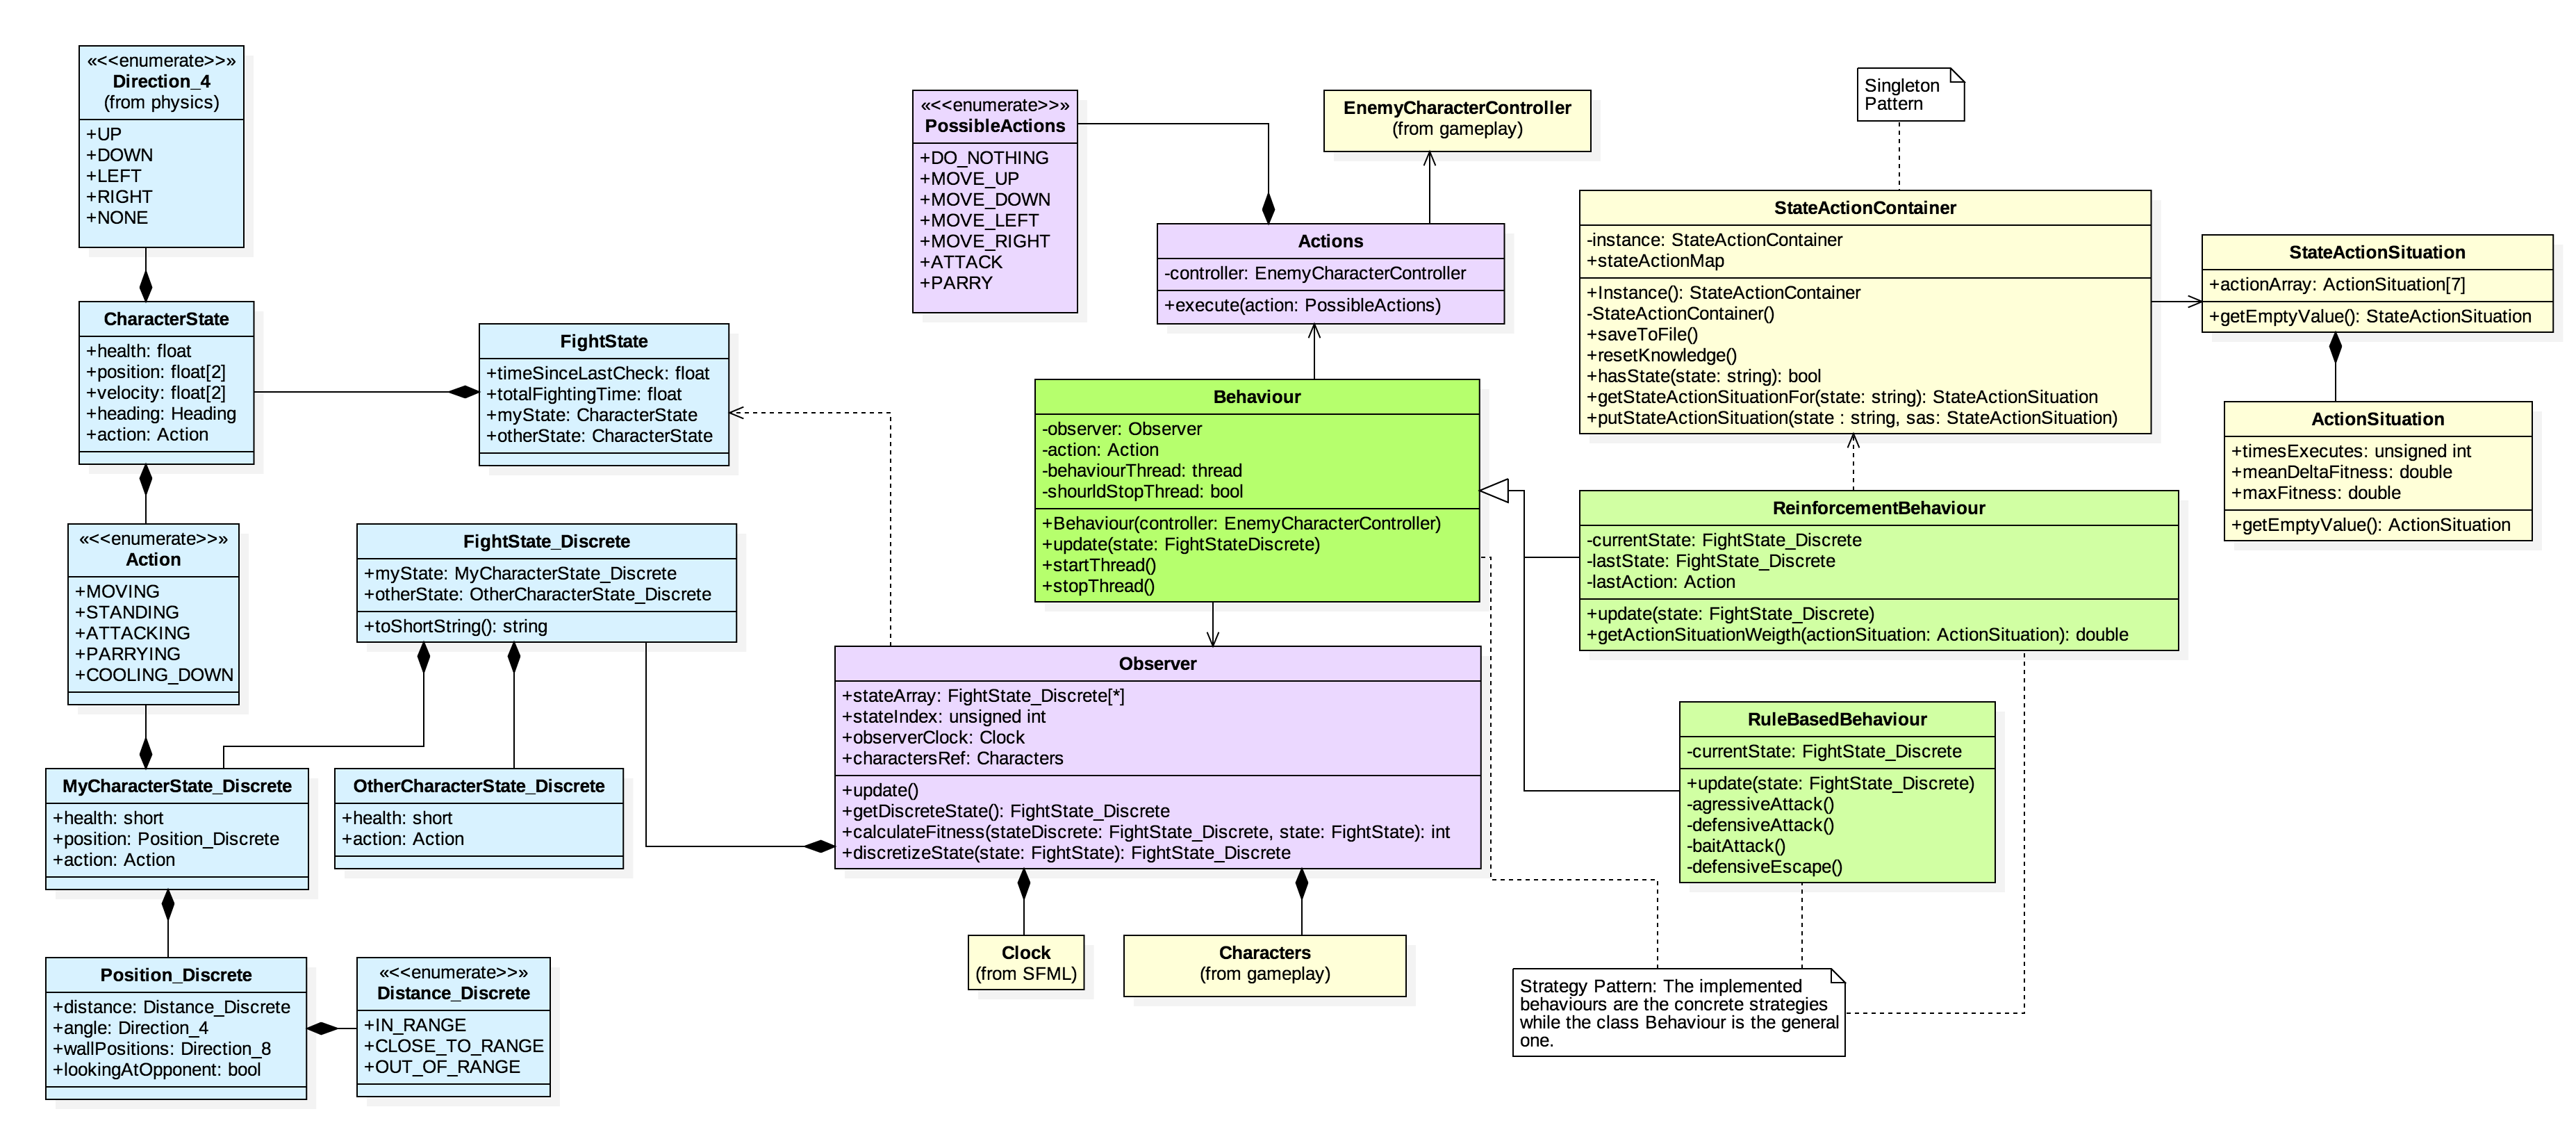
\includegraphics[width=24cm]{otros/UML/png/alld/png/gamelogic__gameplay__characterAI__diagramaDeClases_IA_5.png}
		\caption{Diagrama de clases del comportamiento del agente}
		\label{class:agent}
	\end{adjustwidth}
\end{figure}
\end{landscape}
\clearpage



\section{Diagramas de secuencia}

Esta sección estará dedicada a explicar la secuencia de operaciones que se realiza en casos comunes e importantes de partes de la aplicación. Se ha optado por mostrar partes clave de la aplicación en lugar de dedicar un diagrama de secuencia a cada caso de uso ya que si se hiciera de este modo se repetiría mucha información entre los mismos, además de dar lugar a diagramas de secuencia de tamaños excesivos. Otra nota importante es que no se suelen utilizar diagramas de secuencia en este tipo de arquitecturas y en especial en videojuegos ya que su naturaleza lleva a realizar acciones durante muchas diferentes del \textit{gameloop}\footnote{bucle principal de un videojuego en el que se actualizan todas sus partes, se puede ver un ejemplo en la figura \ref{sec:general}} haciendo que representar un caso de uso diera lugar a diagramas de secuencia con decenas de instancias y cientos de mensajes entre ellas.

\bigskip

En los siguientes párrafos se mostrarán diagramas de secuencia relevantes de la aplicación y se relacionarán con los casos de uso en los que son importantes. Se empieza por los diagramas asociados a la aplicación en general para luego seguir con los diagramas específicos relacionados con las escenas y el agente.

\subsection{Aplicación general}

\subsubsection*{Aplicación global}

\begin{figure}
	\centerline{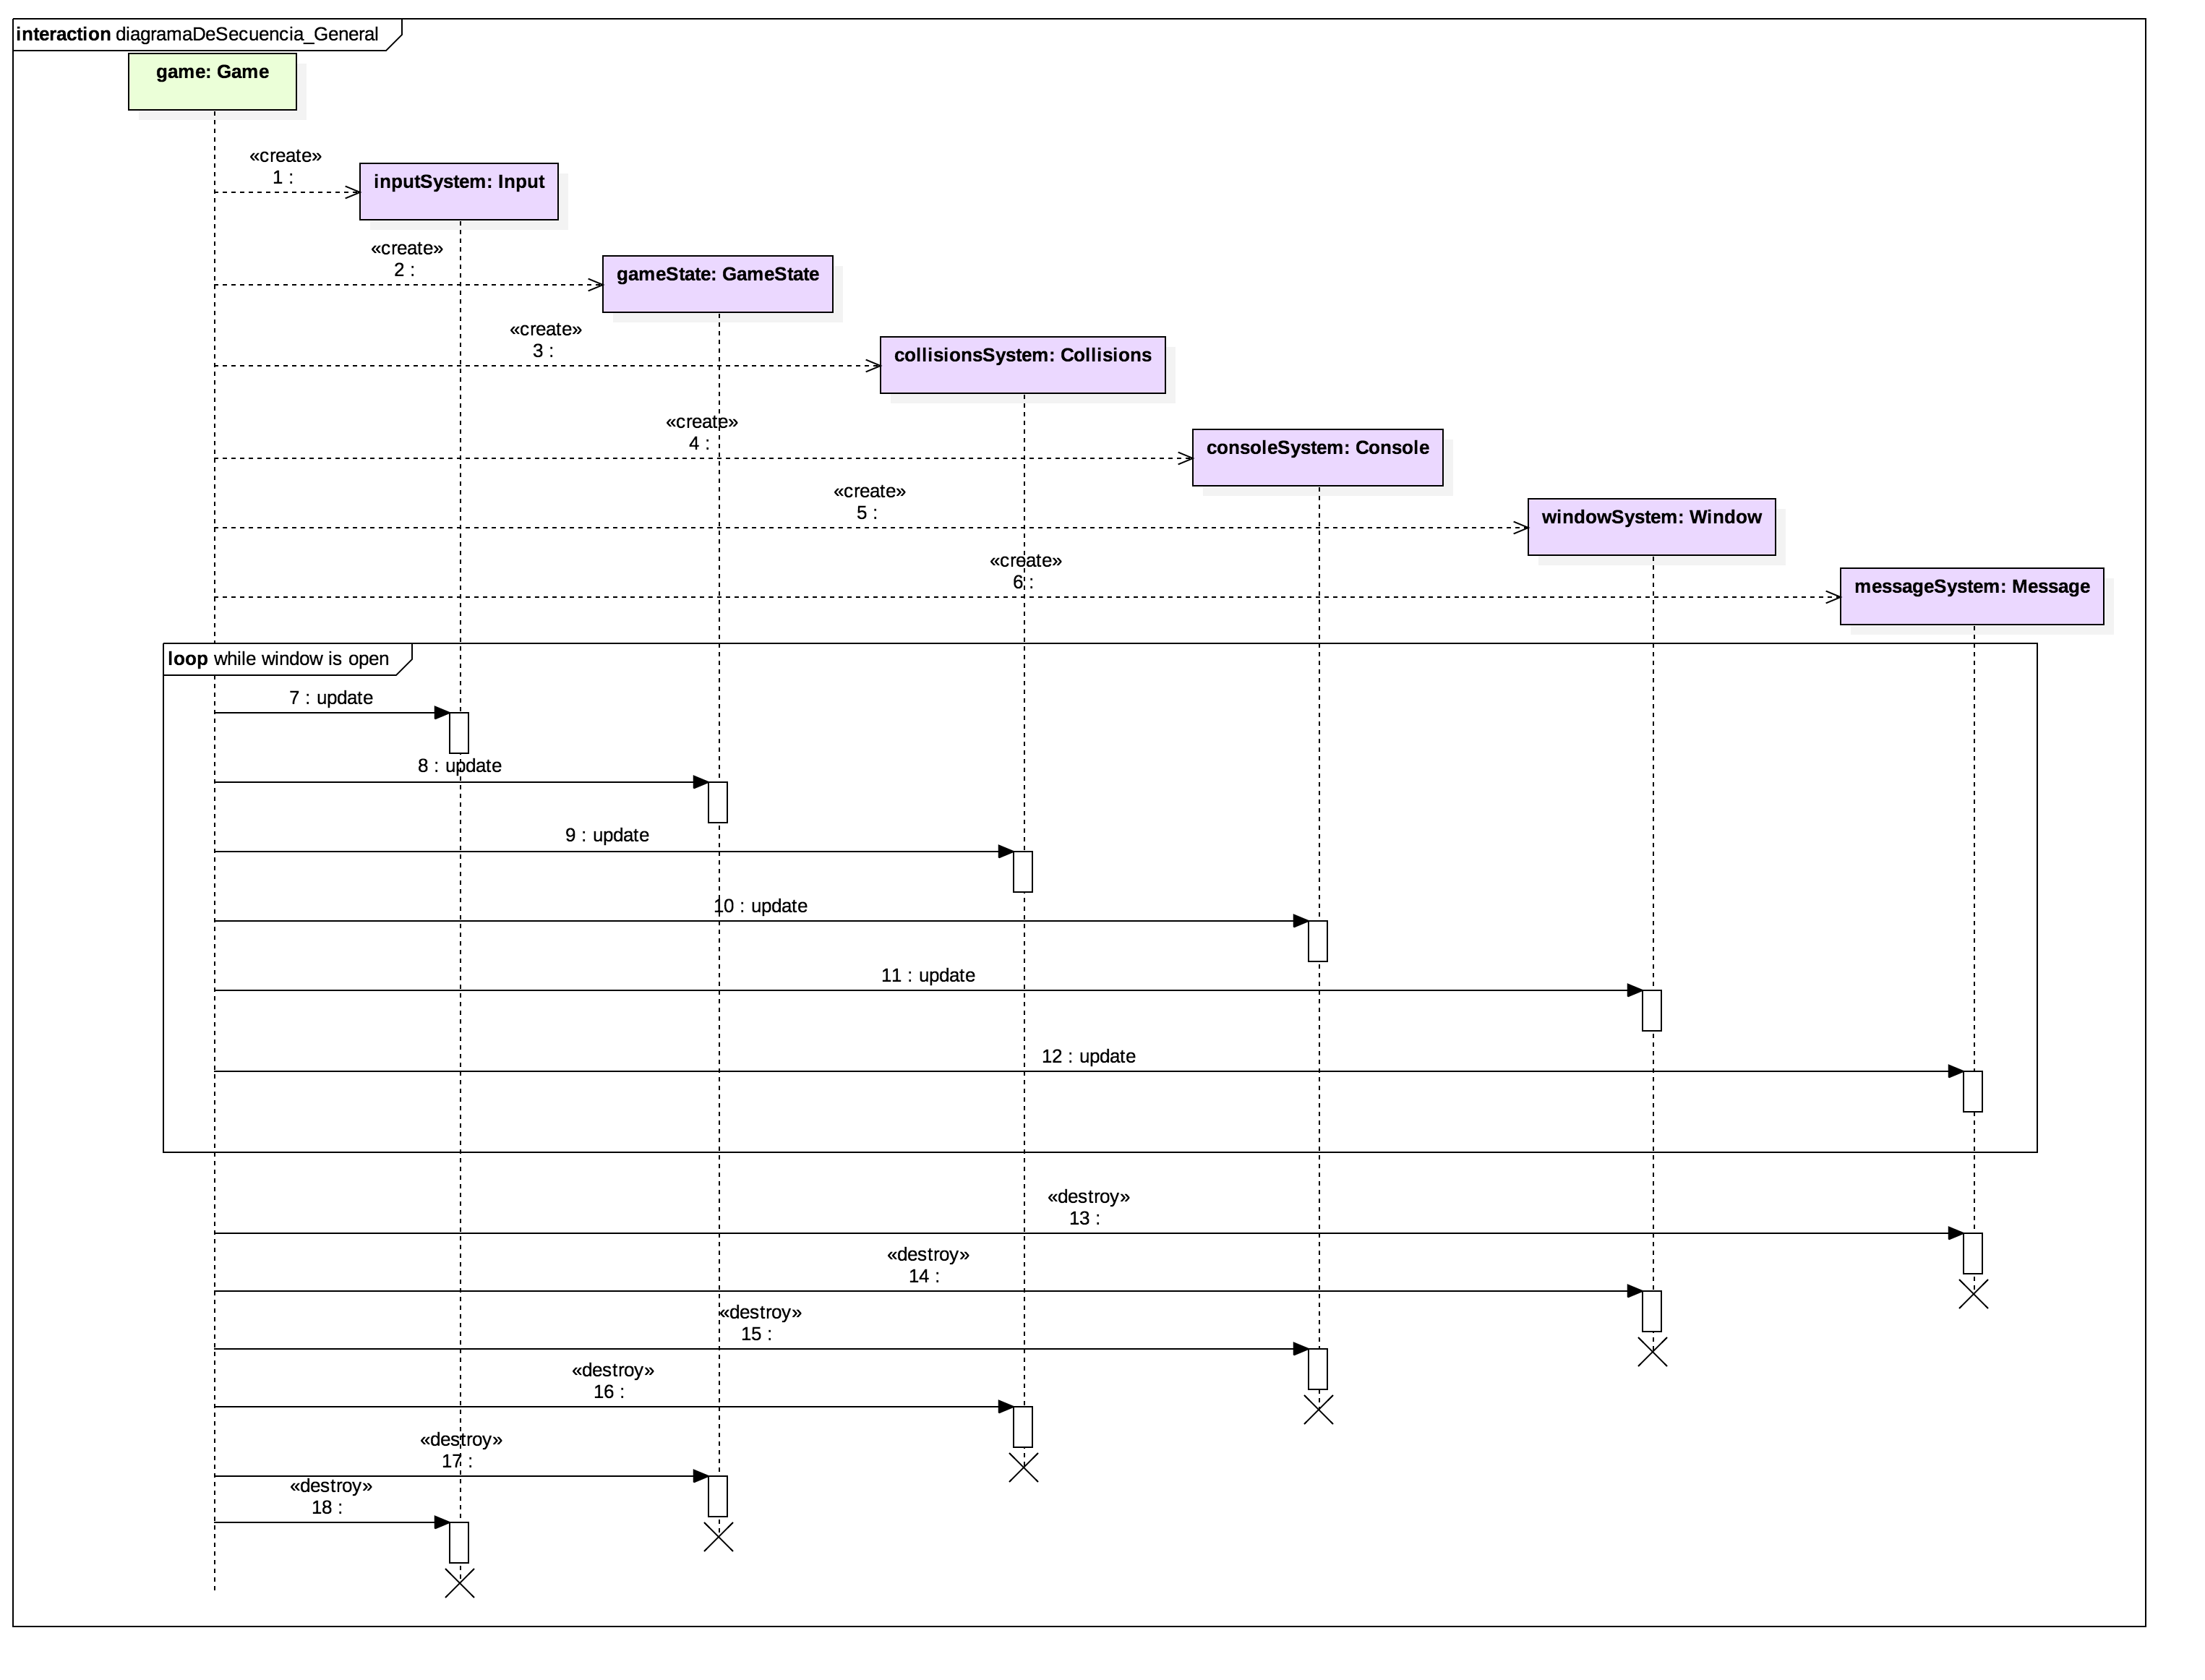
\includegraphics[width=19cm]{otros/UML/png/alld/png/CasosDeUso__General__Collaboration1__Interaction1__diagramaDeSecuencia_General_15.png}}
	\caption{Diagrama de secuencia general de la aplicación}
	\label{sec:general}
\end{figure}

La figura \ref{sec:general} muestra la creación y destrucción de los subsistemas de la aplicación, además del bucle principal del juego conocido como \textit{gameloop}. El diagrama en si mismo es sencillo, se crean todos los subsistemas y finalmente se destruyen en orden inverso.

\bigskip

El bucle contiene las actualizaciones de todas las partes de la aplicación en el mismo orden en el que se han creado aunque este podría variar. Esto podría dar lugar a pensar que el hecho de realizar el bucle en este orden de problemas en el sentido de que si un subsistema quiere modificar otro que ya ha sido actualizado, dicha modificación tiene que esperar a la siguiente iteración. De forma efectiva esto no es un problema dado que al realizar el intercambio de mensajes al final es el bus de mensajes el encargado de hacer que se ejecuten todas las funciones relacionadas con los mensajes existentes. Como mucho es posible que en algunas situaciones la ejecución de una funcionalidad se retrase una iteración pero dado que cada fotograma (y por lo tanto, cada iteración) se muestra cada unos 16 milisegundos\footnote{contando con una frecuencia de actualización común de 60 fotogramas por segundo, que se ha probado como constante en esta aplicación en equipos relativamente actuales} no es posible que el usuario sea consciente.

\bigskip

Este diagrama se relaciona estrechamente con los casos de uso CU-1 (iniciar aplicación) y CU-2 (cerrar aplicación).

\subsubsection*{Escena genérica}

\begin{figure}
	\centerline{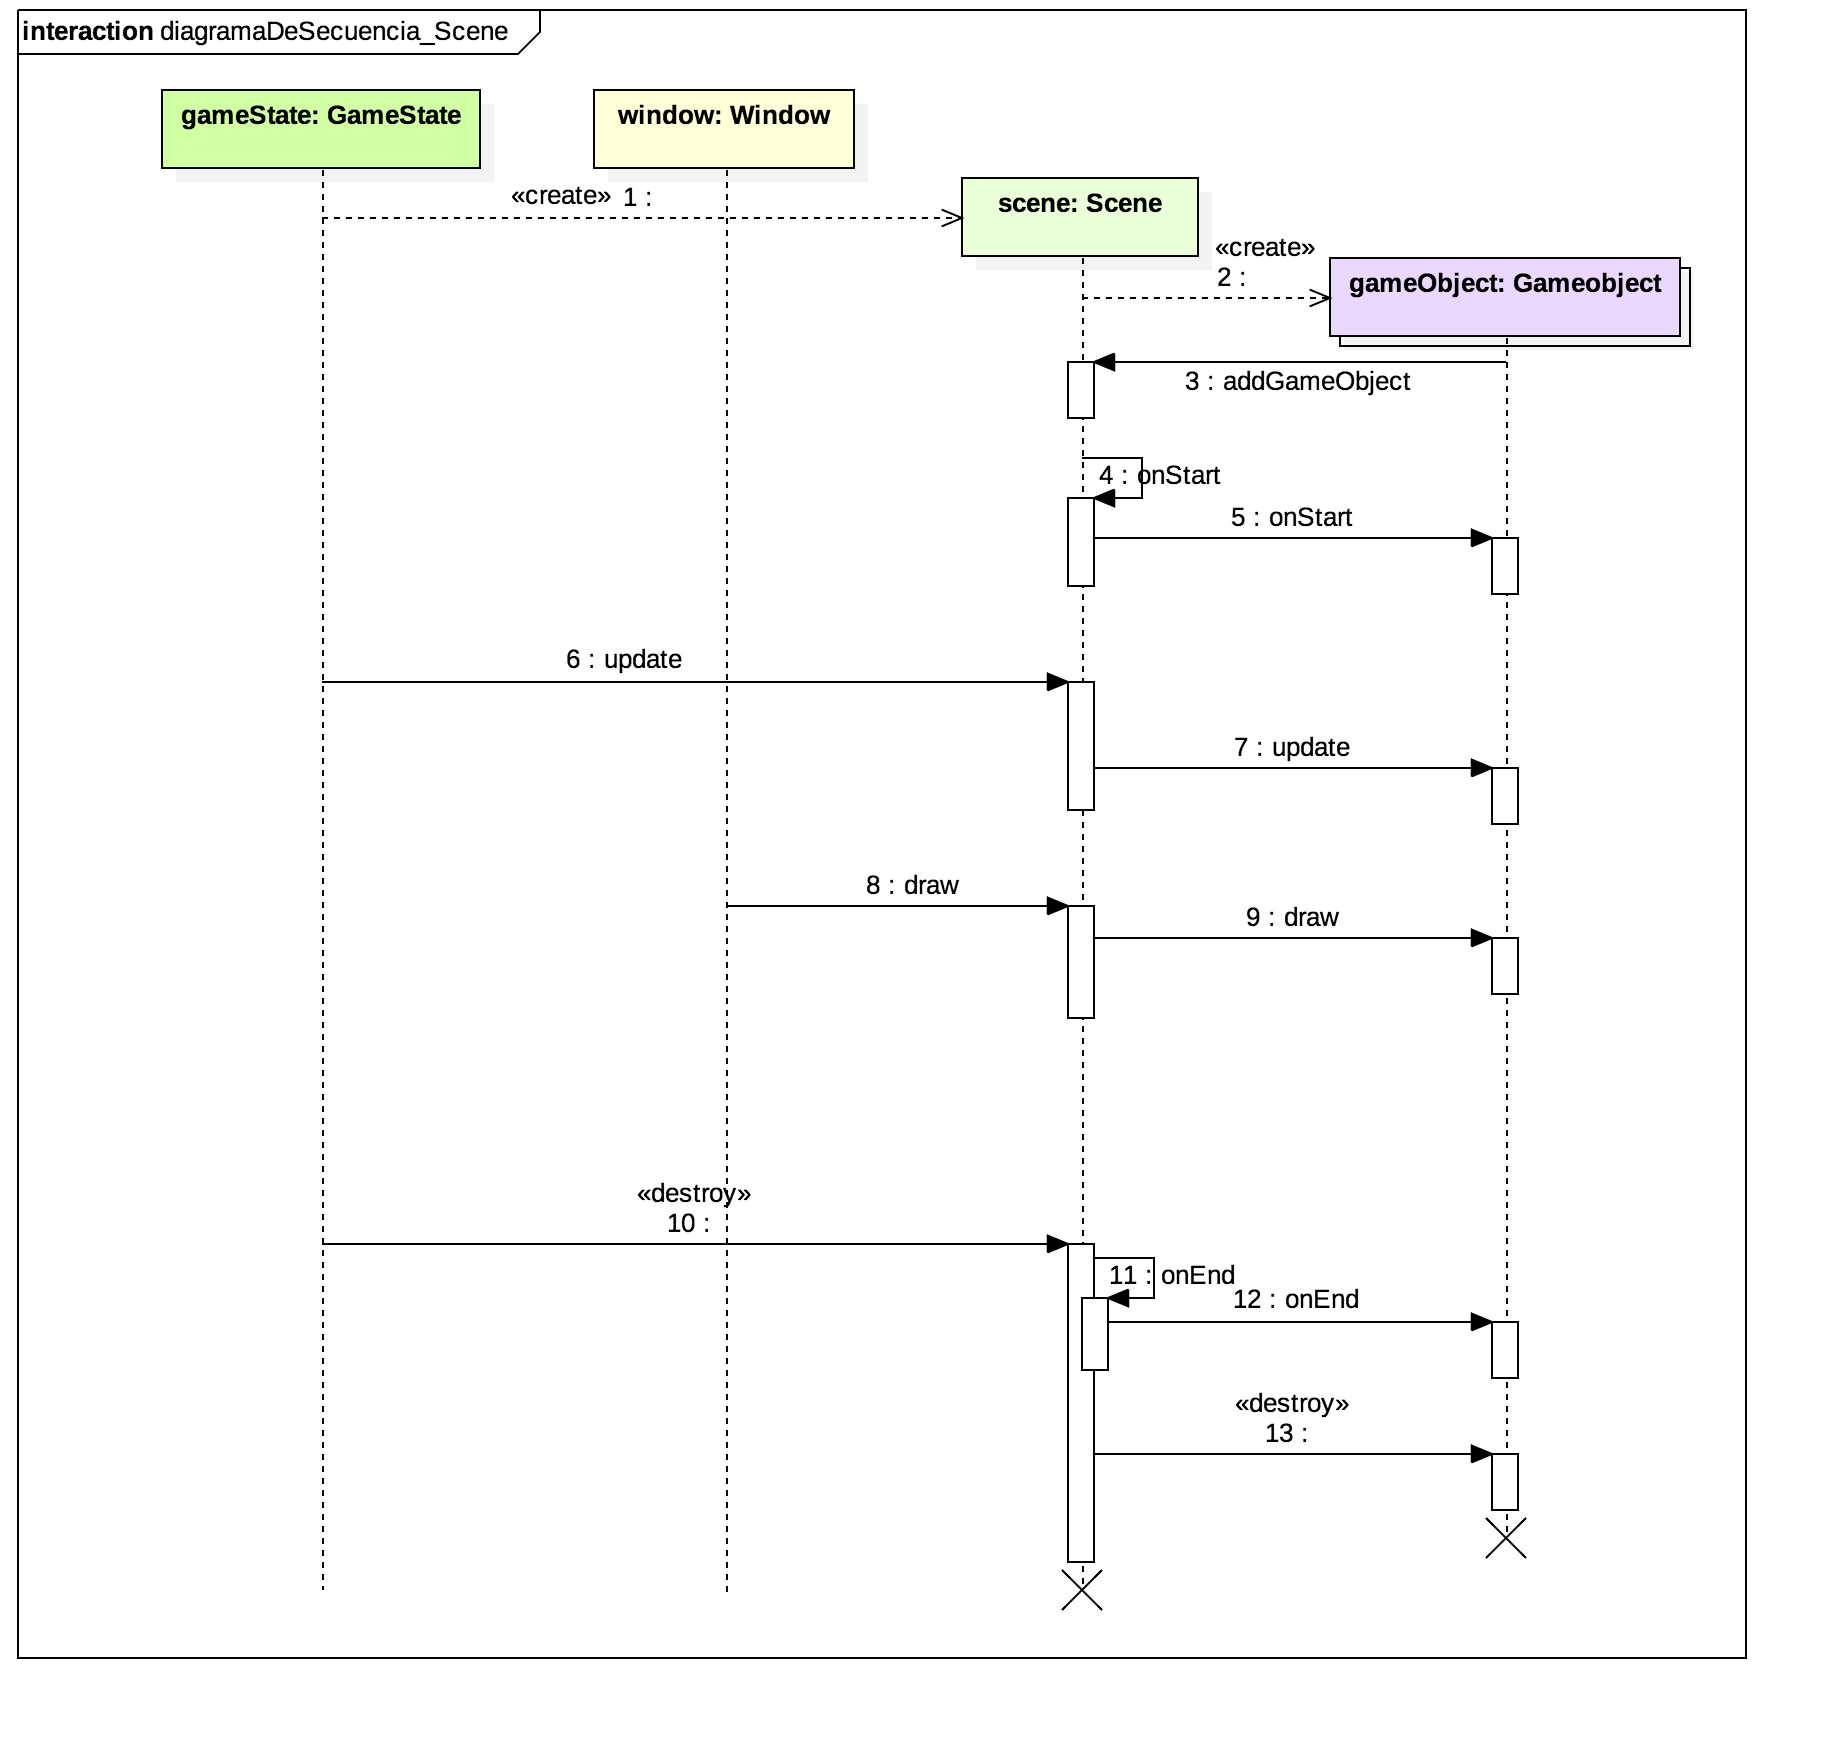
\includegraphics[width=15cm]{otros/UML/png/alld/png/CasosDeUso__General__Collaboration2__Interaction1__diagramaDeSecuencia_Scene_16.png}}
	\caption{Diagrama de secuencia genérico de una escena}
	\label{sec:scene}
\end{figure}

El diagrama de secuencia de la figura \ref{sec:scene} nos muestra como el objeto \textit{gameState} puede crear y destruir una escena para cambiar entre las mismas, lo que se relaciona estrechamente con el CU-3 (seleccionar y ejecutar opción). Además se muestra como es el \textit{gameState} el encargado de actualizar la escena pero será el subsistema de \textit{rendering} con su clase \textit{Window} el encargado de hacer que se dibuje la escena y todos sus \textit{gameobjects}.


\subsubsection*{Consola}

Relacionado estrechamente con el caso de uso CU-9 (Visualizar resultados de combates) y el requisito no funcional RNF-4 (Facilidad para depurar) está el diagrama de secuencia mostrado en la figura \ref{sec:console}.

\bigskip

En orden temporal, se muestra como el usuario puede introducir caracteres por teclado para crear un comando en la consola para luego ejecutarlo y que el mismo se envíe al bus de mensajes. Luego se observa como la clase \textit{Window}, al tener acceso a la consola, es capaz de comprobar si está abierta y dibujarla por pantalla junto con todas las lineas de texto que esta contiene.

\bigskip

Finalmente se muestra como el usuario puede alternar entre visualizar o no la consola al pulsar una determinada tecla interpretada por el sistema de \textit{input}.

\begin{landscape}
\begin{figure}
	\hspace*{-3cm}  
	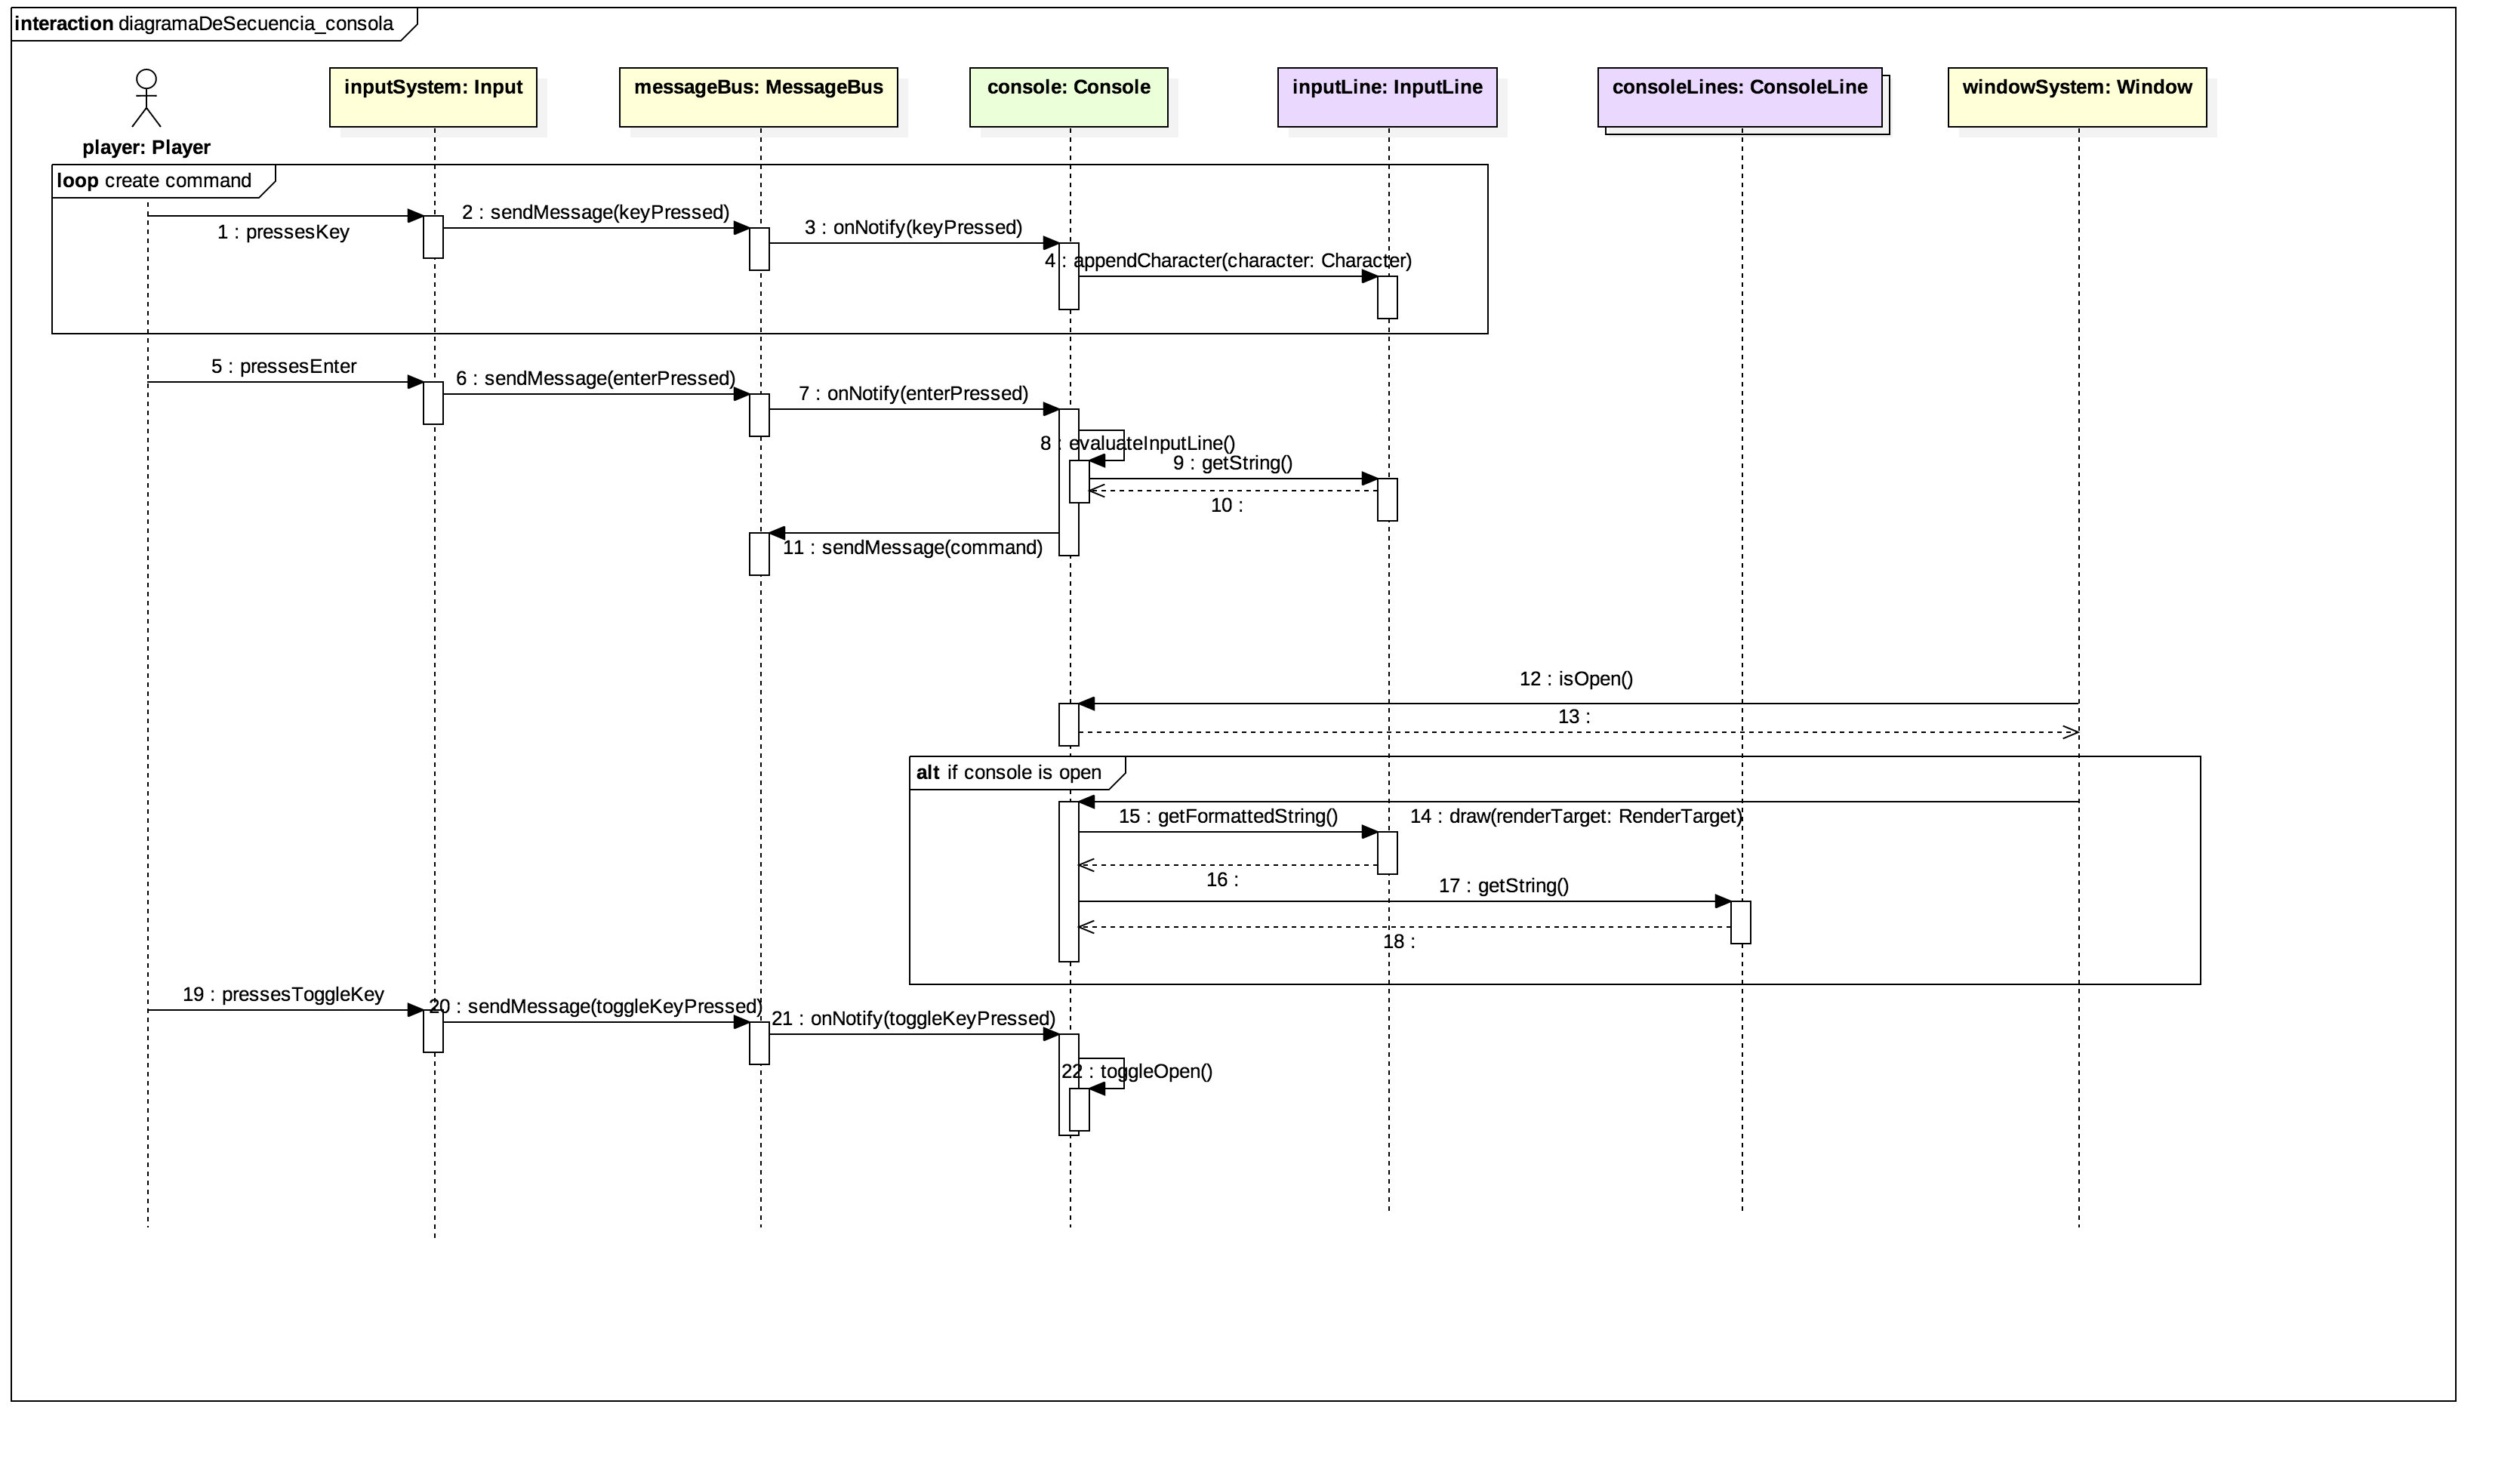
\includegraphics[width=24cm]{otros/UML/png/alld/png/CasosDeUso__Especifico__Collaboration4__Interaction1__diagramaDeSecuencia_consola_20.png}
	\caption{Diagrama de secuencia de la consola}
	\label{sec:console}
\end{figure}
\end{landscape}


\subsection{Escenas y agente}

\subsubsection*{Escena del menú}

En el diagrama de secuencia de la escena del menú de la figura \ref{sec:menu} se ve como el usuario es capaz de seleccionar entre las opciones del menú para luego ejecutar la seleccionada y cambiar de escena.

\bigskip

El flujo comienza por utilizar el sistema de \textit{input} para mandar mensajes referentes a cambiar la opción seleccionada. Una vez que se está en la opción deseada se envía el mensaje de ejecutar dicha opción. En este momento se envía un mensaje que llega al \textit{gameState} indicándole la nueva escena a la que habrá que cambiar, en este momento el \textit{gameState} destruye la escena del menú y genera la nueva escena según la opción seleccionada.

\begin{landscape}
\begin{figure}
	\hspace*{-3cm}  
	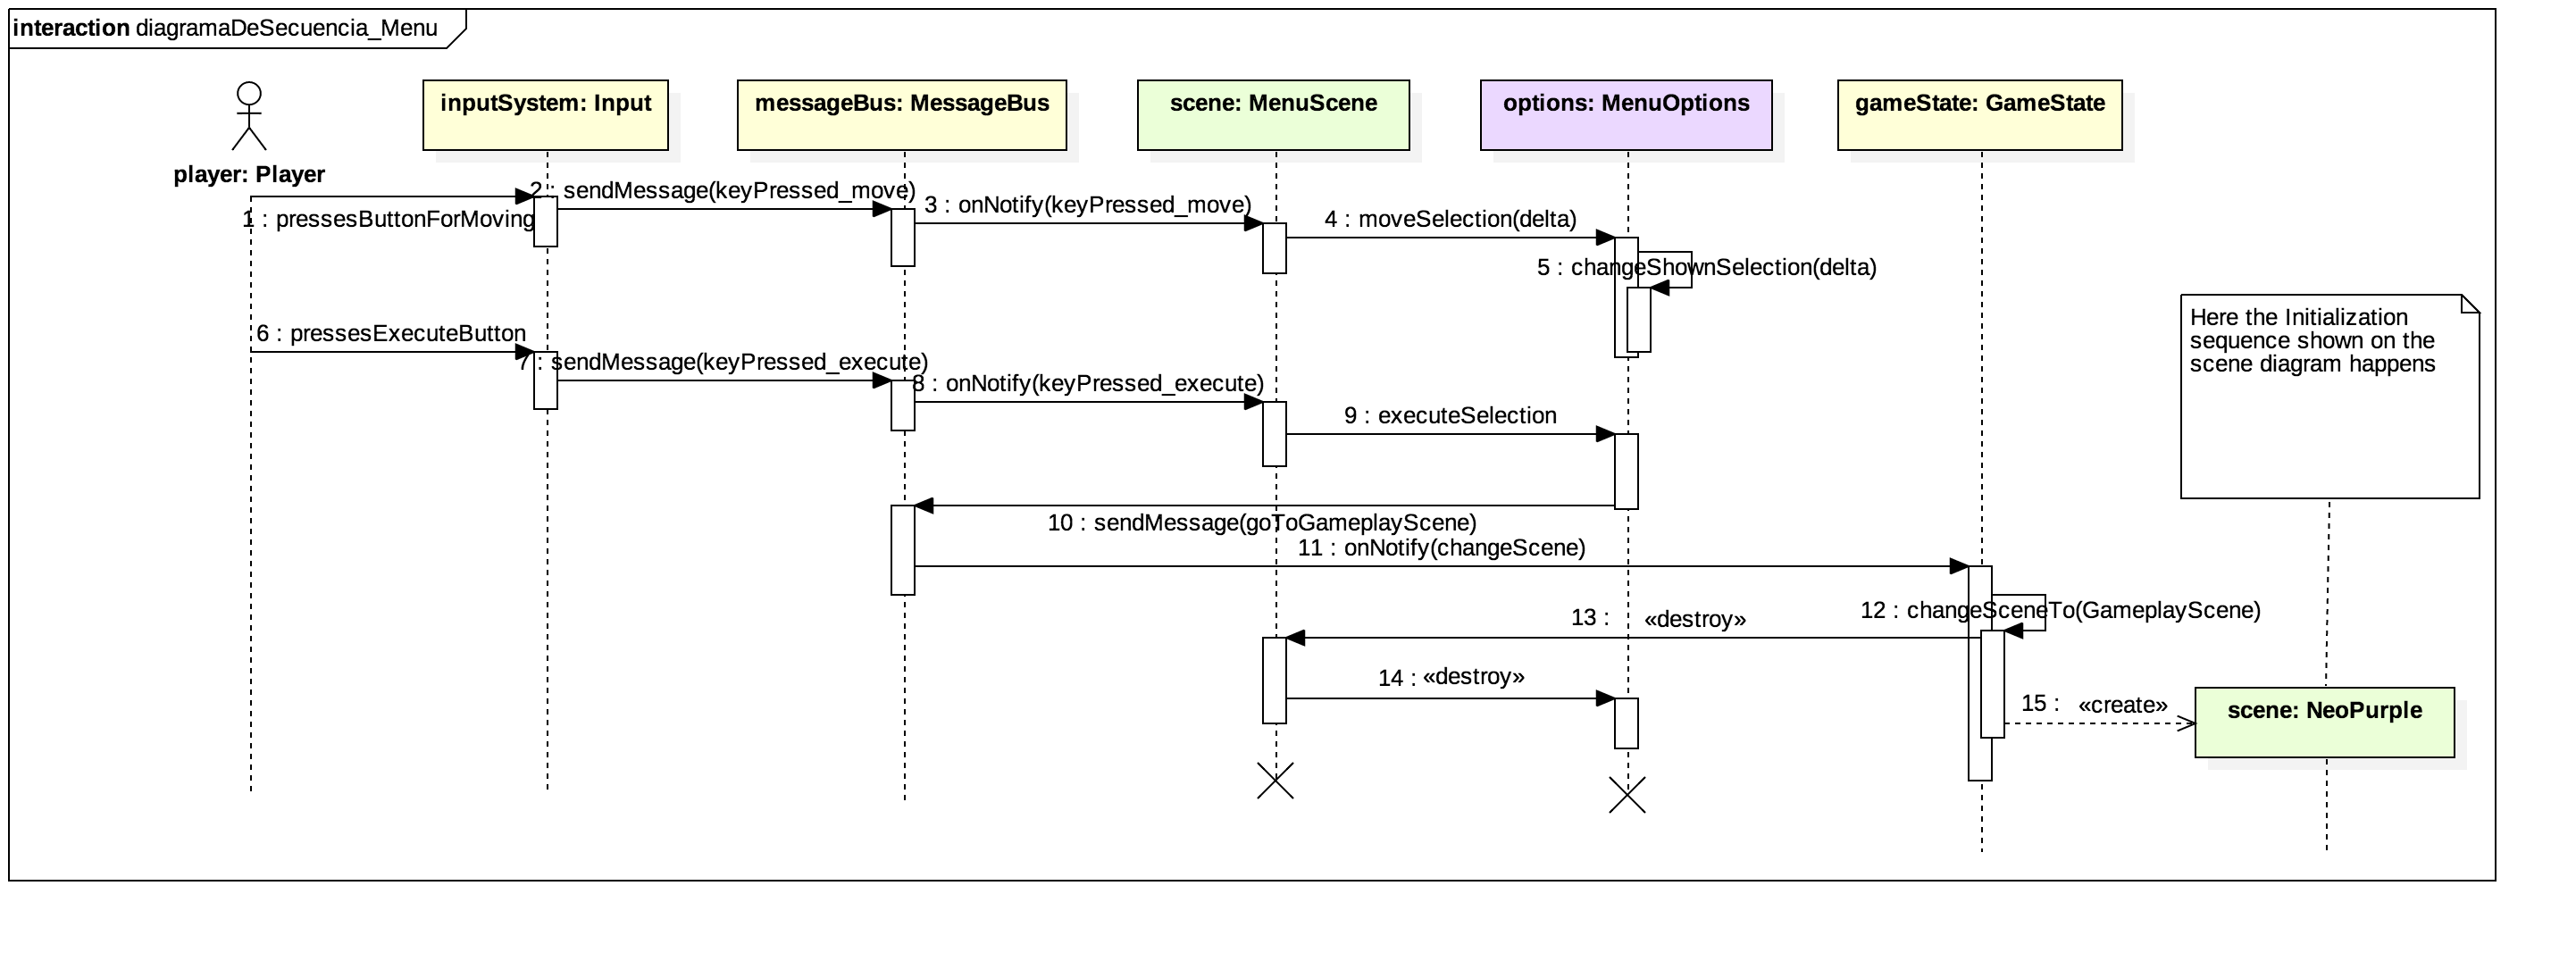
\includegraphics[width=24cm]{otros/UML/png/alld/png/CasosDeUso__Especifico__Collaboration1__Interaction1__diagramaDeSecuencia_Menu_17.png}
	\caption{Diagrama de secuencia de la escena del menú}
	\label{sec:menu}
\end{figure}
\end{landscape}

\subsubsection*{Escena del juego}

La figura \ref{sec:gameplay} contiene el diagrama de secuencia que indica la interacción de un jugador con el videojuego, relacionado con los casos de uso CU-7 (jugador contra agente) y CU-8 (jugador contra jugador).

\bigskip

En el diagrama se muestra como el jugador realiza todas las acciones disponibles para el durante un combate en el siguiente orden temporal:

\begin{enumerate}
	\item El jugador mueve el \textit{joystick} del mando y el mismo se traduce en su personaje moviéndose por la escena.
	\item El jugador pulsa el botón de atacar en el mando y su personaje realiza un ataque.
	\item El jugador pulsa el botón de defenderse y su personaje hace lo propio.
	\item El jugador pulsa el botón de volver al menú, el combate y la escena terminan y se vuelve a la escena del menú.
\end{enumerate}

\begin{figure}
	\centerline{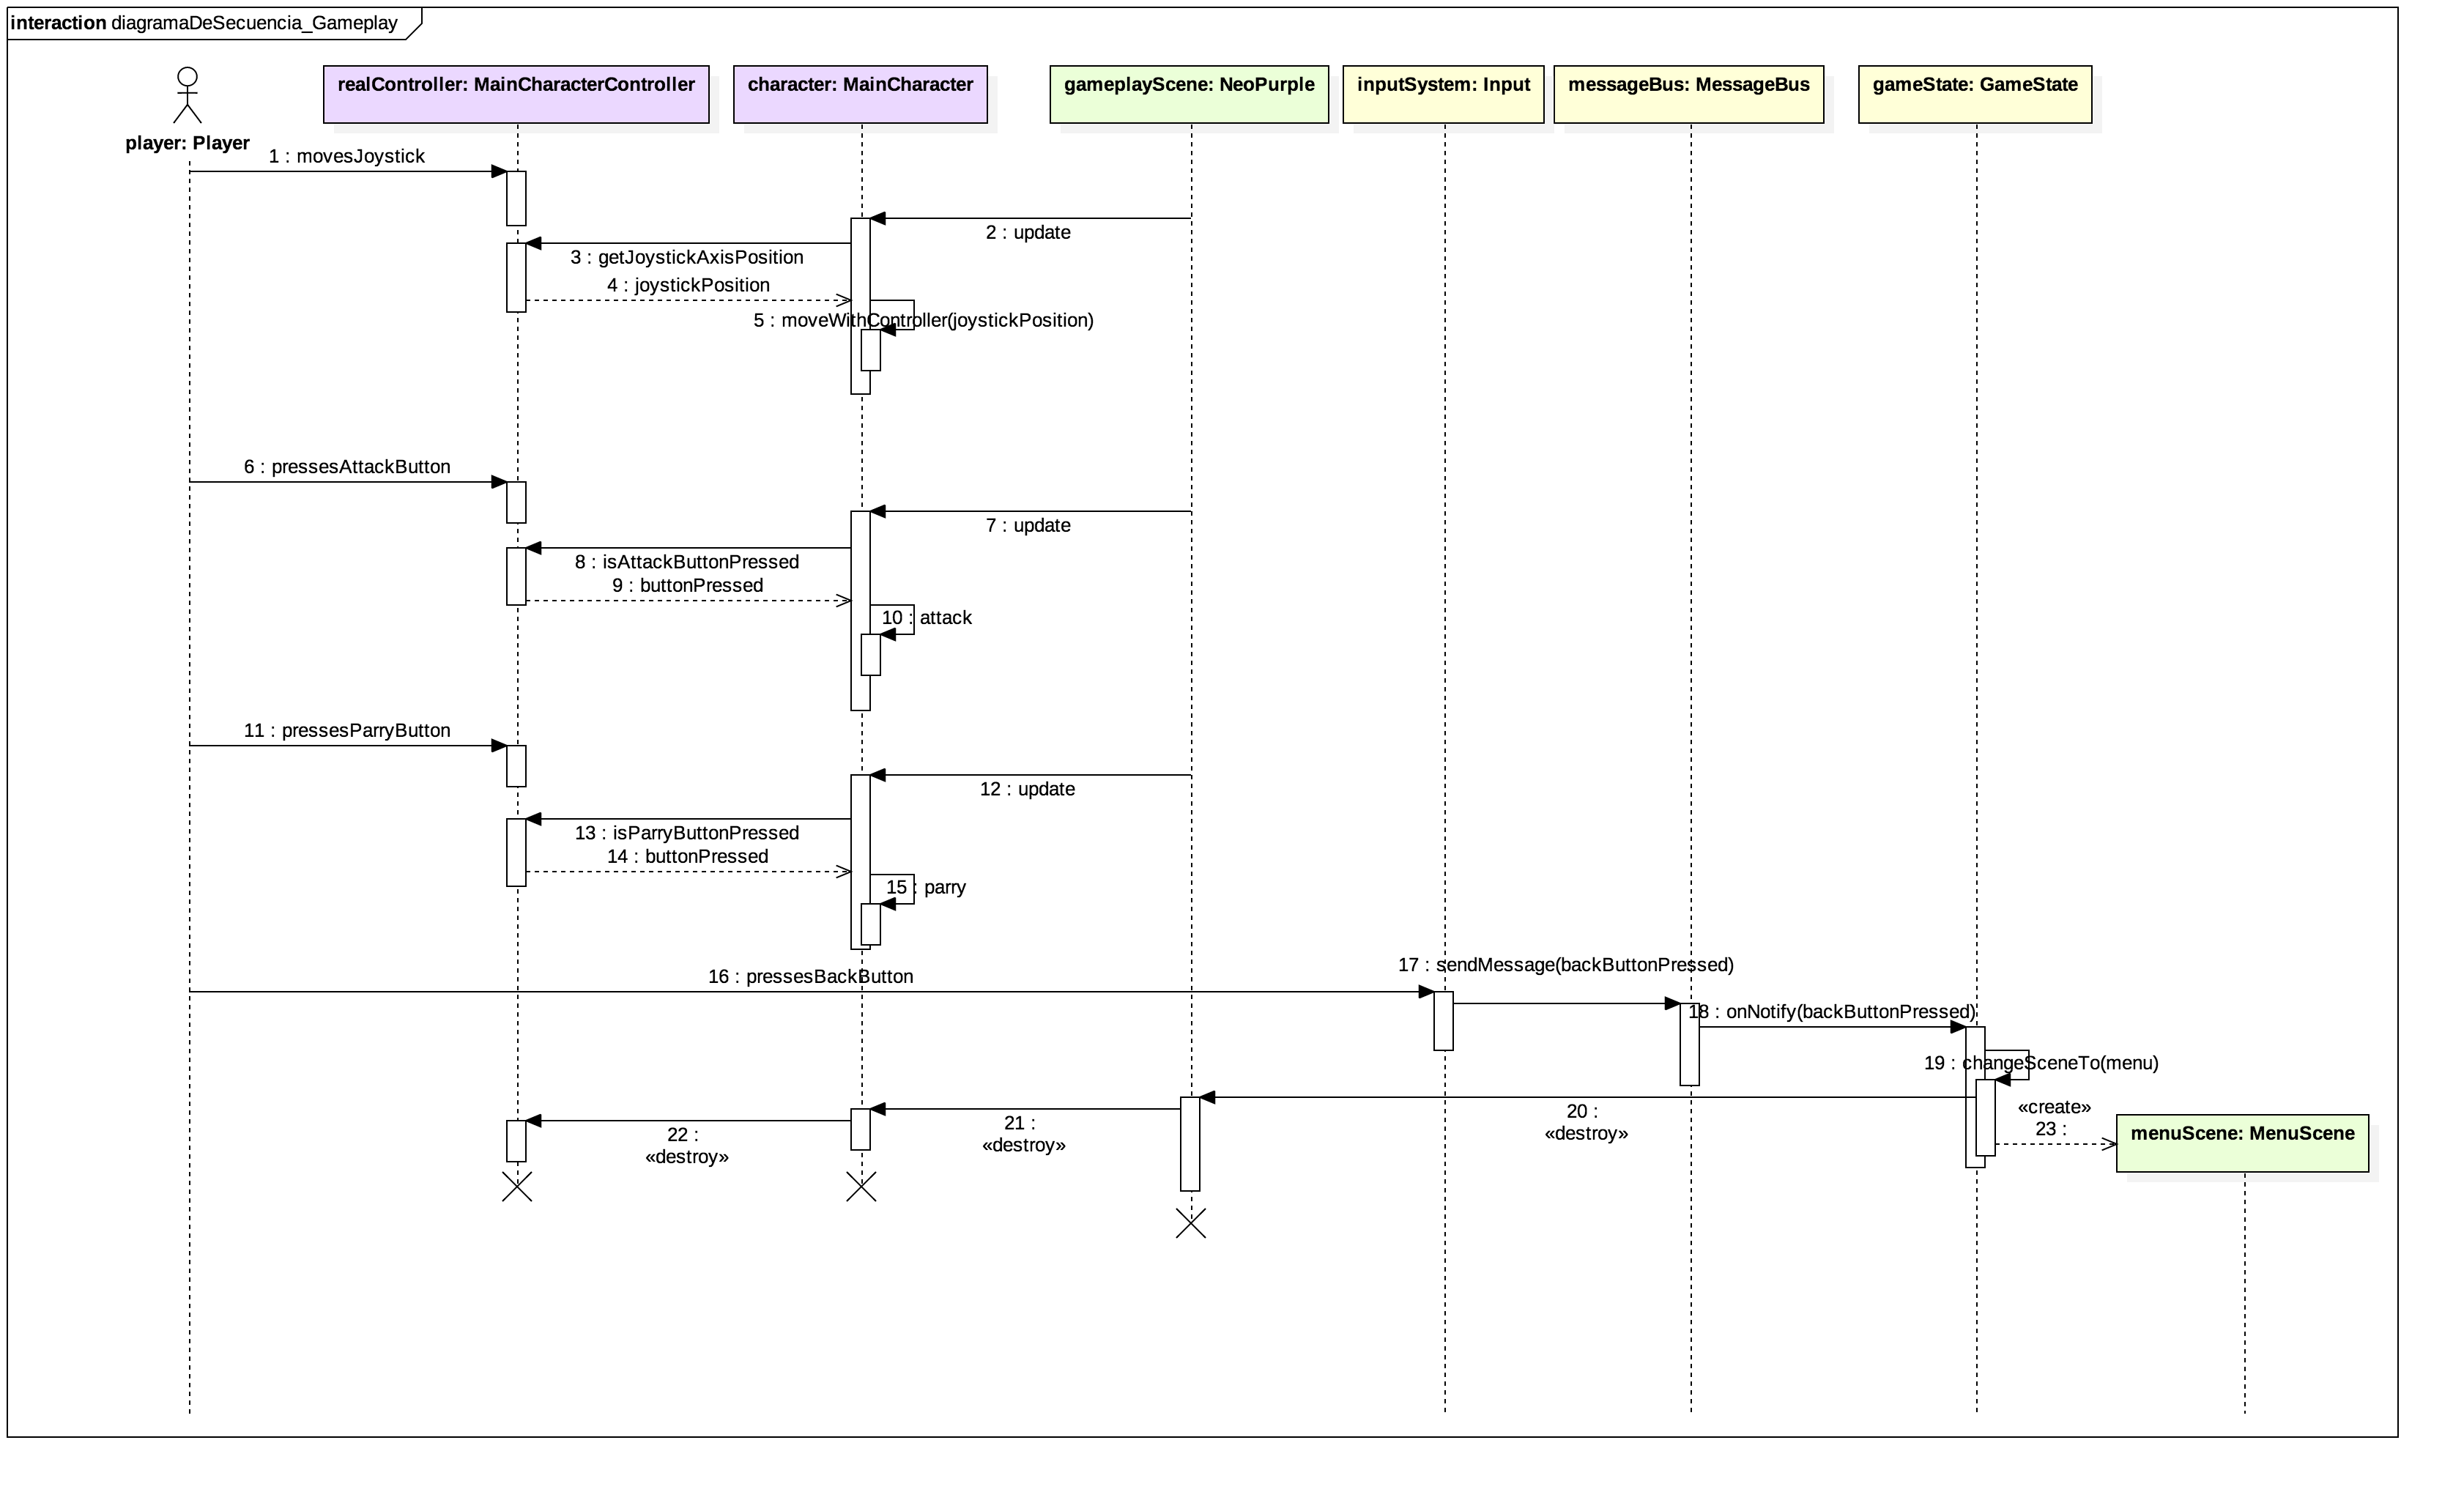
\includegraphics[width=19cm]{otros/UML/png/alld/png/CasosDeUso__Especifico__Collaboration2__Interaction1__diagramaDeSecuencia_Gameplay_18.png}}
	\caption{Diagrama de secuencia de la escena del \textit{gameplay}}
	\label{sec:gameplay}
\end{figure}


\subsubsection*{Agente}


Finalmente, la figura \ref{sec:agent} contiene el diagrama de secuencia asociado al agente y sus acciones. Será más sencillo comprenderlo al relacionarlo con el diagrama de clases del agente mostrado en la figura \ref{class:agent}. Para explicar la secuencia de pasos que se están dando se hace uso de la siguiente enumeración:

\begin{enumerate}
	\item La escena actualiza al agente y este hace lo mismo con su \textit{Observer}.
	\item El comportamiento (\textit{Behaviour}) se actualiza y discretiza el estado continuo mediante el uso del \textit{Observer}.
	\item Se actualiza el conocimiento del agente enviando los datos al \textit{StateActionContainer} y se obtiene del mismo el conocimiento previo sobre el estado actual.
	\item Se calcula la acción a llevar a cabo y se ejecuta con la ayuda de \textit{Actions}. Este objeto modificará el \textit{controller} con los parámetros adecuados.
	\item El personaje leerá los datos del \textit{controller} y ejecutará una de las acciones según el estado de este mando virtual.
\end{enumerate}

\begin{figure}
	\centerline{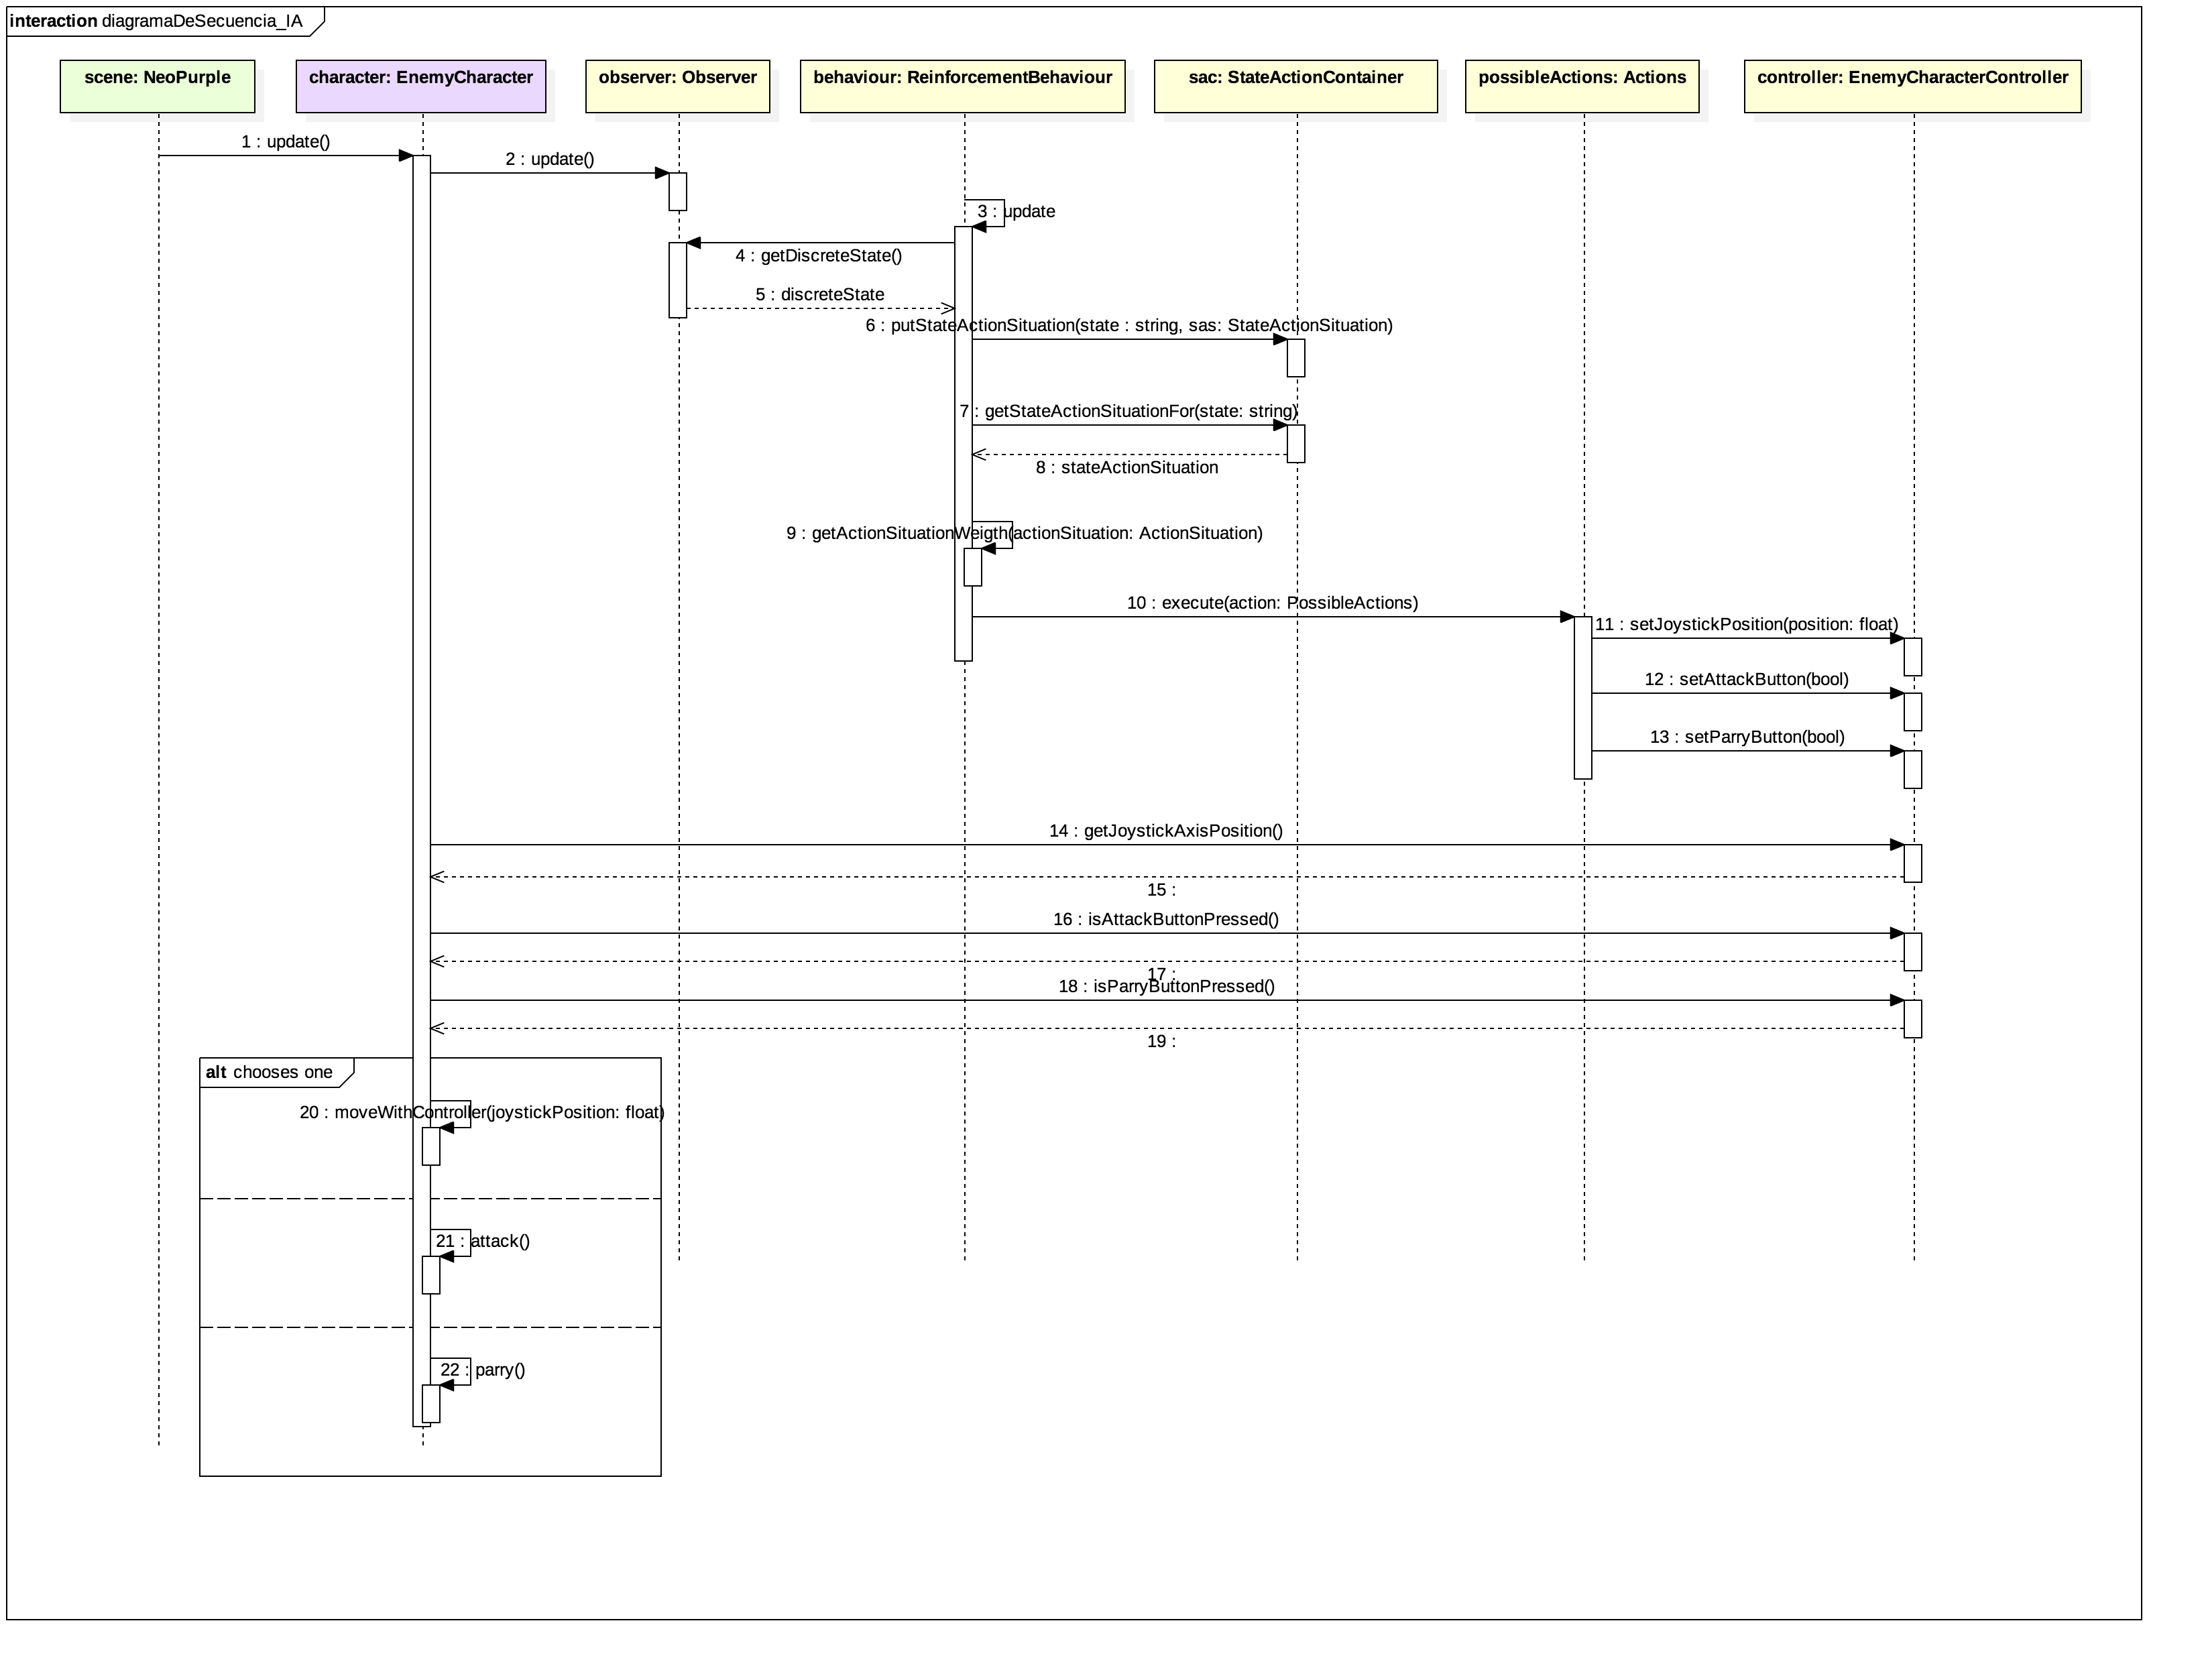
\includegraphics[width=19cm]{otros/UML/png/alld/png/CasosDeUso__Especifico__Collaboration3__Interaction1__diagramaDeSecuencia_IA_19.png}}
	\caption{Diagrama de secuencia del agente}
	\label{sec:agent}
\end{figure}

\section{Diseño de la interfaz gráfica}

Este apartado muestra los diseños realizados primero en papel en referencia a la interfaz gráfica de la aplicación. Dichos diseños son sencillos ya que a diferencia de aplicaciones de otros tipos, los videojuegos de este género suelen optar por evitar una gran cantidad de opciones en una misma vista tendiendo normalmente al minimalismo.

\bigskip

La ventana tendrá una relación de aspecto constante de 4:3 para evocar un parecido con videojuegos antiguos que utilizaban una relación similar dados los estándares de los televisores de la época. Esto debería favorecer la comodidad y dar un aspecto general familiar a los usuarios.

\bigskip

En relación con el requisito no funcional RNF-8 (referente a la usabilidad de la aplicación) se ha buscado la máxima comodidad a la hora de controlar el juego mediante el uso de un mando. Por ello, todos los controles, tanto del menú como del combate están enfocados a ser realizados con un mando similar al de una videoconsola, dejando a un lado el uso del teclado solamente para funciones de depuración o avanzadas tales como abrir y escribir en la consola.

\bigskip

Otro aspecto muy relacionado con la usabilidad es el uso de un indicador sonoro a todas las acciones importantes que se realizan. Dicho indicador tiene que ser constante con la acción que se está mostrando en la interfaz.

\subsection{Interfaz del menú}

En el \textit{mockup}\footnote{modelo de diseño de una interfaz que permite realizar cambios a la misma sin necesidad de implementarla y con el fin de evaluar a grandes rasgos su usabilidad y aspecto} del menú mostrado en la figura \ref{inter:menu} se vé como se ha echo hincapié en la simplicidad del mismo. El título se muestra utilizando un tamaño de fuente superior y las opciones se alinean por la izquierda teniendo en cuenta que pueden tener una longitud distinta.

\bigskip

La opción seleccionada se muestra en negrita y subrayada para no dar lugar a dudas a la hora de distinguirla de las otras. Tanto el cambio entre opciones como la ejecución de una de ellas tienen un sonido asociado lo suficientemente diferente como para ser inconfundibles entre ellos.

\bigskip A la hora de colocar el título y las opciones se ha utilizado la conocida como regla de los tercios\footnote{regla, generalmente asociada a la fotografía, que sugiere que alinear vertical y horizontalmente los elementos de una fotografía con las líneas imaginarias que separa la imagen en tercios las hace más interesantes, naturas y cómodas a la vista}

\begin{figure}
	\centerline{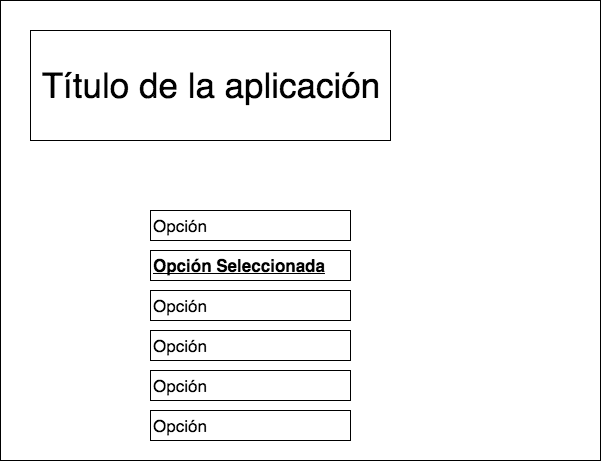
\includegraphics[width=12cm]{otros/graphicalInterface/menu.png}}
	\caption{\textit{Mockup} de la interfaz del menú}
	\label{inter:menu}
\end{figure}

\subsection{Interfaz del combate}

La figura \ref{inter:combat} contiene el \textit{mockup} de la interfaz que el usuario ve al realizar el combate entre personajes. En el mismo se distinguen dos partes diferenciadas:

\bigskip

En la parte superior de la pantalla se ven las barras de vida de los personajes identificadas por colores, dichas barras de vida decrecerán en tamaño horizontalmente para indicar que el personaje asociado ha recibido daño. En el centro se ve un número que indica los segundos restantes del combate, cuando dicho contador llega a cero se termina el combate y gana el jugador con más vida, empatando si es igual. Este tipo de interfaz de combate pretende recordar a la empleada por antiguos juegos de peleas 2D en recreativas tales como \textit{Street Fighter} o \textit{Mortal Kombat} lo que ayuda a que el usuario la considere familiar.

\bigskip

En el centro de la pantalla se puede ver claramente la zona de combate con ambos personajes. Dicha zona se diferencia del resto de la pantalla al utilizar un fondo completamente negro haciendo sencillo el hecho de darse cuenta de que la zona en la que se pueden mover los personajes está limitada. Además los personajes cuentan con un indicador por colores que los relacionan con sus barras de vida para facilitar su identificación durante la batalla.

\bigskip

Durante el combate el hecho de atacar producirá un sonido específico, de la misma forma que recibir daño. Esto incrementa la familiarización del jugador ya que combina la animación mostrada y el sonido con la acción que acaba de ocurrir.

\bigskip

Pese a que no se muestre en la figura, cuando se detiene el combate porque uno de los personajes ha derrotado al otro se muestran letras que indican el jugador ganador, ocupando las mismas toda la pantalla y siendo dibujadas con el mismo color que identifica a cada personaje.

\begin{figure}
	\centerline{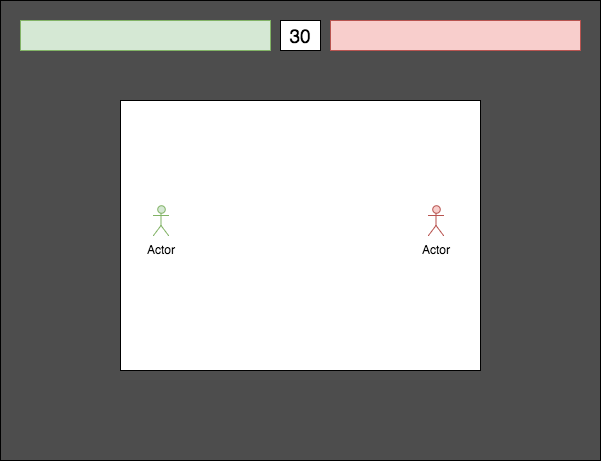
\includegraphics[width=12cm]{otros/graphicalInterface/gameplay.png}}
	\caption{\textit{Mockup} de la interfaz del combate}
	\label{inter:combat}
\end{figure}

\subsection{Interfaz de la consola}

Finalmente, la figura \ref{inter:console} muestra como se vería la consola sobre la aplicación. Recordemos que la misma se puede abrir y cerrar en cualquier escena por lo que tiene un fondo coloreado pero que cierta transparencia que permita ver fácilmente lo que está ocurriendo.

\bigskip

Al fondo de la consola se puede observar una línea con el símbolo $>$ que identifica a la línea de entrada para el usuario. SI la consola está abierta y se escribe en el teclado los caracteres se agregarán a esta línea, siendo limpiada al pulsar \textit{intro}. Las líneas en un negro ligeramente más suave situadas por encima representan los mensajes relevantes que la consola está mostrando al usuario. Finalmente, en la esquina superior izquierda se puede ver un contador de fotogramas por segundo o \textit{FPS}.

\begin{figure}
	\centerline{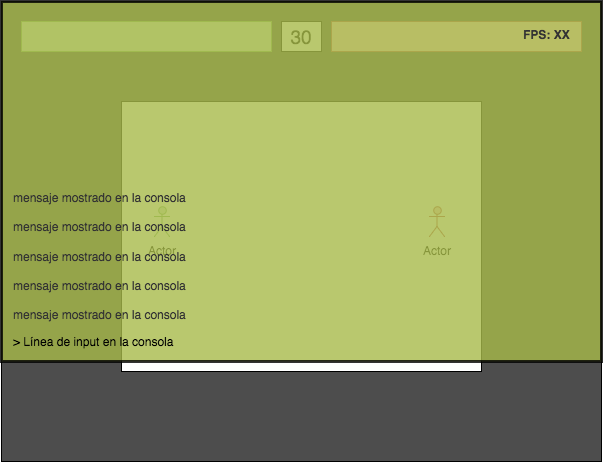
\includegraphics[width=12cm]{otros/graphicalInterface/console.png}}
	\caption{\textit{Mockup} de la interfaz de la consola}
	\label{inter:console}
\end{figure}



\cleardoublepage
\chapter{Validación y pruebas}

Esta sección contiene la documentación asociada a la etapa de validación y pruebas. Su función será comprobar el buen funcionamiento del software y su adecuación con las necesidades del cliente, representadas de modo formal en los requisitos. Para llevar a cabo una serie de pruebas apropiadas se debe prestar especial atención a los criterios de validación especificados para cada requisito, usando los mismos como base para establecer el contenido de cada \textit{test}.

\bigskip

En relación a la metodología utilizada, Programación Extrema, se debe de hacer hincapié en la importancia de la etapa de pruebas ya que constituye uno de los principales aspectos del proyecto. Es también la metodología la que nos ayuda a distinguir entre los siguientes tipos de pruebas:

\begin{itemize}
	\item \textbf{Pruebas Unitarias}: Comprueban que el código de los diferentes componentes se comporta del modo especificado y esperado.
	\item \textbf{Pruebas de Integración}: Comprueban que el sistema funciona correctamente una vez se agrupan los componentes probados de forma unitaria.
	\item \textbf{Pruebas de aceptación o validación del sistema}: Validan que el producto final cumple con las expectativas que el cliente tenía sobre él.
\end{itemize}

Esta separación es especialmente útil dado que la aplicación está significativamente compartimentalizada. Por un lado se encuentran los subsistemas que componen la aplicación que se conectan entre sí y por otro el agente que interactúa con la aplicación. La realización de las pruebas en el orden especificado ayudará a comprobar individualmente los diferentes módulos del sistema para luego integrarlos y poden verificar el comportamiento del mismo como un todo. Una vez finalizado se debe validar el producto en su conjunto para tener la seguridad de que se cumplen as expectativas.

\bigskip

En los siguientes apartados se describen las pruebas llevadas a cabo relacionándolas con el elemento que las ha originado si este existe.

\section{Pruebas unitarias}

Este apartado contiene las pruebas asociadas a cada requisito, sea este funcional o no. Por su parte, los requisitos de información no generarán en pruebas de ningún tipo ya que el correcto funcionamiento del almacenamiento de datos se realiza de forma indirecta con el conjunto de pruebas realizado para los otros tipos de requisitos.

\subsection{Requisitos funcionales}

Las pruebas unitarias referentes a los requisitos funcionales siguen el estándar de nombrado con la forma \textit{\textbf{PU\_RF-N}}, siendo \textbf{\textit{N}} el número asociado.

\newcounter{contador_pruebas_funcionales}
\setcounter{contador_pruebas_funcionales}{1}

\begin{center}
	\begin{tabular}{ | p{3cm} | p{10cm} | } 
		\hline
		
		\textbf{ID} & PU\_RF-\arabic{contador_pruebas_funcionales}
		\refstepcounter{contador_pruebas_funcionales} \\
		
		\hline 
		\textbf{ID de RF} &
		RF-1: Visualización del menú\\ 
		
		\hline
		\textbf{Descripción} & 
		Se busca llegar al menú usando todas las formas posibles que incluyen:
		\begin{itemize}
			\item Entrar en la aplicación
			\item Terminar el combate con un ganador
			\item Forzar la salida del combate 
		\end{itemize}\\
		
		\hline 
		\textbf{Resultado esperado} &
		Se visualiza el menú correctamente en todas las situaciones.\\ 
		
		\hline 
		\textbf{Estado} &
		Cumplido\\ 
		
		\hline
	\end{tabular}
\end{center}

\begin{center}
	\begin{tabular}{ | p{3cm} | p{10cm} | } 
		\hline
		
		\textbf{ID} & PU\_RF-\arabic{contador_pruebas_funcionales}
		\refstepcounter{contador_pruebas_funcionales} \\
		
		\hline 
		\textbf{ID de RF} &
		RF-2: Moverse en el menú\\ 
		
		\hline
		\textbf{Descripción} & 
		Se intenta utilizar tanto el mando como las flechas del teclado para moverse arriba y abajo en las opciones del menú.\\
		
		\hline 
		\textbf{Resultado esperado} &
		Aún utilizando ambos métodos de entrada a la vez la opción se mueve arriba y abajo una vez por tecla pulsada. Apareciendo la selección al inicio si se mueve abajo en la última opción y al final si se mueve la selección arriba en la primera opción.\\ 
		
		\hline 
		\textbf{Estado} &
		Cumplido\\ 
		
		\hline
	\end{tabular}
\end{center}

\begin{center}
	\begin{tabular}{ | p{3cm} | p{10cm} | } 
		\hline
		
		\textbf{ID} & PU\_RF-\arabic{contador_pruebas_funcionales}
		\refstepcounter{contador_pruebas_funcionales} \\
		
		\hline 
		\textbf{ID de RF} &
		RF-2: Moverse en el menú\\ 
		
		\hline
		\textbf{Descripción} & 
		Se comprueba que la opción mostrada como preseleccionada se corresponde siempre con la acción ejecutada al pulsar el botón de lanzar la opción. Se probará con cada una de las opciones, llegando a la misma moviendo la selección solo para arriba, abajo y las dos formas.\\
		
		\hline 
		\textbf{Resultado esperado} &
		Siempre que se seleccione una misma opción esta ejecuta la misma escena, siendo esta la indicada en el nombre de la opción.\\ 
		
		\hline 
		\textbf{Estado} &
		Cumplido\\ 
		
		\hline
	\end{tabular}
\end{center}

\begin{center}
	\begin{tabular}{ | p{3cm} | p{10cm} | } 
		\hline
		
		\textbf{ID} & PU\_RF-\arabic{contador_pruebas_funcionales}
		\refstepcounter{contador_pruebas_funcionales} \\
		
		\hline 
		\textbf{ID de RF} &
		RF-3: Ejecutar una opción del menú\\ 
		
		\hline
		\textbf{Descripción} & 
		Se ejecutan cada una de las opciones del menú en los distintos estados del juego:
		\begin{itemize}
			\item Se acaba de entrar en la aplicación
			\item Se acaba de terminar el combate con un ganador
			\item Se acaba de forzar la salida del combate 
		\end{itemize}\\
		
		\hline 
		\textbf{Resultado esperado} &
		Todas las opciones siguen llevando siempre a la ejecución correcta de la escena asociada a cada una de ellas.\\ 
		
		\hline 
		\textbf{Estado} &
		Cumplido\\ 
		
		\hline
	\end{tabular}
\end{center}

\begin{center}
	\begin{tabular}{ | p{3cm} | p{10cm} | } 
		\hline
		
		\textbf{ID} & PU\_RF-\arabic{contador_pruebas_funcionales}
		\refstepcounter{contador_pruebas_funcionales} \\
		
		\hline 
		\textbf{ID de RF} &
		RF-4: Alternar apertura de consola con resultados\\ 
		
		\hline
		\textbf{Descripción} & 
		Se intenta abrir y cerrar la consola durante la ejecución de la escena del menú y durante todos los tipos de combate.\\
		
		\hline 
		\textbf{Resultado esperado} &
		Se abre, visualiza y cierra correctamente la consola en todos los casos excepto en el caso de simulación sin \textit{renderizado} en el cual no se muestra nada.\\ 
		
		\hline 
		\textbf{Estado} &
		Cumplido\\ 
		
		\hline
	\end{tabular}
\end{center}

\begin{center}
	\begin{tabular}{ | p{3cm} | p{10cm} | } 
		\hline
		
		\textbf{ID} & PU\_RF-\arabic{contador_pruebas_funcionales}
		\refstepcounter{contador_pruebas_funcionales} \\
		
		\hline 
		\textbf{ID de RF} &
		RF-5: Salir de la aplicación\\ 
		
		\hline
		\textbf{Descripción} & 
		Se cierra la aplicación utilizando la funcionalidad propia del sistema de ventanas de macOS (\textbf{Control + Q} o pulsando la \textbf{X roja}) en todas las escenas de la misma. Además se usa la opción del menú indicada para cerrar el programa.\\
		
		\hline 
		\textbf{Resultado esperado} &
		La aplicación se cierra sin errores en todos los casos y se ejecuta correctamente la próxima vez que se abre.\\ 
		
		\hline 
		\textbf{Estado} &
		Cumplido\\ 
		
		\hline
	\end{tabular}
\end{center}

\begin{center}
	\begin{tabular}{ | p{3cm} | p{10cm} | } 
		\hline
		
		\textbf{ID} & PU\_RF-\arabic{contador_pruebas_funcionales}
		\refstepcounter{contador_pruebas_funcionales} \\
		
		\hline 
		\textbf{ID de RF} &
		RF-6: Entrar en la escena de combate\\ 
		
		\hline
		\textbf{Descripción} & 
		Se usan cada una de las cuatro opciones del menú para pasar a la escena de combate y se controla al personaje en las opciones de jugador contra jugador y jugador contra agente.\\
		
		\hline 
		\textbf{Resultado esperado} &
		Todas las opciones hacen que se entre en la escena correctamente y se puede controlar al jugador solamente en las dos opciones mencionadas.\\ 
		
		\hline 
		\textbf{Estado} &
		Cumplido\\ 
		
		\hline
	\end{tabular}
\end{center}

\begin{center}
	\begin{tabular}{ | p{3cm} | p{10cm} | } 
		\hline
		
		\textbf{ID} & PU\_RF-\arabic{contador_pruebas_funcionales}
		\refstepcounter{contador_pruebas_funcionales} \\
		
		\hline 
		\textbf{ID de RF} &
		RF-7: Moverse en el área de combate\\ 
		
		\hline
		\textbf{Descripción} & 
		Se usan las dos opciones de jugador contra jugador y jugador contra agente. Luego, se intenta mover al personaje con el \textit{joystick} del mando. Usando dos mandos en la primera opción para mover a ambos personajes\\
		
		\hline 
		\textbf{Resultado esperado} &
		El personaje se mueve en la dirección esperada en todos los casos\\ 
		
		\hline 
		\textbf{Estado} &
		Cumplido\\ 
		
		\hline
	\end{tabular}
\end{center}

\begin{center}
	\begin{tabular}{ | p{3cm} | p{10cm} | } 
		\hline
		
		\textbf{ID} & PU\_RF-\arabic{contador_pruebas_funcionales}
		\refstepcounter{contador_pruebas_funcionales} \\
		
		\hline 
		\textbf{ID de RF} &
		RF-8: Atacar al enemigo\\ 
		
		\hline
		\textbf{Descripción} & 
		Se intenta atacar al enemigo cuando este está a rango, cuando no lo está y cuando está a rango pero el personaje no está orientado hacia él. Se realiza el proceso tanto para un personaje como para el otro.\\
		
		\hline 
		\textbf{Resultado esperado} &
		Siempre que el enemigo está a rango, estamos mirando hacia él y no se está defendiendo el mismo sufre daño. En cualquier otro caso no es dañado.\\ 
		
		\hline 
		\textbf{Estado} &
		Cumplido\\ 
		
		\hline
	\end{tabular}
\end{center}

\begin{center}
	\begin{tabular}{ | p{3cm} | p{10cm} | } 
		\hline
		
		\textbf{ID} & PU\_RF-\arabic{contador_pruebas_funcionales}
		\refstepcounter{contador_pruebas_funcionales} \\
		
		\hline 
		\textbf{ID de RF} &
		RF-9: Defenderse del enemigo\\ 
		
		\hline
		\textbf{Descripción} & 
		Se realiza una defensa ante el ataque del otro personaje y cuando este no está atacando. Además se ataca al personaje durante el periodo de defensa e inmediatamente después. Se repite el proceso para ambos personajes.\\
		
		\hline 
		\textbf{Resultado esperado} &
		Si el personaje se está defendiendo nunca sufre daño, al ser atacado en otro caso sí es dañado.\\ 
		
		\hline 
		\textbf{Estado} &
		Cumplido\\ 
		
		\hline
	\end{tabular}
\end{center}

\begin{center}
	\begin{tabular}{ | p{3cm} | p{10cm} | } 
		\hline
		
		\textbf{ID} & PU\_RF-\arabic{contador_pruebas_funcionales}
		\refstepcounter{contador_pruebas_funcionales} \\
		
		\hline 
		\textbf{ID de RF} &
		RF-10: Ganar perder partida\\ 
		
		\hline
		\textbf{Descripción} & 
		Se hace que ambos personajes sufran daño suficiente para que su vida llegue a cero en todas las escenas posibles. Se comprueba que no es posible que ambos ganen en el mismo fotograma.\\
		
		\hline 
		\textbf{Resultado esperado} &
		El personaje que no tiene la vida a cero es nombrado el ganador en todos los casos. Si ambos atacan en el mismo fotograma solo uno de ellos será el ganador.\\ 
		
		\hline 
		\textbf{Estado} &
		Cumplido\\ 
		
		\hline
	\end{tabular}
\end{center}

\begin{center}
	\begin{tabular}{ | p{3cm} | p{10cm} | } 
		\hline
		
		\textbf{ID} & PU\_RF-\arabic{contador_pruebas_funcionales}
		\refstepcounter{contador_pruebas_funcionales} \\
		
		\hline 
		\textbf{ID de RF} &
		RF-11: Agotar el tiempo de combate\\ 
		
		\hline
		\textbf{Descripción} & 
		Se hace que el tiempo disponible de combate llegue a cero en todas las escenas de combate posibles.\\
		
		\hline 
		\textbf{Resultado esperado} &
		Se vuelve al menú correctamente, marcando como ganador al personaje con más vida en el momento en el que se termina el tiempo y no nombrando un ganador si su vira era la misma.\\ 
		
		\hline 
		\textbf{Estado} &
		Cumplido\\ 
		
		\hline
	\end{tabular}
\end{center}

\begin{center}
	\begin{tabular}{ | p{3cm} | p{10cm} | } 
		\hline
		
		\textbf{ID} & PU\_RF-\arabic{contador_pruebas_funcionales}
		\refstepcounter{contador_pruebas_funcionales} \\
		
		\hline 
		\textbf{ID de RF} &
		RF-12: Volver al menú\\ 
		
		\hline
		\textbf{Descripción} & 
		En las escenas de combate con visualización se intenta volver al menú pulsando el botón determinado para ello.\\
		
		\hline 
		\textbf{Resultado esperado} &
		Siempre se vuelve correctamente al menú de la aplicación sin nombrar como ganador a ninguno de los personajes.\\ 
		
		\hline 
		\textbf{Estado} &
		Cumplido\\ 
		
		\hline
	\end{tabular}
\end{center}

\begin{center}
	\begin{tabular}{ | p{3cm} | p{10cm} | } 
		\hline
		
		\textbf{ID} & PU\_RF-\arabic{contador_pruebas_funcionales}
		\refstepcounter{contador_pruebas_funcionales} \\
		
		\hline 
		\textbf{ID de RF} &
		RF-13: Visualizar combates entre agentes\\ 
		
		\hline
		\textbf{Descripción} & 
		Se utiliza la opción de agente contra agente en la que se puede ver un combate entre dos enemigos.\\
		
		\hline 
		\textbf{Resultado esperado} &
		Los dos personajes combaten entre sí sin que sea necesaria ninguna interacción por parte del usuario.\\ 
		
		\hline 
		\textbf{Estado} &
		Cumplido\\ 
		
		\hline
	\end{tabular}
\end{center}

\begin{center}
	\begin{tabular}{ | p{3cm} | p{10cm} | } 
		\hline
		
		\textbf{ID} & PU\_RF-\arabic{contador_pruebas_funcionales}
		\refstepcounter{contador_pruebas_funcionales} \\
		
		\hline 
		\textbf{ID de RF} &
		RF-14: Simular múltiples combates\\ 
		
		\hline
		\textbf{Descripción} & 
		Se utiliza la opción de agente contra agente sin visualización en la que dos enemigos combaten entre sí múltiples veces de forma iterativa.\\
		
		\hline 
		\textbf{Resultado esperado} &
		No se visualiza nada durante unos segundos y se vuelve al menú, pudiendo ver los datos de victorias de ambos personajes en la consola.\\ 
		
		\hline 
		\textbf{Estado} &
		Cumplido\\ 
		
		\hline
	\end{tabular}
\end{center}

\begin{center}
	\begin{tabular}{ | p{3cm} | p{10cm} | } 
		\hline
		
		\textbf{ID} & PU\_RF-\arabic{contador_pruebas_funcionales}
		\refstepcounter{contador_pruebas_funcionales} \\
		
		\hline 
		\textbf{ID de RF} &
		RF-15: Comandos en la consola\\ 
		
		\hline
		\textbf{Descripción} & 
		Se introducen mensajes en la consola de la aplicación que algunos o todos los subsistemas entienden y mensajes que no están contemplados por la aplicación.\\
		
		\hline 
		\textbf{Resultado esperado} &
		Todos los subsistemas que deban responder a un mensaje lo hacen, si el mensaje no es soportado por ninguno de los subsistemas entonces no ocurre nada.\\ 
		
		\hline 
		\textbf{Estado} &
		Cumplido\\ 
		
		\hline
	\end{tabular}
\end{center}



\subsection{Requisitos no funcionales}

Las pruebas unitarias referentes a los requisitos no funcionales siguen el estándar de nombrado con la forma \textit{\textbf{PU\_RNF-N}}, siendo \textbf{\textit{N}} el número asociado.

\newcounter{contador_pruebas_no_funcionales}
\setcounter{contador_pruebas_no_funcionales}{1}

\begin{center}
	\begin{tabular}{ | p{3cm} | p{10cm} | } 
		\hline
		
		\textbf{ID} & PU\_RNF-\arabic{contador_pruebas_no_funcionales}
		\refstepcounter{contador_pruebas_no_funcionales} \\
		
		\hline 
		\textbf{ID de RF} &
		RNF-1: Rendimiento de la aplicación\\ 
		
		\hline
		\textbf{Descripción} & 
		Se realizarán un total de 10 combates de cada tipo (obviando el que no es visualizado) en dos equipos distintos y se observará el contador de fotogramas por segundo mostrado en la consola.\\
		
		\hline 
		\textbf{Resultado esperado} &
		En ningún momento los fotogramas por segundo caen por debajo de 59.\\
		
		\hline 
		\textbf{Estado} &
		Cumplido\\ 
		
		\hline
	\end{tabular}
\end{center}

\begin{center}
	\begin{tabular}{ | p{3cm} | p{10cm} | } 
		\hline
		
		\textbf{ID} & PU\_RNF-\arabic{contador_pruebas_no_funcionales}
		\refstepcounter{contador_pruebas_no_funcionales} \\
		
		\hline 
		\textbf{ID de RF} &
		RNF-2: Velocidad de las simulaciones\\
		
		\hline
		\textbf{Descripción} & 
		Se realizan una serie de simulaciones de forma iterativa midiendo al final el tiempo empleado para todas ellas y calculando el tiempo medio por simulación.\\
		
		\hline 
		\textbf{Resultado esperado} &
		Se pueden realizar combates enteros simulados en un tiempo medio inferior a 100 milisegundos.\\
		
		\hline 
		\textbf{Estado} &
		Cumplido (media de 38 milisegundos por simulación)\\ 
		
		\hline
	\end{tabular}
\end{center}

\begin{center}
	\begin{tabular}{ | p{3cm} | p{10cm} | } 
		\hline
		
		\textbf{ID} & PU\_RNF-\arabic{contador_pruebas_no_funcionales}
		\refstepcounter{contador_pruebas_no_funcionales} \\
		
		\hline 
		\textbf{ID de RF} &
		RNF-3: Extensibilidad del motor\\
		
		\hline
		\textbf{Descripción} & 
		Se comprueba la dificultad de añadir un nuevo subsistema a la arquitectura existente (realizado con el subsistema de sonido).\\
		
		\hline 
		\textbf{Resultado esperado} &
		No se tiene que modificar ninguna otra parte de la aplicación excepto simplemente añadir los mensajes que indican que se llame al nuevo subsistema (mensajes para reproducir cada sonido).\\
		
		\hline 
		\textbf{Estado} &
		Cumplido\\ 
		
		\hline
	\end{tabular}
\end{center}

\begin{center}
	\begin{tabular}{ | p{3cm} | p{10cm} | } 
		\hline
		
		\textbf{ID} & PU\_RNF-\arabic{contador_pruebas_no_funcionales}
		\refstepcounter{contador_pruebas_no_funcionales} \\
		
		\hline 
		\textbf{ID de RF} &
		RNF-4: Facilidad para depurar\\
		
		\hline
		\textbf{Descripción} & 
		Se marcan los mensajes de la aplicación como relevantes para la consola y se hace que la misma los muestre cuando está abierta.\\
		
		\hline 
		\textbf{Resultado esperado} &
		Se visualizan fácilmente los mensajes en tiempo de ejecución en la consola integrada sin tener que acudir a la consola del IDE o del sistema.\\
		
		\hline 
		\textbf{Estado} &
		Cumplido\\ 
		
		\hline
	\end{tabular}
\end{center}

\begin{center}
	\begin{tabular}{ | p{3cm} | p{10cm} | } 
		\hline
		
		\textbf{ID} & PU\_RNF-\arabic{contador_pruebas_no_funcionales}
		\refstepcounter{contador_pruebas_no_funcionales} \\
		
		\hline 
		\textbf{ID de RF} &
		RNF-5: Aplicación autocontenida\\
		
		\hline
		\textbf{Descripción} & 
		Se ejecuta la aplicación en un equipo distinto del de desarrollo sin realizar ninguna instalación previa. Además se realiza una instalación limpia del sistema en una máquina virtual y se prueba que el programa funciona.\\
		
		\hline 
		\textbf{Resultado esperado} &
		La aplicación se ejecuta correctamente en ambos entornos sin necesitar de recursos adicionales.\\
		
		\hline 
		\textbf{Estado} &
		Cumplido\\ 
		
		\hline
	\end{tabular}
\end{center}

\begin{center}
	\begin{tabular}{ | p{3cm} | p{10cm} | } 
		\hline
		
		\textbf{ID} & PU\_RNF-\arabic{contador_pruebas_no_funcionales}
		\refstepcounter{contador_pruebas_no_funcionales} \\
		
		\hline 
		\textbf{ID de RF} &
		RNF-6: Extensibilidad en términos de escenas\\
		
		\hline
		\textbf{Descripción} & 
		Se añade temporalmente una escena a la que se entra desde el menú y se sale pulsando cualquier botón (La escena no está disponible en la versión final pues solo se crea con fines de prueba).\\
		
		\hline 
		\textbf{Resultado esperado} &
		Añadir y eliminar la escena no implica ningún cambio en el resto de la aplicación más que permitir entrar en ella desde otra escena.\\
		
		\hline 
		\textbf{Estado} &
		Cumplido\\ 
		
		\hline
	\end{tabular}
\end{center}

\begin{center}
	\begin{tabular}{ | p{3cm} | p{10cm} | } 
		\hline
		
		\textbf{ID} & PU\_RNF-\arabic{contador_pruebas_no_funcionales}
		\refstepcounter{contador_pruebas_no_funcionales} \\
		
		\hline 
		\textbf{ID de RF} &
		RNF-7: Documentación\\
		
		\hline
		\textbf{Descripción} & 
		Se revisa la documentación en busca de secciones que no aporten información, lo hagan de forma deficiente o dupliquen la misma innecesariamente.\\
		
		\hline 
		\textbf{Resultado esperado} &
		No se encuentran apartados con los errores descritos.\\
		
		\hline 
		\textbf{Estado} &
		Cumplido\\ 
		
		\hline
	\end{tabular}
\end{center}

\begin{center}
	\begin{tabular}{ | p{3cm} | p{10cm} | } 
		\hline
		
		\textbf{ID} & PU\_RNF-\arabic{contador_pruebas_no_funcionales}
		\refstepcounter{contador_pruebas_no_funcionales} \\
		
		\hline 
		\textbf{ID de RF} &
		RNF-8: Usabilidad de la interfaz\\
		
		\hline
		\textbf{Descripción} & 
		Se hace que cinco usuarios ejecuten por primera vez la aplicación una vez observada la sección de controles del mando del manual de usuario\ref{sec:controles}.\\
		
		\hline 
		\textbf{Resultado esperado} &
		Más de 3 de los 5 usuarios califican la aplicación como usable en una escala del entre 1 y 5, considerando como usable una puntuación de 4 o superior.\\
		
		\hline 
		\textbf{Estado} &
		Cumplido: 4 de los 5 usuarios han puntuado con más de un 4 mientras 1 de ellos ha puntuado con un 3 por tener dificultades al diferenciar entre el botón de atacar y el de seleccionar opción del menú.\\ 
		
		\hline
	\end{tabular}
\end{center}


\section{Pruebas de integración}

Una vez tratadas las pruebas unitarias en referencia a los requisitos individuales de la aplicación se dedica este apartado a comprobar cada unión de los componentes que no ha sido probada todavía de forma indirecta durante las pruebas unitarias.

\bigskip

Llegados a este punto se necesitarán hacer modificaciones sobre la aplicación para realizar algunas de las pruebas de integración. Estos cambios no estarán presentes en la versión final dado que en muchas ocasiones requieren recursos computacionales adicionales que no se pueden desperdiciar.

\bigskip

Las pruebas de integración seguirán un estándar de nombrado con la forma \textbf{\textit{PI-N}} siendo \textbf{\textit{N}} su número asociado.

\newcounter{contador_pruebas_integracion}
\setcounter{contador_pruebas_integracion}{1}

\begin{center}
	\begin{tabular}{ | p{3cm} | p{10cm} | } 
		\hline
		
		\textbf{ID} & PI-\arabic{contador_pruebas_integracion}
		\refstepcounter{contador_pruebas_integracion} \\
	
		\hline
		\textbf{Descripción} & 
		Se comprobará que todos los sistemas pueden comunicarse con cualquier otro mandando desde cada uno de ellos un mensaje general para todos los otros y luego un mensaje específico a cada uno de ellos, incluyéndose a si mismo.\\
		
		\hline 
		\textbf{Resultado esperado} &
		Todos los subsistemas reciben todos los mensajes generales enviados y los que son específicos para ellos mismos, sea cual sea el origen o el contenido.\\
		
		\hline 
		\textbf{Estado} &
		Cumplido\\ 
		
		\hline
	\end{tabular}
\end{center}

\begin{center}
	\begin{tabular}{ | p{3cm} | p{10cm} | } 
		\hline
		
		\textbf{ID} & PI-\arabic{contador_pruebas_integracion}
		\refstepcounter{contador_pruebas_integracion} \\
		
		\hline
		\textbf{Descripción} & 
		Se comprueba que el agente es capaz de realizar cualquier acción en la escena de combate. Para ello se hace que elija iterativamente entre todas las acciones disponibles y se observa como se llevan a cabo en la escena.\\
		
		\hline 
		\textbf{Resultado esperado} &
		Al realizar cualquier acción especificada, el movimiento y situación del personaje controlado por el agente cambia de forma apropiada.\\
		
		\hline 
		\textbf{Estado} &
		Cumplido\\ 
		
		\hline
	\end{tabular}
\end{center}

\begin{center}
	\begin{tabular}{ | p{3cm} | p{10cm} | } 
		\hline
		
		\textbf{ID} & PI-\arabic{contador_pruebas_integracion}
		\refstepcounter{contador_pruebas_integracion} \\
		
		\hline
		\textbf{Descripción} & 
		Se comprueba que no hay diferencias entre los combates simulados y no simulados excepto la velocidad a la que transcurren. Para ello se escribe un \textit{log} que indica la posición en cada bucle del programa de los dos personajes y de su situación y se comparan los \textit{logs} obtenidos simulando y sin simular. Para evitar que cambie el comportamiento dados los parámetros aleatorios se especifica la misma raíz al comenzar los combates.\\
		
		\hline 
		\textbf{Resultado esperado} &
		Los \textit{logs} indican que no hay diferencias entre combates simulados y no simulados (a tiempo real).\\ 
		
		\hline 
		\textbf{Estado} &
		Cumplido\\ 
		
		\hline
	\end{tabular}
\end{center}

\begin{center}
	\begin{tabular}{ | p{3cm} | p{10cm} | } 
		\hline
		
		\textbf{ID} & PI-\arabic{contador_pruebas_integracion}
		\refstepcounter{contador_pruebas_integracion} \\
		
		\hline
		\textbf{Descripción} & 
		Se comprueba que el agente siempre es capaz de acceder a su archivo de \textit{conocimiento} integrado en la aplicación y si este no existe crea uno y guarda en el mismo los datos. Para ello se eliminará el archivo existente y se ejecutará la aplicación.\\
		
		\hline 
		\textbf{Resultado esperado} &
		Siempre se accede al archivo si este existe. Sino se crea uno y se pobla con los datos aprendidos.\\
		
		\hline 
		\textbf{Estado} &
		Cumplido\\ 
		
		\hline
	\end{tabular}
\end{center}

\section{Validación del agente}
\label{sec:valicacion}
Las etapas anteriores referidas a las pruebas unitarias y a las pruebas de integración demuestran el correcto funcionamiento de la aplicación y del agente integrado en la misma. Esta sección se dedica a validar al agente en referencia al objetivo general del proyecto, es decir, a ser capaces de competir simulando un comportamiento eficaz y realista.

\bigskip

Por razones temporales y por que se saldría del alcance de este proyecto, no es posible realizar un proceso con una cantidad suficiente de pruebas en las que se examine, registre y analice el comportamiento del agente contra una cantidad suficiente de jugadores humanos.

\bigskip

Para hacer esto posible se debería disponer de grupos relativamente numerosos sin experiencia en el juego y compuestos por jugadores de distintos niveles de experiencia en videojuegos de este estilo. Esto es difícil de conseguir y gestionar, además de que supondría un consumo de tiempo importante.

\bigskip

Sin embargo, pruebas realizadas con un pequeño conjunto de jugadores indican que la implementación del personaje controlado por la aplicación basado en reglas supone un comportamiento similar al de un jugador real. Esto sumado a la capacidad del motor para simular combates entre personajes controlados por la máquina hace que el método más eficaz y eficiente de obtener datos sea realizar dichas simulaciones.

\bigskip

En este sentido, se realizarán 100 simulaciones en las que se enfrentarán agentes entrenados de diferentes modos y el personaje basado en reglas, obteniendo así una aproximación de las capacidades del mismo al enfrentarse en un futuro a jugadores reales. El porcentaje de victorias mostrado en los cuadros se obtiene de estas 100 simulaciones independientes realizadas en cada preciso momento del entrenamiento.

\bigskip

Los siguientes apartados contendrán los datos referentes al comportamiento del agente entrenado de diferentes formas:

\begin{itemize}
	\item \textbf{Agente 1}: Entrenado contra el personaje basado en reglas.
	\item \textbf{Agente 2}: Entrenado contra otra instancia de él mismo.
\end{itemize}

\subsection{Entrenado contra personaje basado en reglas (Agente 1)}
\label{agente1}
\begin{table}
	\begin{center}
		\begin{tabular}{c|c|c|c|c|c|c|}
			& \multicolumn{6}{c|}{\textbf{Numero de simulaciones de entrenamiento}:}\\
			\cline{2-7} & \textbf{0} & \textbf{100} & \textbf{1000} & \textbf{5000} & \textbf{10000} & \textbf{20000}\\
			
			\hline
			\textbf{Victorias (en \%)}: &  15 & 25 & 48 & 49 & 76 & 70\\
			
			\hline
		\end{tabular}
		\caption{Rendimiento del agente entrenado contra personaje basado en reglas}
		\label{rend:reglas:victorias}
	\end{center}
\end{table}

\begin{table}
	\begin{center}
		\begin{tabular}{c|c|c|c|c|c|c|}
			& \multicolumn{6}{c|}{\textbf{Numero de simulaciones de entrenamiento}:}\\
			\cline{2-7} & \textbf{0} & \textbf{100} & \textbf{1000} & \textbf{5000} & \textbf{10000} & \textbf{20000}\\
			
			\hline
			\textbf{Estados visitados}: &  6596 & 10940 & 23887 & 36588 & 42162 & 47699 \\
			
			\hline
		\end{tabular}
		\caption{Estados visitados por el agente entrenado contra personaje basado en reglas}
		\label{rend:reglas:estados}
	\end{center}
\end{table}

Como se puede observar en la tabla \ref{rend:reglas:victorias}, el agente entrenado contra el personaje basado en reglas en aproximadamente unos 1000 combates es capaz de competir con el rendimiento suficiente como para empatar. Llegados ya a 5000 combates simulados, el agente aprende cómo pelear de forma muy efectiva contra el personaje basado en reglas.

\bigskip

De forma interesante, al continuar con el entrenamiento su comportamiento se vuelve ligeramente peor, una posible explicación es que una vez se exploran demasiado algunos estados se priorizan acciones que pueden no ser las idóneas.

\bigskip

En lo que corresponde a la tabla de estados visitados (\ref{rend:reglas:estados}) se observa que existe un límite en lo que se refiere a los estados que presenta el personaje basado en reglas. Este límite está cercano a los 50000 estados como se ha comprobado con entrenamiento posterior. Esto se debe a que al comportarse según unas reglas definidas con poca aleatoriedad, las situaciones a las que da lugar también son limitadas. Se estima que la combinación total de estados es de \textbf{194400} teniendo en cuenta todas las combinaciones de variables de los estados discretos.

\subsection{Entrenado contra él mismo (Agente 2)}
\label{agente2}
\label{cap:pruebas:mismo}

\begin{table}
	\begin{center}
		\begin{tabular}{c|c|c|c|c|c|c|}
			& \multicolumn{6}{c|}{\textbf{Numero de simulaciones de entrenamiento}:}\\
			\cline{2-7} & \textbf{0} & \textbf{100} & \textbf{1000} & \textbf{5000} & \textbf{10000} & \textbf{20000}\\
			
			\hline
			\textbf{Victorias (en \%)}: &  13 & 33 & 40 & 60 & 61 & 54\\
			
			\hline
		\end{tabular}
		\caption{Rendimiento del agente entrenado contra otra instancia de si mismo}
		\label{rend:el:victorias}
	\end{center}
\end{table}

\begin{table}
	\begin{center}
		\begin{tabular}{c|c|c|c|c|c|c|}
			& \multicolumn{6}{c|}{\textbf{Numero de simulaciones de entrenamiento}:}\\
			\cline{2-7} & \textbf{0} & \textbf{100} & \textbf{1000} & \textbf{5000} & \textbf{10000} & \textbf{20000}\\
			
			\hline
			\textbf{Estados visitados}: &  6767 & 24231 & 50659 & 66523 & 73908 & 79371 \\
			
			\hline
		\end{tabular}
		\caption{Estados visitados por el agente entrenado contra otra instancia de si mismo}
		\label{rend:el:estados}
	\end{center}
\end{table}

Pasando ahora al agente entrenado contra él mismo, uno de los aspectos más importantes es que al tener dos instancias del agente que comparten el mismo conocimiento, en entrenamiento es el doble de efectivo ya que los dos aprenden a la vez. Esto se observa en la tabla \ref{rend:el:estados} llegando a un máximo de estados rozando 80000.

\bigskip

Otra de las razones por la cual se visitan tantos estados a mayores es que se responde a situaciones menos comunes generadas por el agente que no sabe como comportarse en un estado. De esta forma la variabilidad en el comportamiento es significativa, sobre todo en las primeras simulaciones.

\bigskip

En lo que corresponde a la tabla \ref{rend:el:victorias}, vemos que el agente no es tan efectiva como el entrenado contra reglas. Esto es perfectamente lógico ya que el otro agente tiene mucha más experiencia contra el mismo.


\section{Comparación y elección del agente final}

\begin{figure}
	\centerline{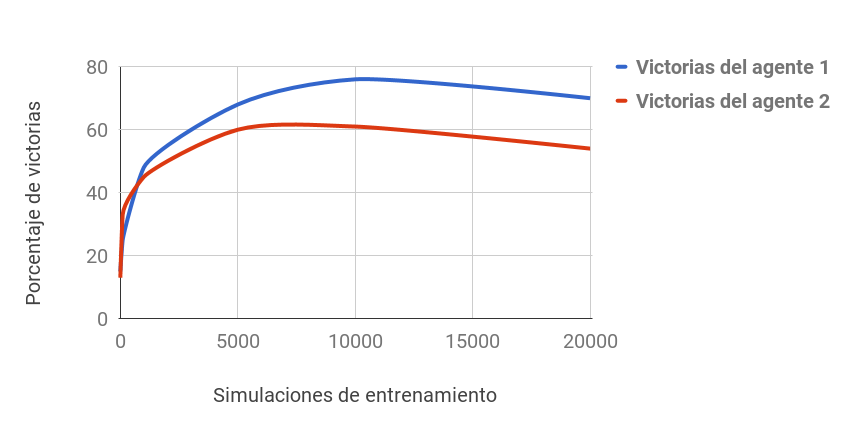
\includegraphics[width=15cm]{otros/otrasCapturas/grafico_victorias.png}}
	\caption{Porcentaje de victorias contra el personaje basado en reglas}
	\label{graf:victorias}
\end{figure}

\begin{figure}
	\centerline{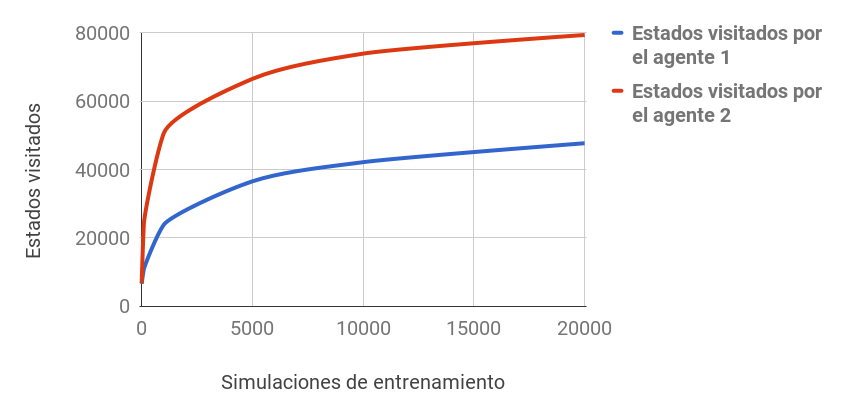
\includegraphics[width=15cm]{otros/otrasCapturas/grafico_estados.png}}
	\caption{Estados visitados durante el entrenamiento}
	\label{graf:estados}
\end{figure}

En comparación, el que llamaremos \textbf{agente 1} explicado en la sección \ref{agente1} es significativamente mejor que el \textbf{agente 2} referenciado en la sección \ref{agente2} al competir contra un personaje basado en reglas como se puede observar en la gráfica contenida en la figura \ref{graf:victorias}. Una de las razones más importantes que lleva a esto es que el agente 2, al realizar cada uno de los grupos de 100 combates para obtener las estadísticas, está peleando por primera vez contra el personaje pasado en reglas, por lo que no está tan especializado en las situaciones que se dan.

\bigskip

Por otra parte, como se puede ver en el gráfico de la figura \ref{graf:estados}, hay que tener en cuenta que el agente 2 es significativamente superior en lo que a exploración del espacio de estados se refiere. Esto genera un comportamiento mucho más completo contra jugadores humanos ya que las situaciones que los mismos crean pueden llegar a ser extremadamente raras para el agente 1. Al haber visitado más estados se responde de forma más efectiva a oponentes con patrones poco frecuentes.

\bigskip

Algo importante que se ha observado sobre el agente 2 es que al principio de su entrenamiento, si se realizan combates contra él, su respuesta es mala comparada con la del agente 1. Esto se debe a que como entrena contra él mismo, tarda más que el agente 1 en empezar a saber que acciones son las mejores.

\bigskip

Lo que nos lleva a la \textbf{elección} del agente que se presentará en la versión final de la aplicación. Dicho agente empezará su entrenamiento contra el personaje basado en reglas para evitar ese lento comienzo que se menciona en el párrafo anterior. Luego pasará a entrenar contra él mismo para favorecer una exploración máxima de estados, el resultado es un agente con una frecuencia de victorias estimada del \textbf{80\%} y una cantidad de estados visitados de \textbf{75407}.

\bigskip

Esto favorece que la versión final presentada contenga un agente que sabe tanto responder a estados poco comunes como elegir la mejor acción en situaciones frecuentes.

\section{Observaciones}

Al analizar el comportamiento del agente elegido se han observado comportamientos relativamente complejos que no se esperaban en un principio. Algunos de los que comentaremos a continuación se pueden ver en un vídeo subido a \textit{YouTube}\footnote{disponible en: \url{https://youtu.be/NdtrxdUIRWw}} en el que el agente es en todas las ocasiones el \textbf{jugador o \textit{player} 2} identificado con el color \textbf{rojo}.

\bigskip

El agente suele emplear una estrategia agresiva para comenzar el combate con ventaja. Se observa como es capaz de anticiparse a cuando el enemigo estará a rango atacando primero y posicionándose en una buena situación.

\bigskip

Se considera muy interesante que cuando el enemigo escapa para evitar perder la partida, el agente no solo lo persigue sino que acorta el camino para llegar a él, realizando lo que parece una previsión de sus movimientos. Esto le sirve para atacar a donde el enemigo estará eventualmente y derrotarlo.

\bigskip

Finalmente, como se puede ver al final del vídeo referenciado, cuando el enemigo decide defenderse y el agente lo tiene a rango, espera pacientemente a que el enemigo no pueda ejecutar la acción defensiva y le asesta un ataque propio. El cual no es evitable por parte del otro personaje.

\bigskip

En general se considera que sus capacidades son destacables dada la simplicidad de las técnicas utilizadas. Incluso al desarrollador principal, muy familiarizado con su comportamiento y con el juego, es capaz de ganarle con una frecuencia aproximada del 40\%\footnote{datos obtenidos de la ejecución de 30 combates aproximadamente}.



\cleardoublepage
\chapter{Valoraciones finales}

\todo{Completar Valoraciones finales}
\cleardoublepage

% Sección de ejemplos que deberemos quitar:
\todo{Quitar la sección de ejemplos}
\chapter{Exemplos}

\section{Un exemplo de sección}
Esta é {\it letra cursiva}, esta é {\bf letra negrilla}, esta é \underline{letra subrallada}, e esta é {\tt letra curier}. Letra {\tiny tiny}, {\scriptsize scriptsize}, {\small small}, {\large large}, {\Large Large}, {\LARGE LARGE} e moitas más. Exemplo de fórmula: $a=\int_o^\infty f(t)dt$.  E agora unha ecuación aparte:

\begin{equation}
S=\sum_{i=0}^{N-1} a_i^2 .
\label{mi_ecuacion}
\end{equation}

As ecuaciones se poden referenciar: ecuación (\ref{mi_ecuacion}).

\subsection{Un exemplo de subsección}
O texto vai aquí.
\subsection{Otro exemplo de subsección}
O texto vai aquí.
\subsubsection{Un exemplo de subsubsección}
O texto vai aquí.
\subsubsection{Un exemplo de subsubsección}
O texto vai aquí.
\subsubsection{Un exemplo de subsubsección}
O texto vai aquí.
\section{Exemplos de figuras e cadros}

A figura número \ref{enlace1}.

O cadro (taboa) número \ref{enlace2}.

\begin{figure}
\centerline{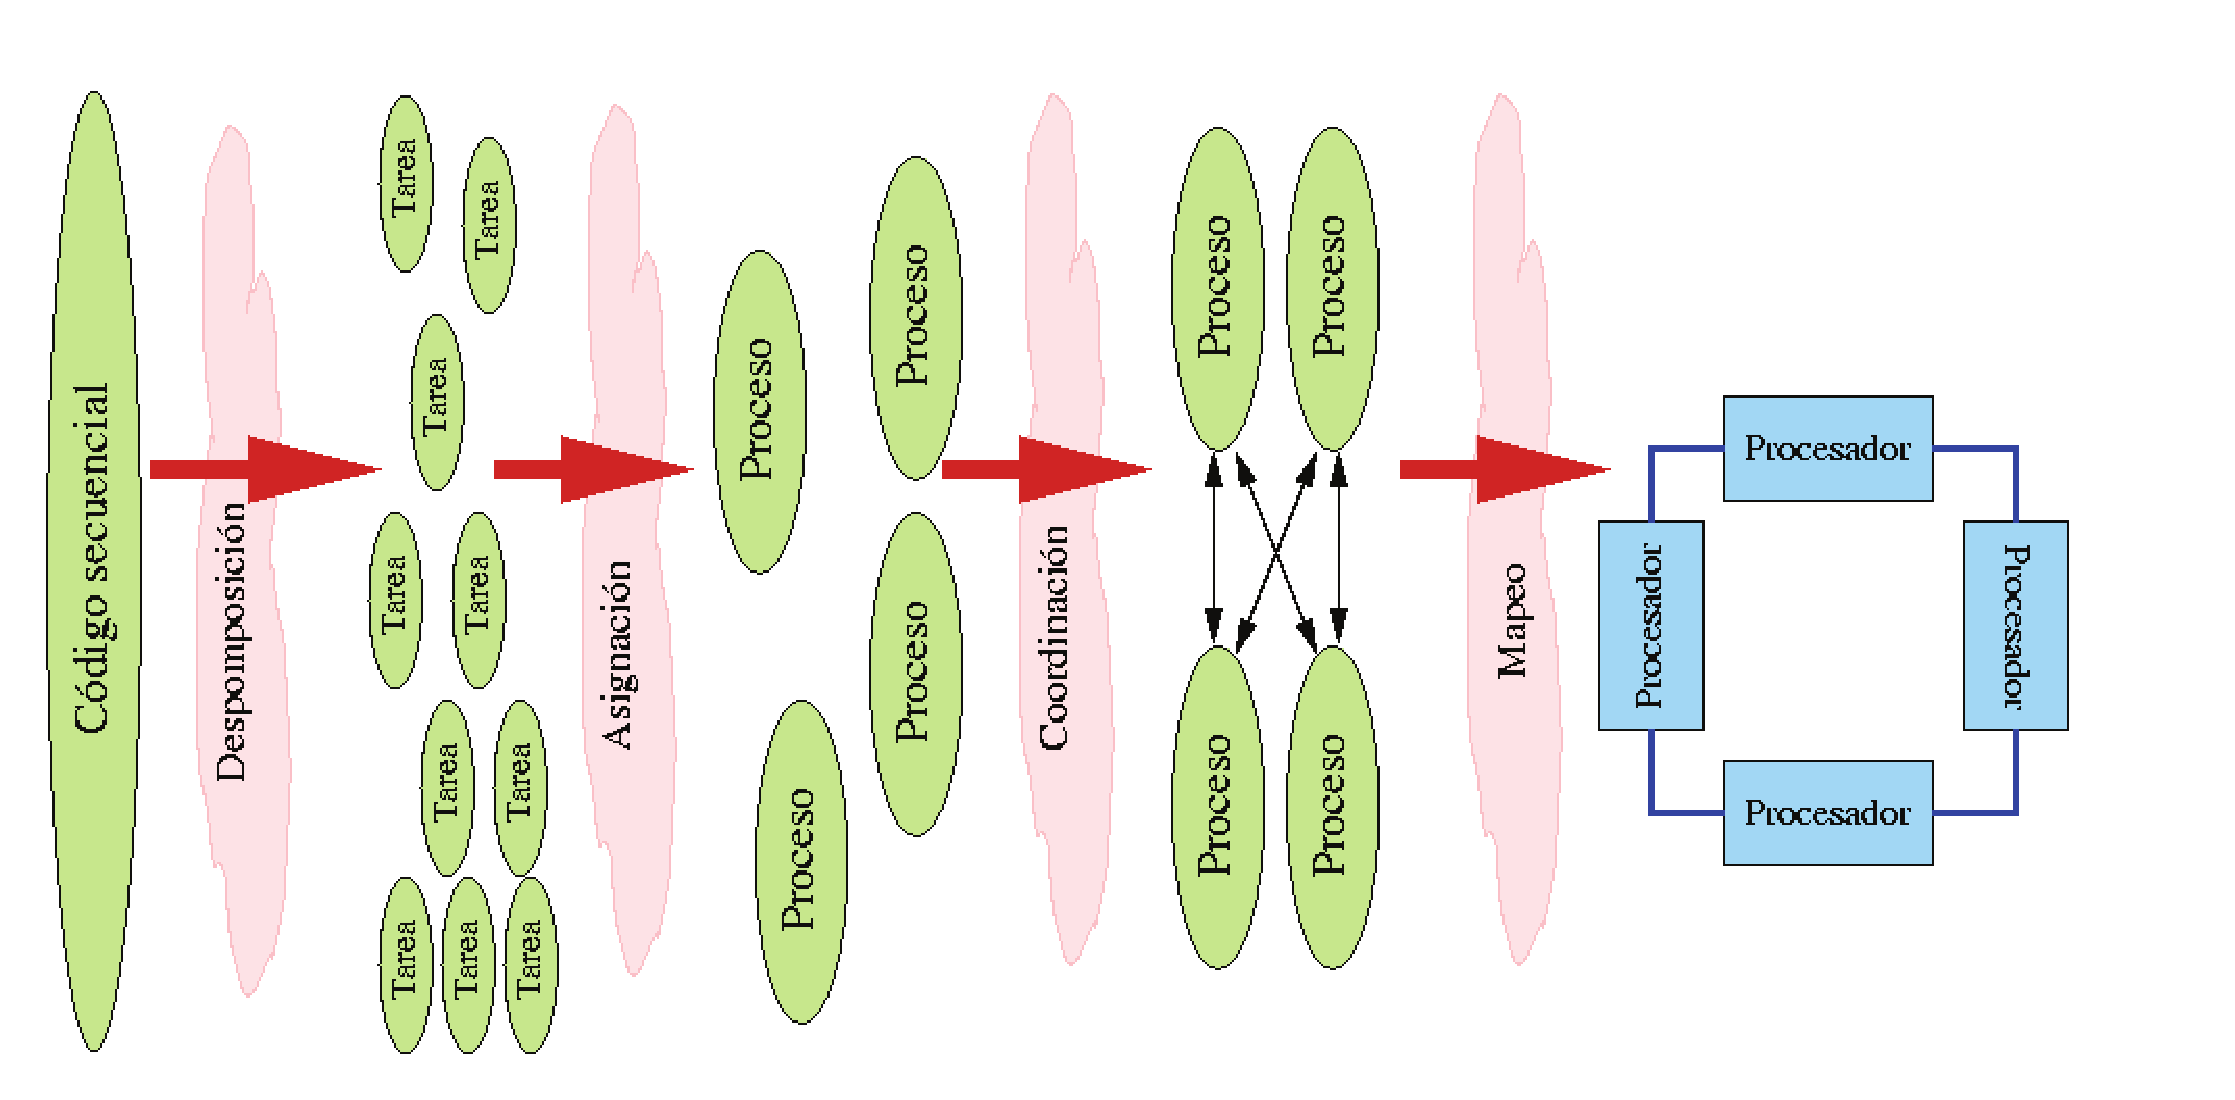
\includegraphics[width=15cm]{figuras/figura01.eps}}
\caption{Esta é a figura de tal e cal.}
\label{enlace1}
\end{figure}

\begin{table}
\begin{center}
\begin{tabular}{|l||r|c|} \hline
Izquierda & Derecha & Centrado  \\ \hline\hline
ll & r & cccc \\ \hline
llll & rrr & c \\ \hline
\end{tabular}
\caption{Esta é a táboa de tal e cal.}
\label{enlace2}
\end{center}
\end{table}

\section{Exemplos de referencias á bibliografía}
Este é un exemplo de referencia a un documento descargado da web \cite{cuda}. E este é un exemplo de referencia a unha páxina da wikipedia \cite{cdma}. Agora un libro \cite{gonzalez} e agora unha referencia a un artigo dunha revista \cite{patricia}. Tamén se poden pór varias referencias á vez \cite{cuda,gonzalez}.

\section{Exemplos de enumeracións}

Con puntos:

\begin{itemize}
\item Un.
\item Dous.
\item Tres.
\end{itemize}

Con números:

\begin{enumerate}
\item Catro.
\item Cinco.
\item Seis.
\end{enumerate}

Exemplo de texto verbatim:

\begin{verbatim}
O texto        verbatim 
     se visualiza tal
            como se escribe
\end{verbatim}

Exemplo de código C:

\lstset{language=C}

\begin{lstlisting}
#include <math.h>
main()
{  int i, j, a[10];
   for(i=0;i<=10;i++) a[i]=i; // comentario 1
   if(a[1]==0) j=1; /* comentario 2 */
   else j=2;
}
\end{lstlisting}

Exemplo de código Java:

\lstset{language=java}

\begin{lstlisting}
class HelloWorldApp {
    public static void main(String[] args) {
        System.out.println("Hello World!"); // Display the string.
    }
}
\end{lstlisting}



\cleardoublepage
% Fin de la sección de ejemplos


\chapter{Conclusiones y posibles ampliaciones}

\todo{ Completar conclusiones y posibles ampliaciones}

%----------Ampliaciones----------%
 
%	- Discretización de estados con redes neuronales (mirar correo de pablo pra o nombre).
%	- Q Learning completo.
%	- Aumento de las posibles acciones y estados con más mecánicas.
%	- Realización de numerosas pruebas contra jugadores humanos.
%	- Implementación para otros sistemas operativos.

%----------------------------------%

% Aquí empiezan los apéndices
\appendix
\cleardoublepage
\chapter{Manual técnico}


Este manual técnico está dedicado a que cualquier tipo de usuario pueda poner en funcionamiento la aplicación desarrollada en este trabajo, tanto el videojuego en si mismo como el agente que contiene. 

\section{Requisitos de instalación}

En términos de requisitos necesarios del sistema solo existe uno referente al sistema operativo. Se garantiza el funcionamiento de la aplicación en versiones de \textbf{macOS superiores a 10.12}. Para probar esto se han utilizado varios equipos con esta versión del sistema distintos del equipo de desarrollo.

\bigskip

Además es deseable contar con un chip de gráficos, ya sea integrado en el procesador o externo dado que para cualquier videojuego con requisitos de rendimiento se benefician mucho de los mismos. En concreto esta aplicación no necesita demasiados recursos en este sentido pues la escena principal de \textit{gameplay} se dibuja internamente a una resolución muy reducida de 400x300.

\section{Instrucciones de instalación}

Dado que la aplicación es auto-contenida\footnote{La aplicación no solo contiene el programa compilado sino todos los frameworks, librerías dinámicas, imágenes, sonidos y otros archivos necesarios para su funcionamiento en su interior} simplemente se tiene que contar con el archivo ejecutable \textit{\textbf{It\_Fights.app}}. No existen pasos requeridos para su instalación concretos, simplemente se requiere, como es lógico, que el usuario que vaya a ejecutar la aplicación tenga permisos de lectura y ejecución sobre dicho ejecutable.

\section{Ejecución de la aplicación}
\label{sec:ejecucion}
La aplicación puede ser muy fácilmente ejecutada desde el sistema de archivos de macOS, simplemente se deberá hacer clic en el archivo \textbf{\textit{It\_Fights.app}} y se abrirá la ventana con la aplicación.

\bigskip

Si se desea tener acceso al ejecutable interno o ejecutarlo desde la consola del sistema para ver la salida de los combates simulados en ella se podrá hacer siguiendo los siguientes pasos:

\begin{enumerate}
	\item Abrir la terminal.
	\item Ir a la ruta en la que se encuentre la aplicación \textbf{\textit{It\_Fights.app}}.
	\item Entrar en ella como si fuera un directorio con:
		\begin{lstlisting}
	cd It_Fights.app/Contents/
		\end{lstlisting}
	\item Se puede ver la estructura interna que contiene los frameworks, información del ejecutable, librerías y otros archivos con:
		\begin{lstlisting}
	ls
		\end{lstlisting}
	\item El ejecutable interno estará en la carpeta \textbf{\textit{MacOS}} a la que se entra con:
		\begin{lstlisting}
	cd MacOS
		\end{lstlisting}
	\item Finalmente podremos ejecutar el programa con el comando:
		\begin{lstlisting}
	./It_Fights  
		\end{lstlisting}
\end{enumerate}


\cleardoublepage
\chapter{Manual de usuario}

Pese a que se ha priorizado la usabilidad de la aplicación durante su desarrollo, en este apartado se especificarán los pasos a seguir para utilizar las funcionalidades que ofrece, ayudándonos de capturas cuando sea necesario. La parte más importante de este manual de usuario es la sección dedicada a mostrar los botones del mando que se pueden usar en cada escena del juego y las funcionalidades que ofrecen.

\section{Instalación/Ejecución de la aplicación}

Pese a que se trate este aspecto de una forma completa en el apartado \ref{sec:ejecucion} del manual técnico, a nivel de usuario la forma ideal de comenzar la ejecución del programa es simplemente utilizar la interfaz del sistema de archivos de macOS y hacer doble \textit{click} sobre el ejecutable llamado \textbf{\textit{It\_Fights.app}}. No hay pasos relacionados con la instalación en si misma sino que simplemente se debe de estar en posesión del ejecutable.


\section{Controles de la aplicación}
\label{sec:controles}
Desde el punto de vista de un usuario común, la aplicación prioriza el uso único del mando. Para explicar el funcionamiento de cada uno de los botones (o los equivalentes en mandos de otras marcas) se hará uso de la figura \ref{controles:mando}\footnote{imagen oficial de la documentación de Microsoft extraída de: \\ \url{https://support.xbox.com/es\-ES/xbox\-360/accessories/controllers}}.

\begin{figure}
	\centerline{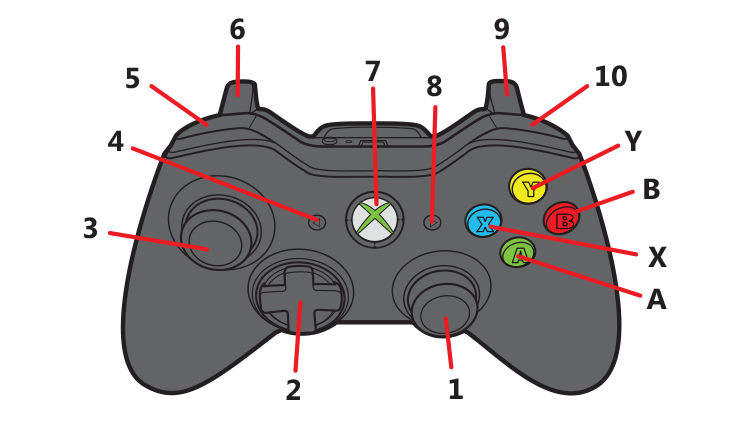
\includegraphics[width=12cm]{otros/graphicalInterface/mando.png}}
	\caption{Mando de Xbox360}
	\label{controles:mando}
\end{figure}

\subsection{Controles del menú}

Los controles de la escena del menú a la hora de usar el mando son los siguientes:

\begin{itemize}
	\item \textbf{\textit{D-Pad}}: Identificado con el número \textbf{2} en la figura \ref{controles:mando}. Usado para mover arriba y abajo las opciones seleccionadas del menú, mover el D-PAD a izquierda y derecha no tendrá efecto.
	\item \textbf{\textit{Botón X}} Identificado con la letra \textbf{X} en la figura \ref{controles:mando}. Usado para ejecutar la opción seleccionada actualmente.
\end{itemize}

\subsection{Controles de combate}

Los controles a la hora de controlar a uno de los jugadores (o a ambos si se dispone de dos mandos conectados en la opción de jugador contra jugador) son los siguiente:

\begin{itemize}
	\item \textbf{\textit{Joystick izquierdo}}: Identificado con el número \textbf{3} en la figura \ref{controles:mando}. Usado para mover al jugador en cualquier dirección (360 grados). Si se inclina ligeramente el movimiento del personaje será más lento permitiendo variar la velocidad del mismo.
	\item \textbf{\textit{Botón A}} Identificado con la letra \textbf{A} en la figura \ref{controles:mando}. Usado para realizar un ataque en la dirección en la que se está mirando.
	\item \textbf{\textit{Botón B}} Identificado con la letra \textbf{B} en la figura \ref{controles:mando}. Usado para realizar una acción defensiva o \textit{parry}\footnote{término usado en esgrima para bloquear y/o reflejar un ataque inminente hacia el contrincante} en la dirección que se está mirando.
	\item \textbf{\textit{Botón Back}} Identificado con el número \textbf{4} en la figura \ref{controles:mando}. Usado para volver al menú saliendo de la pelea.
\end{itemize}

\subsection{Controles avanzados}

Además, se pueden usar las flechas del teclado para iterar sobre las opciones del menú y la tecla \textit{intro} para ejecutar la opción. Otra opción disponible es abrir y cerrar la consola de la aplicación al introducir el carácter del teclado \textbf{\textbackslash} conocido como \textbf{barra invertida}. Con la consola abierta, todos los caracteres que introduzcamos con el teclado se agregarán a la línea de entrada de la consola. Además podremos usar la tecla \textit{intro} para confirmar el comando introducido. \textbf{Importante}: Esta opción está disponible solamente para usuarios avanzados y preferentemente con conocimiento interno de la aplicación por lo que no se incluirán una lista de los mensajes permitidos.

\section{Uso de las diferentes escenas}

Utilizaremos esta sección para mostrar una vista de las escenas que se pueden dar y especificar el comportamiento de las mismas de cara al usuario o jugador.

\bigskip

Como nota adicional se mencionará aquí la posibilidad de cambiar el tamaño de la ventana de la aplicación en cualquier momento. Al hacerlo siempre se mantendrá la relación de aspecto y se escalará la imagen vista para que no se produzcan errores visuales.

\subsection{Uso del menú}

\begin{figure}[h]
	\centerline{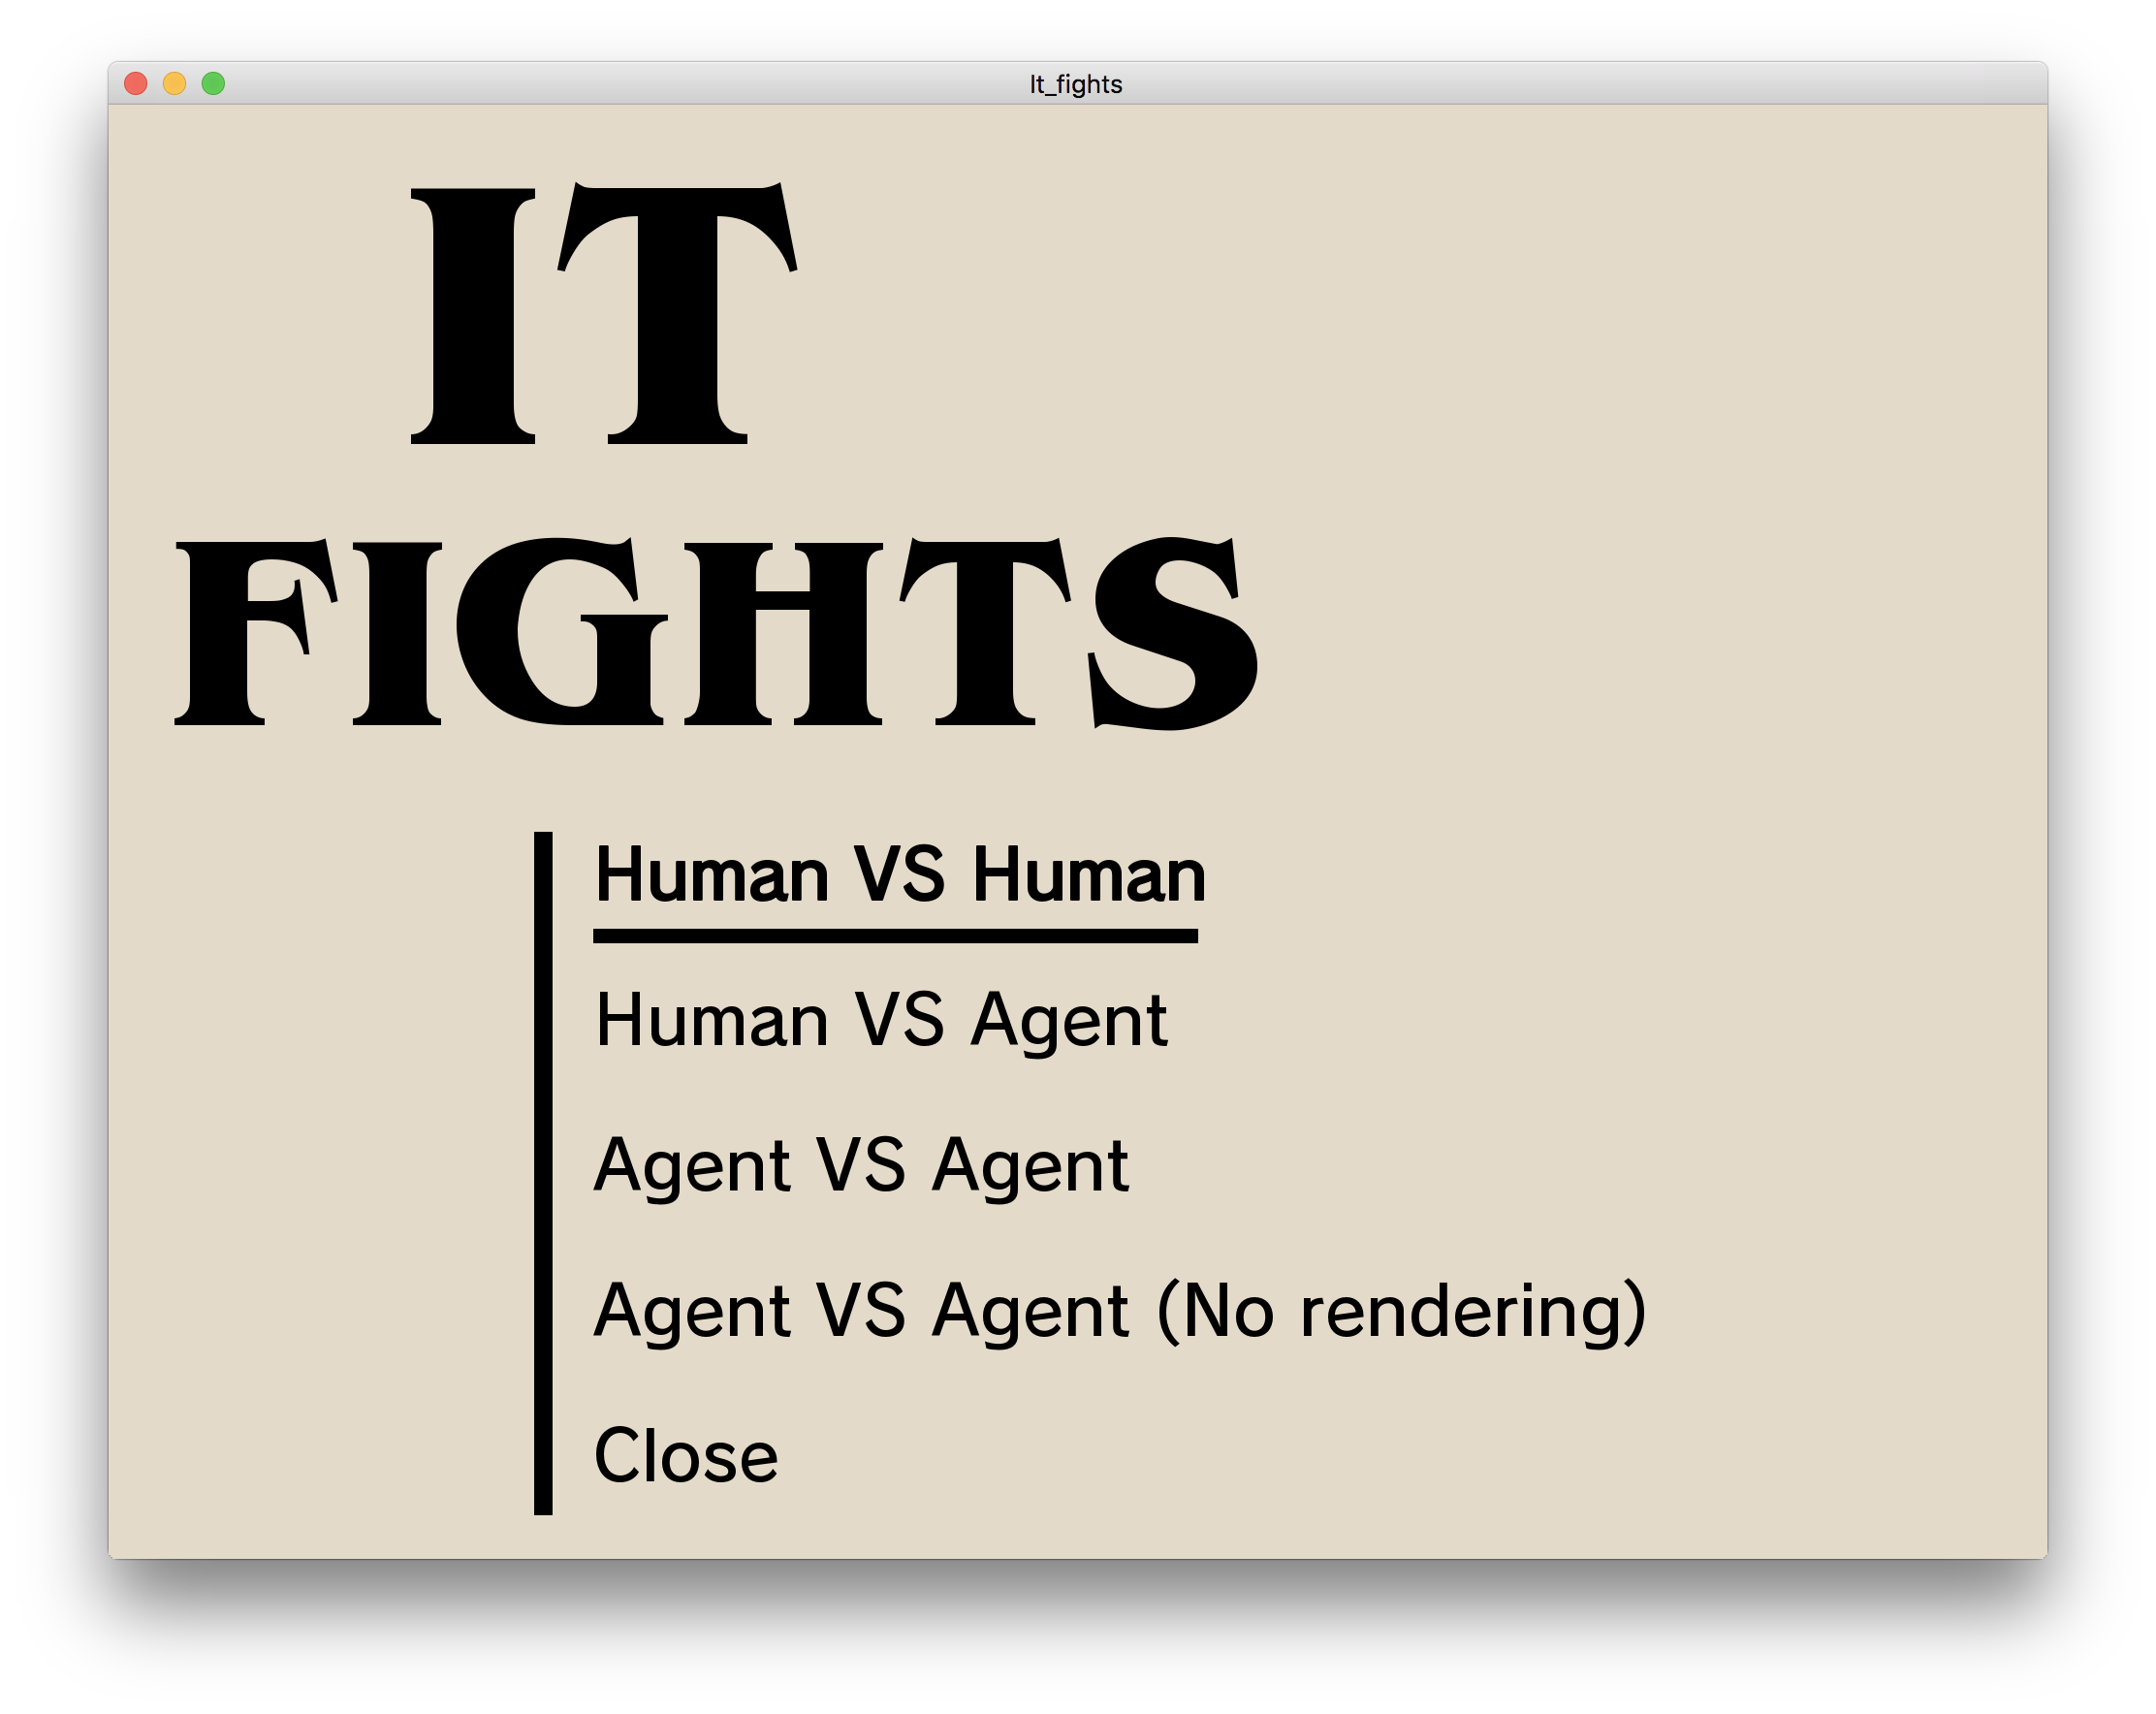
\includegraphics[width=17cm]{otros/manual/menu1.png}}
	\caption{Menú al iniciar la aplicación}
	\label{uso:menu}
\end{figure}

\begin{figure}[h]
	\centerline{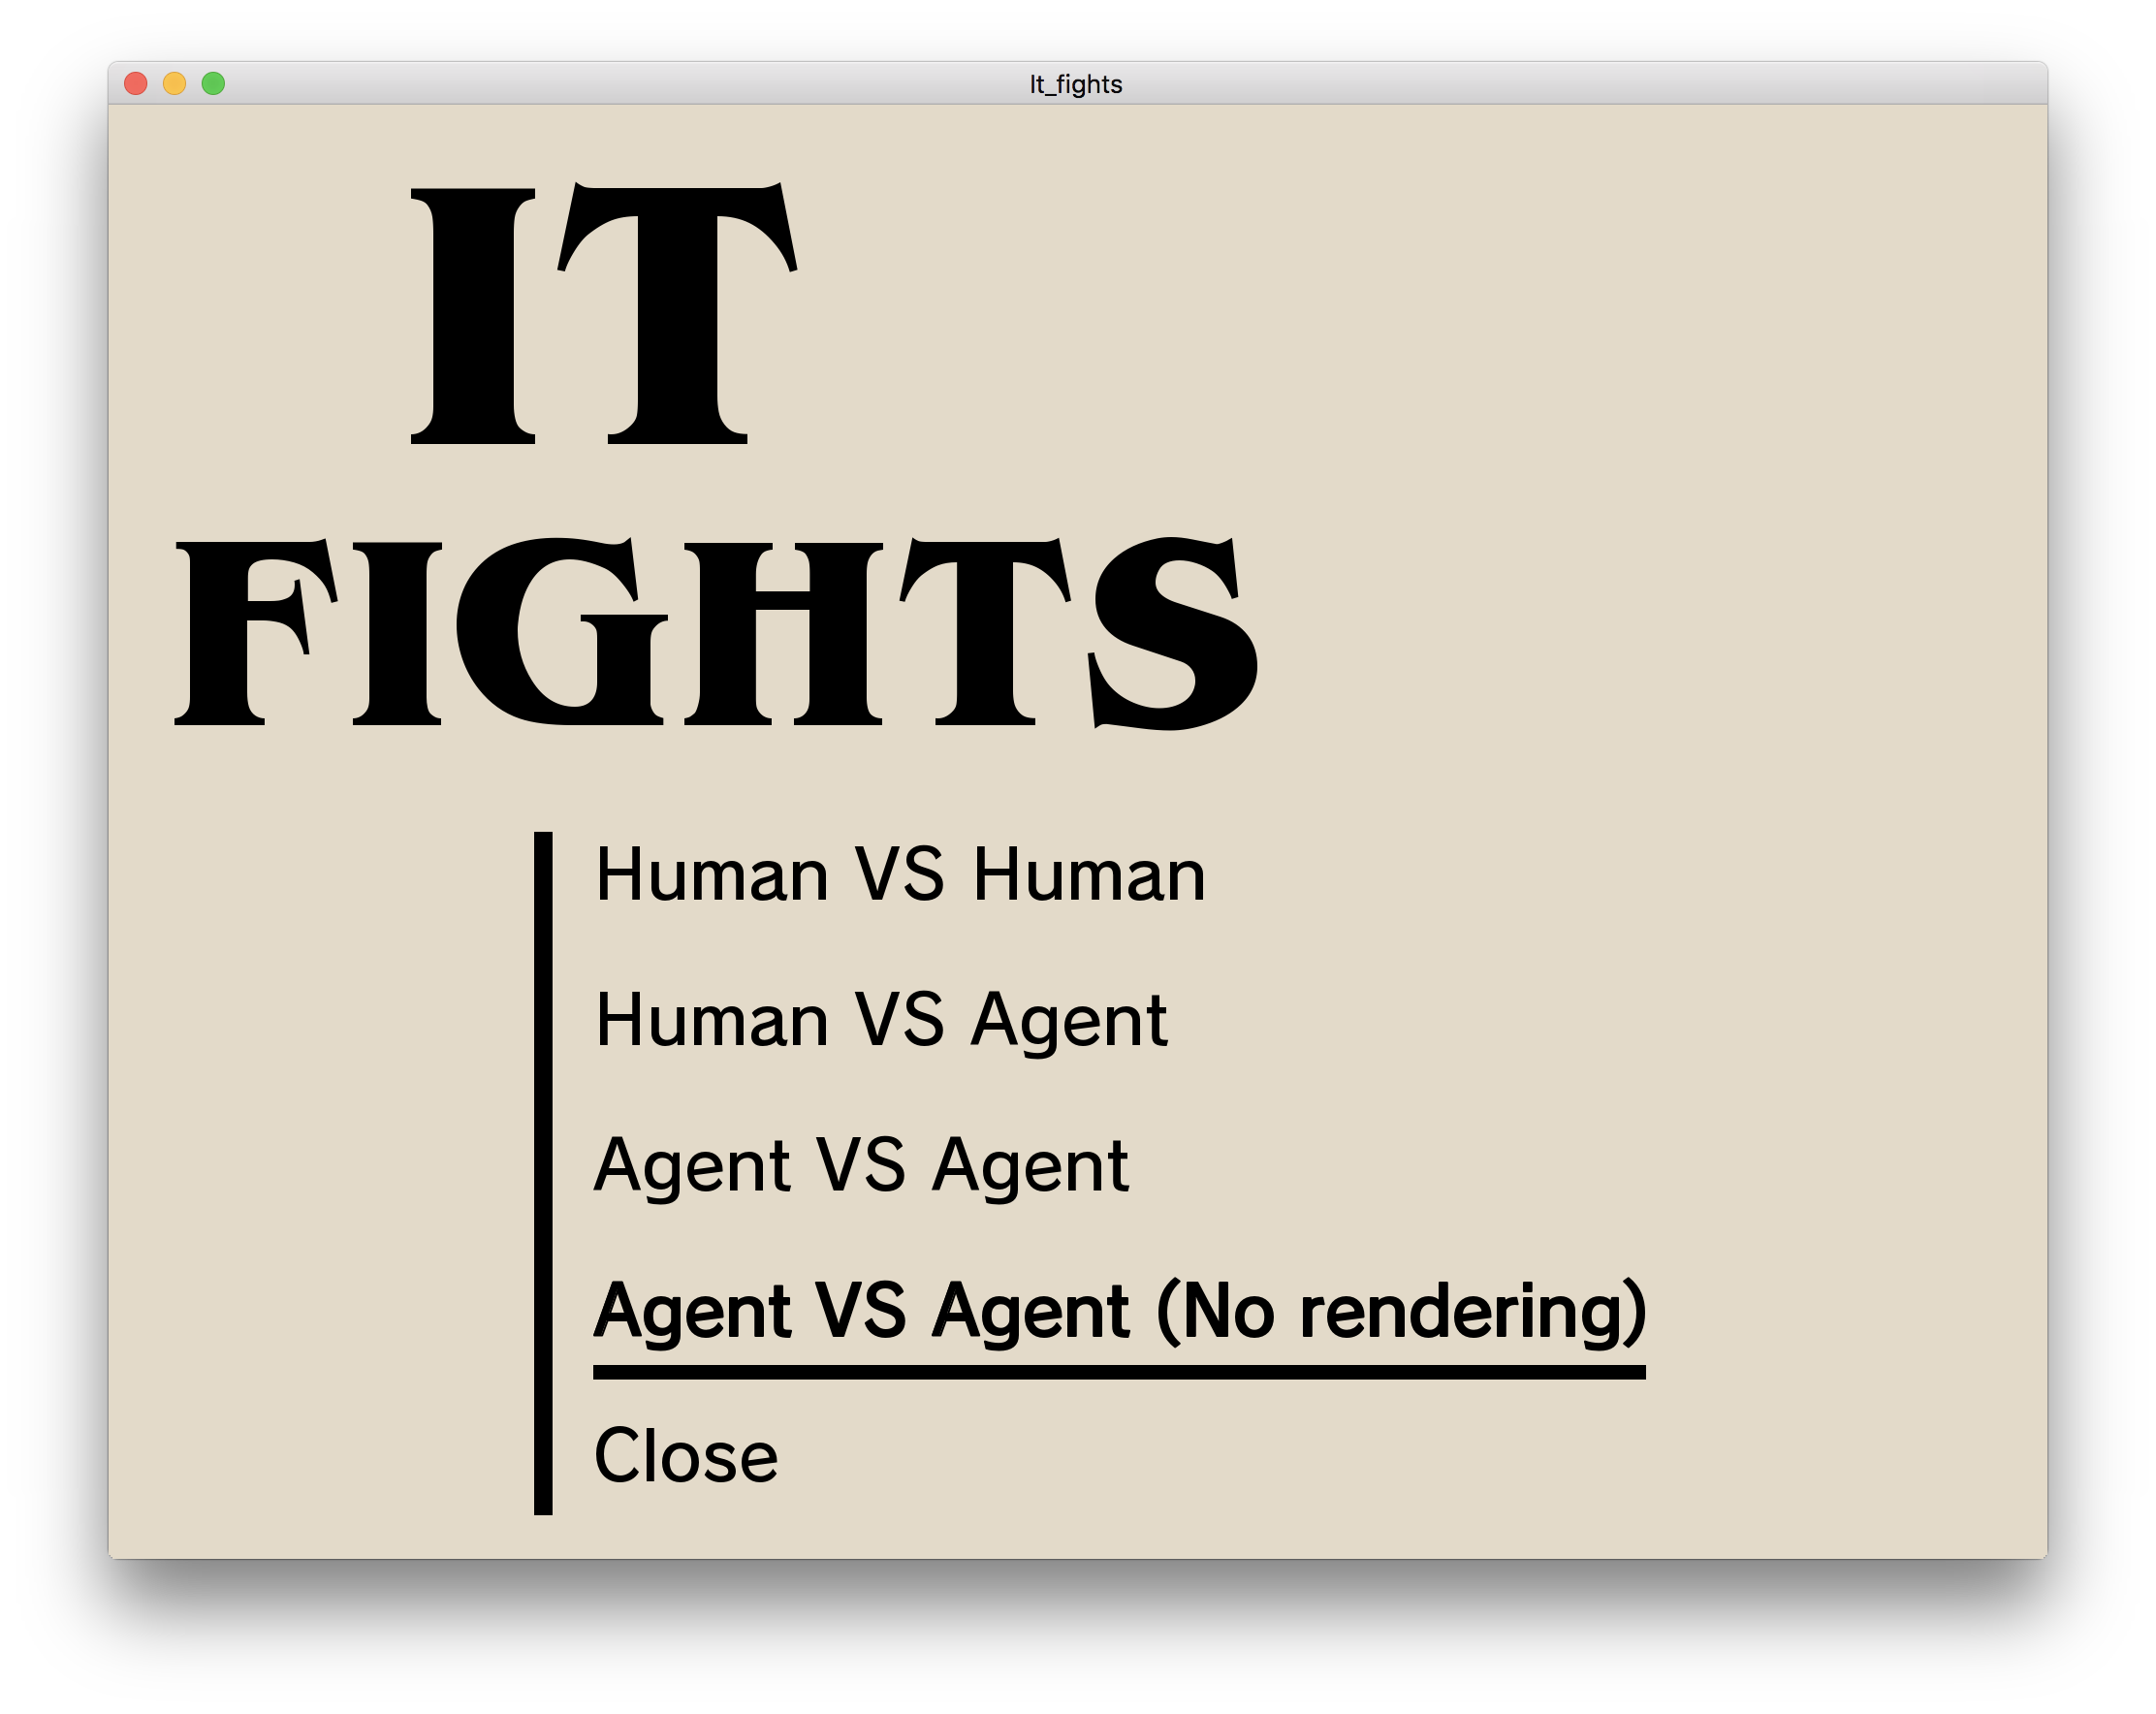
\includegraphics[width=17cm]{otros/manual/menu2.png}}
	\caption{Menú al cambiar de opción}
	\label{uso:menu2}
\end{figure}

En las figuras \ref{uso:menu} y \ref{uso:menu2} vemos el menú de la aplicación. En la primera figura (\ref{uso:menu}) se observa como la opción preseleccionada por defecto es la primera, si movemos con el D-PAD o el las flechas del teclado la selección o bien dos veces arriba o tres veces abajo llegaremos a la opción mostrada en la segunda figura (\ref{uso:menu}). Al cambiar de opción se moverá la barra que subraya la nueva opción seleccionada, dicha opción también se mostrará en negrita y se oirá un sonido similar a un silbido al realizar dicho cambio.

\bigskip

Al pulsar el botón de ejecutar (\textbf{X}) se ejecutará la opción seleccionada en ese momento, la ejecución de cada opción implica las siguientes acciones:

\begin{enumerate}
	\item \textbf{\textit{Human VS Human}}: Se comienza el combate entre dos jugadores (necesarios dos mandos conectados al equipo para controlar a ambos).
	\item \textbf{\textit{Human VS Agent}}: Se comienza el combate contra el agente que ha aprendido previamente.
	\item \textbf{\textit{Agent VS Agent}}: Se enfrentan dos enemigos, el basado en reglas y el agente que ha aprendido.
	\item \textbf{\textit{Agent VS Agent (No Rendering)}}: Se enfrentan los dos enemigos durante 100 simulaciones, las mismas no se mostrarán por pantalla (\textbf{Importante}: Solo con fines de demostración, para mostrar las capacidades y rendimiento del motor y del agente).
	\item \textbf{\textit{Close}}: Cierra la ventana y la aplicación.
\end{enumerate}

\subsection{Combate}

\begin{figure}[h]
	\centerline{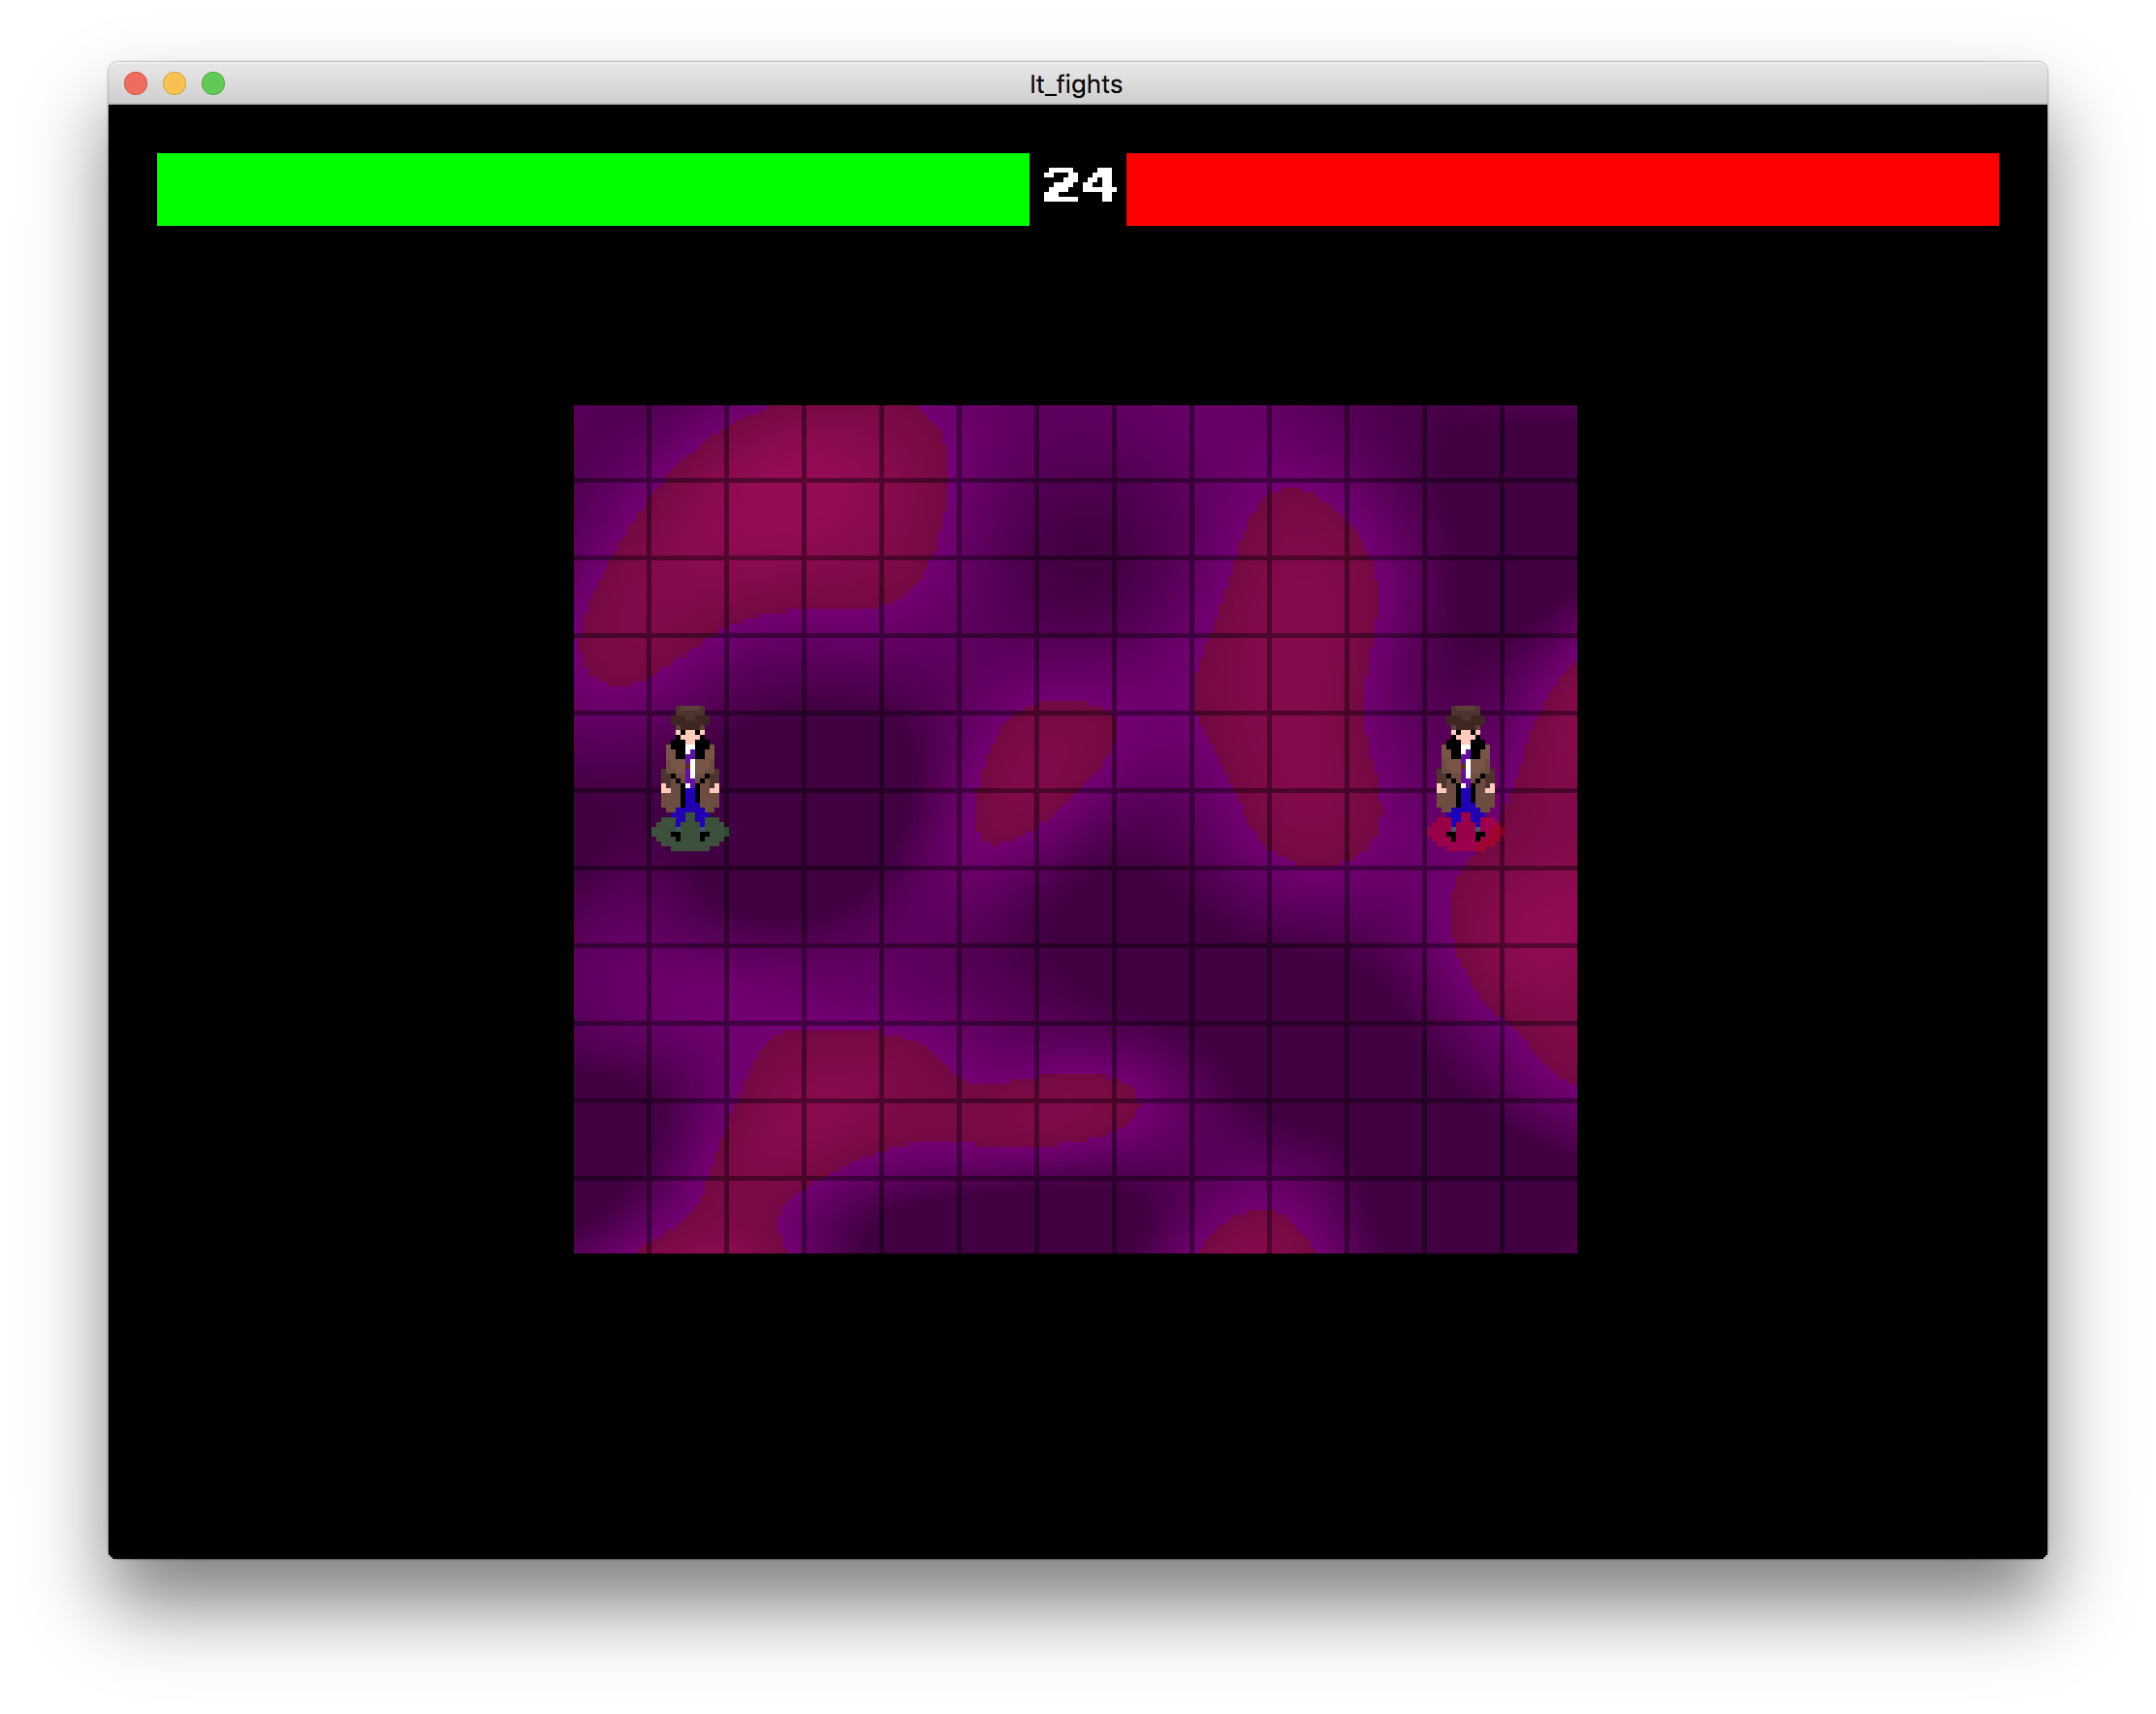
\includegraphics[width=17cm]{otros/manual/pelea1.png}}
	\caption{Inicio del combate}
	\label{uso:pelea1}
\end{figure}


\begin{figure}[h]
	\centerline{
\includegraphics[width=14cm]{otros/manual/atacando1.png}}
	\caption{Personaje atacando}
	\label{uso:ataque}
\end{figure}

\begin{figure}[h]
	\centerline{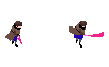
\includegraphics[width=14cm]{otros/manual/parry.png}}
	\caption{Personaje haciendo \textit{parry}}
	\label{uso:parry}
\end{figure}


Si se elige una de las dos primeras opciones se entrará en una escena de combate en la que se puede controlar al jugador, dicha escena se puede ver en la figura \ref{uso:pelea1}. Las mecánicas del combate son las siguientes:

\begin{itemize}
	\item \textbf{Moverse}: El personaje se moverá en la dirección deseada. Se puede reducir la velocidad de movimiento reduciendo el ángulo del \textit{joystick}. El personaje estará mirando siempre para la dirección en la que se está moviendo o la última en la que se ha movido si está quieto.
	\item \textbf{Atacar}: Al atacar el personaje realizará una animación en la dirección en la que se está mirando, si el enemigo está en esa dirección y a rango de ataque será dañado a menos que esté realizando un \textit{parry}. El ataque implica un pequeño desplazamiento del personaje hacia delante. Se puede ver en la figura \ref{uso:ataque}.
	\item \textbf{Defenderse o \textit{parry}}: Al realizar un \textit{parry} el personaje será invulnerable durante medio segundo. Sin embargo, si durante ese medio segundo no se para ningún ataque se entrará en un periodo de descanso durante otro medio segundo donde no se podrá mover, atacar o defenderse. Si por el contrario sí se defiende con éxito entonces se podrá realizar un ataque gratuito al personaje enemigo. Se puede ver en la figura \ref{uso:parry}.
	\item \textbf{Salir de la partida}: Se sale del combate volviendo al menú de la aplicación. 
\end{itemize}


\subsection{Consola}

\begin{figure}[h]
	\centerline{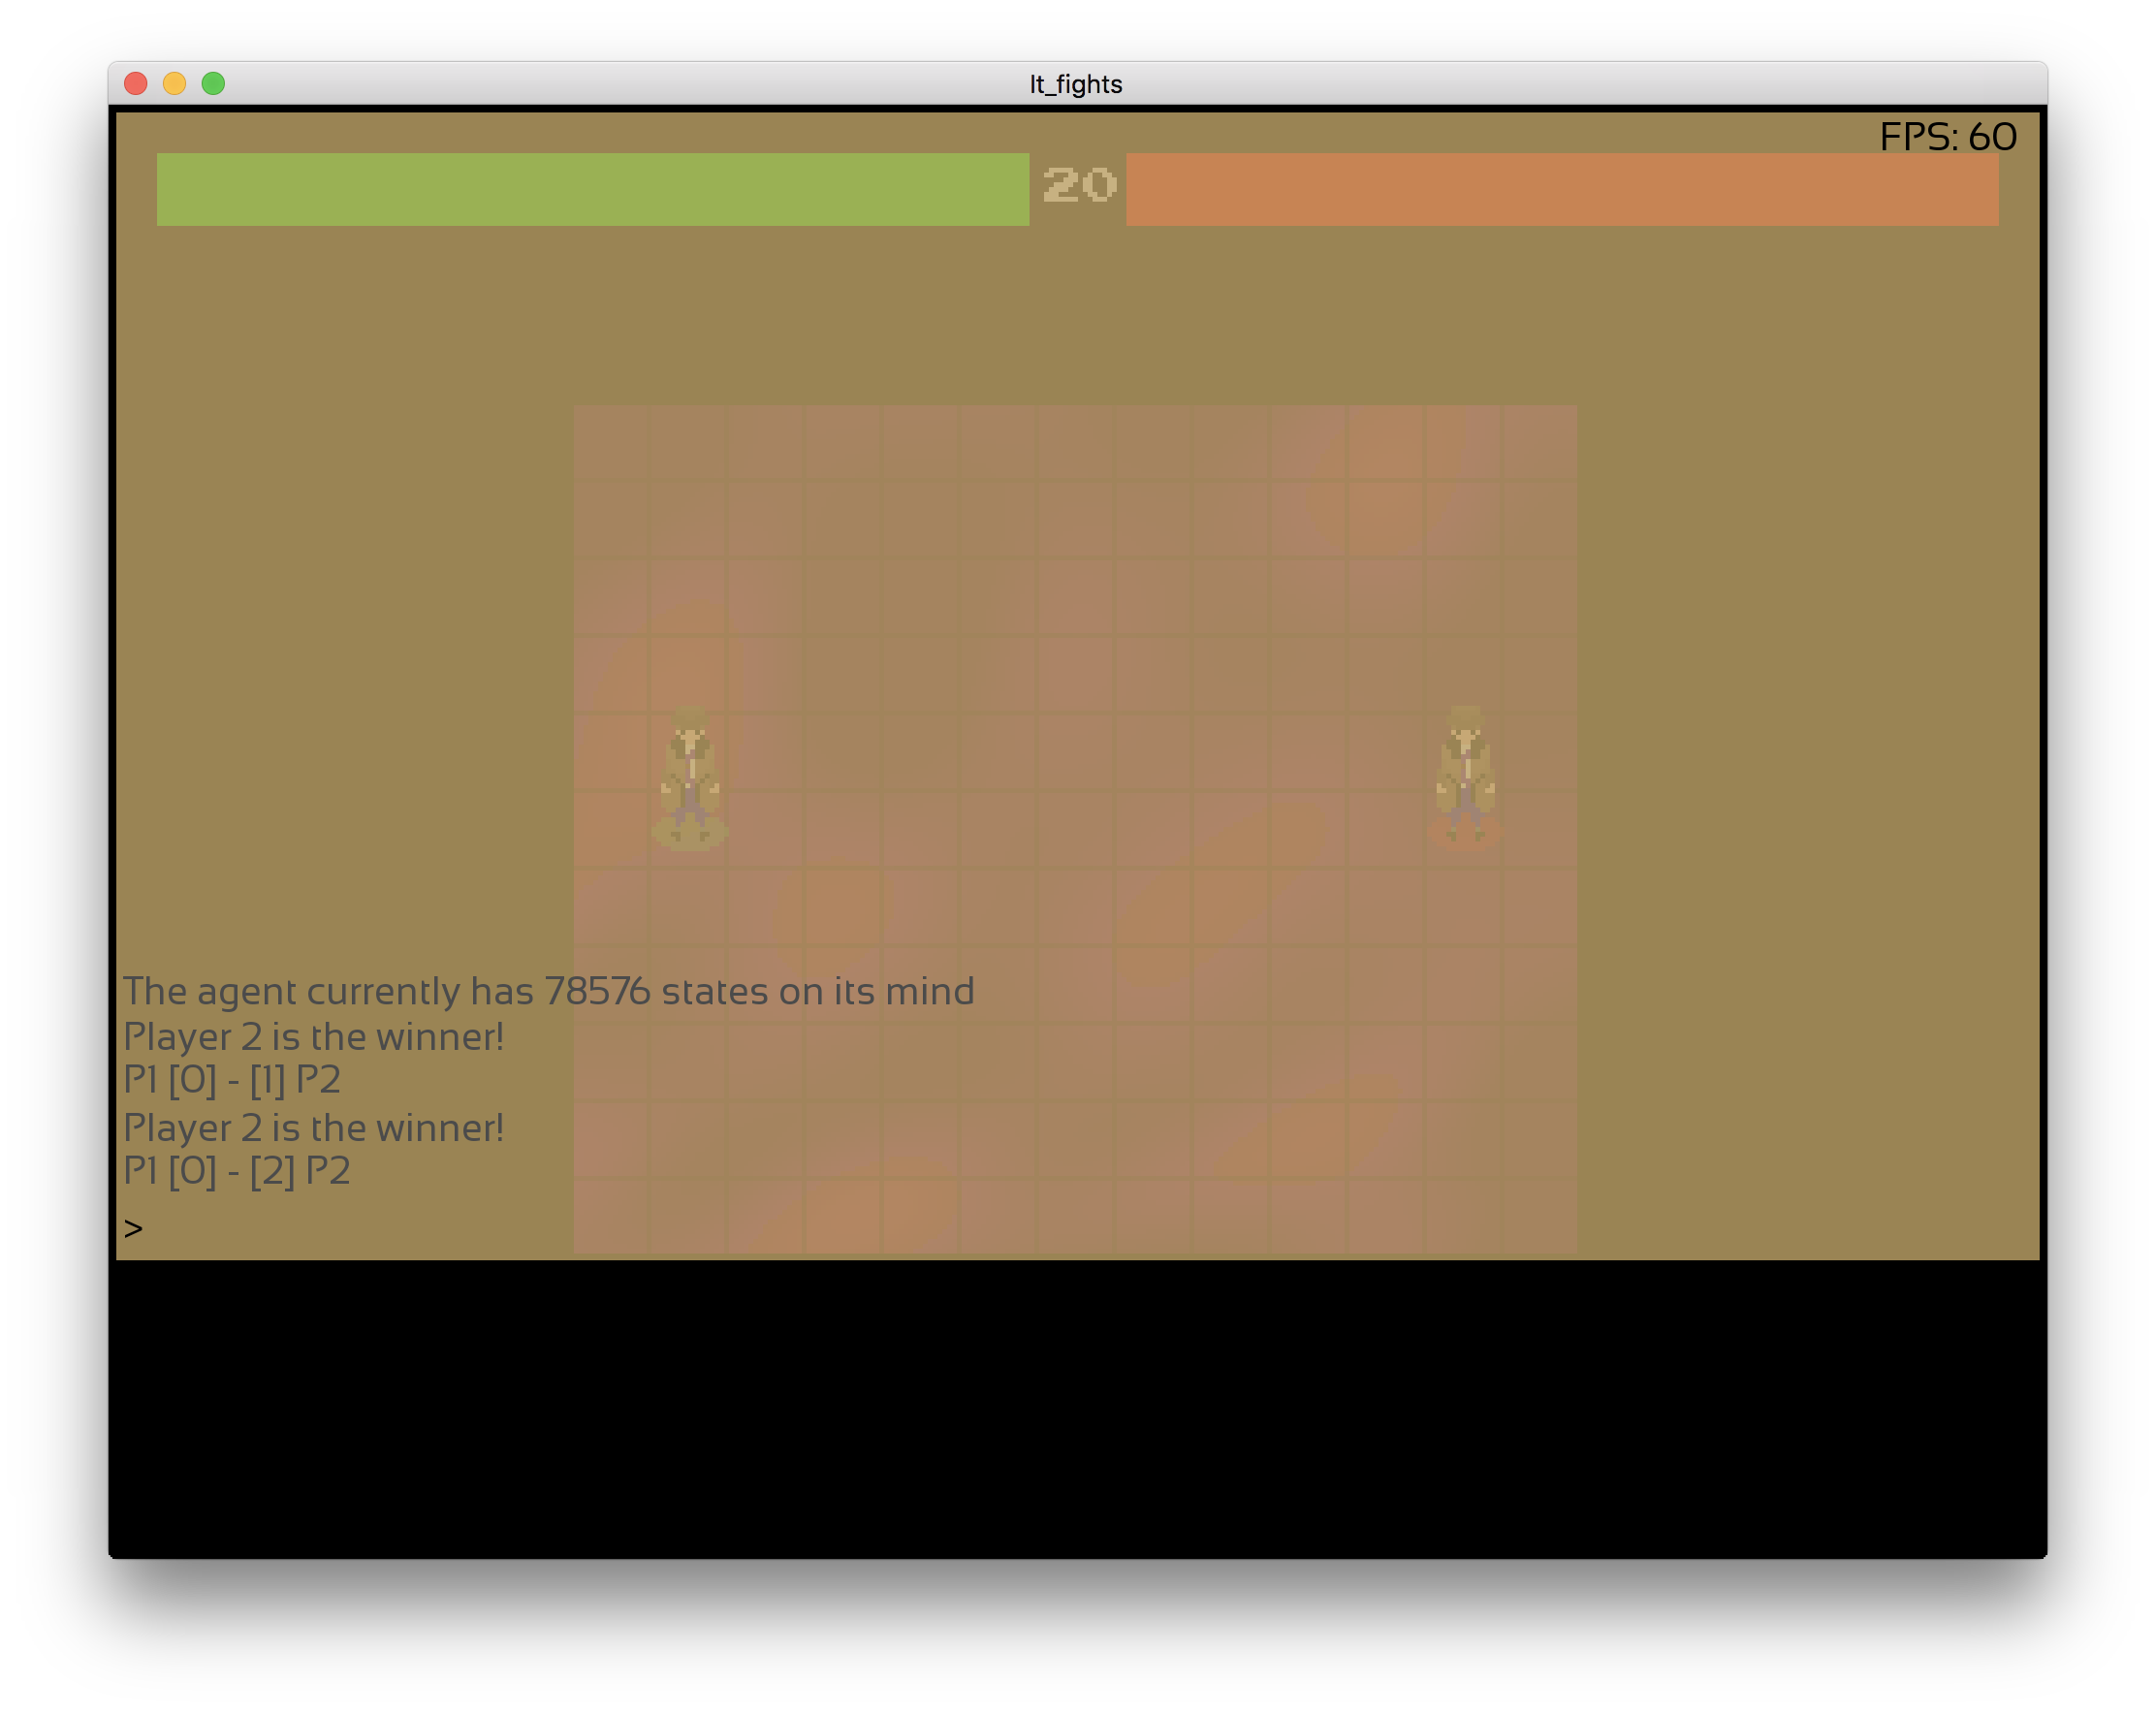
\includegraphics[width=17cm]{otros/manual/consola.png}}
	\caption{Consola abierta en la escena de combate}
	\label{uso:consola}
\end{figure}

Por último, se puede observar la consola abierta durante la escena de combate en la figura \ref{uso:consola}, la misma se puede abrir en cualquier momento del juego excepto cuando se están realizando las simulaciones sin \textit{renderizado} ya que no se muestra nada por pantalla para acelerar el proceso.

\bigskip

Con la consola abierta podemos ver los diferentes mensajes que se muestran en ella, en el caso de esta figura (\ref{uso:consola}) se puede ver el número de estados que había visitado el agente y las veces que uno de los personajes ha ganado al otro en esta ejecución.

\bigskip

Finalmente, se muestran los fotogramas por segundo o \textbf{\textit{FPS}} en la esquina superior derecha para ayudar a reconocer problemas de rendimiento si fuera necesario.



\cleardoublepage
\chapter{Licencia}

\todo{Insertar licencia apropiada}

\cleardoublepage
\markboth{BIBLIOGRAFÍA}{BIBLIOGRAFÍA}
\addcontentsline{toc}{chapter}{Bibliografía}

\todo {Completar bibliografía}

\begin{thebibliography}{99}
	
\bibitem{definiendo_arquitectura} Definición de arquitectura según la ISO/IEC/IEEE 42010:2011. Artículo referenciado ({\it http://www.iso-architecture.org/ieee-1471/defining-architecture.html}). Consultado el 2 de junio de 2017.

\bibitem{modelado_referencia}Grady Booch, James Rumbaugh, and Ivar Jacobson. El lenguaje unificado de modelado. Manual
de referencia. Addison Wesley, 1999.

\bibitem{ieee}IEEE recommended practice for software requirements specifications. Technical report, 1998.
	
% ----------------EJEMPLOS--------------------	
% EXEMPLO DE DOCUMENTO DESCARGADO DA WEB
\bibitem{cuda} Nvidia CUDA programming guide. Versión 2.0, 2010. Dispoñible en {\it http://www.nvidia.com}.

% EXEMPLO DE PÁXINA DA WIKIPEDIA
\bibitem{cdma} Acceso múltiple por división de código. Artigo da wikipedia ({\it http://es.wikipedia.org}). Consultado o 2 de xaneiro do 2010.

% EXEMEPLO DE LIBRO
\bibitem{gonzalez} R.C. Gonzalez e R.E. Woods, {\it Digital image processing}, 3ª edición, Prentice Hall, New York, 2007.

% EXEMPLO DE ARTIGO DE REVISTA
\bibitem{patricia} P. González, J.C. Cartex e T.F. Pelas, ``Parallel computation of wavelet transforms using the lifting scheme'', {\it Journal of Supercomputing}, vol. 18, no. 4, pp. 141-152, junio 2001.
\end{thebibliography}





% Aquí mostramos la lista de TODOs que tendremos que quitar al terminar el documento
\cleardoublepage
\todo{Quitar la lista de TODOs}
\listoftodos
\cleardoublepage
% Fin de la lista de TODOs

\end{document}
